\documentclass[11pt,a4paper,oneside]{report}

%%% Title of this document, updated automatically in the title page and references
\title{Design review and recommendations}

\makeatletter
\let\documenttitle\@title
\makeatother

%%% PACKAGES
\usepackage[	bookmarks,%
		breaklinks,%
		backref=false,%
		pdfhighlight=/I,%
		pdffitwindow=true,%
		pdfstartview=Fit,%
		pdfcenterwindow=true,%
		%linkbordercolor={0.4 0.4 1},% change border colour
		colorlinks = false, % switch off colour linked text
		pdfborder={0 0 0}, % switch off colour linked text
		pdftitle=\documenttitle,%
		pdfauthor=Artur K. Lidtke and Aleksander A. Lidtke]%
		{hyperref} % cross-refenreces

\usepackage{amsmath} % general maths
\usepackage[square,sort,comma,numbers]{natbib} % bibliography; options needed to make it work with Mendeley & sorted citations
\usepackage{booktabs} % ?
\usepackage{graphicx} % figures
\usepackage{times} % font for main text \textrm
\usepackage{helvet} % font for sans serif bits \textsf
\usepackage{sectsty} % separate format for section headings
\usepackage[varg]{txfonts} % ?
\usepackage{todonotes} % notes
\usepackage{verbatim} % ?
\usepackage{changepage} % local changes to margins, etc.
\usepackage{setspace} % setstretch for linespacing
%\usepackage{indentfirst} % indent the 1st paragraph of each section just as any other one
\usepackage[nottoc]{tocbibind} % add table of figures, tables and bibliography in the contents

\usepackage{color}
\usepackage{listings}
\definecolor{codegreen}{rgb}{0,0.6,0}
\definecolor{codegray}{rgb}{0.5,0.5,0.5}
\definecolor{codepurple}{rgb}{0.58,0,0.82}
\definecolor{blue}{rgb}{0.1,0.1,1.0}
 
\lstdefinestyle{myPythonStyle}{
    commentstyle=\color{codegreen},
    keywordstyle=\color{magenta},
    numberstyle=\tiny\color{codegray},
    stringstyle=\color{codepurple},
    basicstyle=\footnotesize,
    breakatwhitespace=false,         
    breaklines=true,                 
    captionpos=b,                    
    keepspaces=true,                 
    showspaces=false,                
    showstringspaces=false,
    showtabs=false,                  
    tabsize=2
}
 
\setcounter{tocdepth}{2} % exclude subsubsections from the ToC

\usepackage{hhline} % double line in tables
\usepackage{array} % table formatting
\usepackage{float} % for figures in tabular form
\usepackage{subfig} % --||--
\usepackage{xspace} % smartly add or not a space at the end of macro expressions

\usepackage{fancyhdr} % header/footer
\usepackage{emptypage} % empty cleardoublepage
\usepackage{etoolbox} % change page format using patchcmd

\usepackage{titlesec} % detailed formatting of specific headings
\usepackage{pdfpages}

\usepackage{units}

\graphicspath{{Figures/}} % where all the Figures are held

\allsectionsfont{\sffamily} % set sections font to helvetica
\renewcommand{\bibname}{References}

%%% Macro definitions for Commonly used symbols
\newcommand{\etal}{{\it et al.}\xspace}

%%% Header and footer
\renewcommand{\chaptermark}[1]{\markboth{#1}{}} % keep chapter name with the chapter mark

\fancypagestyle{chapter-fancy-style}{ % used for each page inside the chapters
  \fancyhf{}% Clear header and footer
  \fancyhead[RE,LO]{\large{\documenttitle}} % left odd, right even - chapter title
  \fancyhead[LE,RO]{\large{
   % The chapter number only if it's greater than 0
   \ifnum\value{chapter}>0 \chaptername\ \thechapter. \fi
   % The chapter title
   \leftmark}} % left even, right odd
  \fancyfoot[RE,LO]{}
  \fancyfoot[LE,RO]{\thepage}
  \renewcommand{\headrulewidth}{0.4pt}% Line at the header visible
  \renewcommand{\footrulewidth}{0.4pt}% Line at the footer visible
}

\fancypagestyle{plain}{ % used for 1st page of each chapter
  \fancyhf{}% Clear header and footer
  \fancyhead[RE,LO]{\large{\documenttitle}} % left odd, right even - chapter title
  \fancyfoot[RE,LO]{}
  \fancyfoot[LE,RO]{\thepage}
  \renewcommand{\headrulewidth}{0.4pt}% Line at the header visible
  \renewcommand{\footrulewidth}{0.4pt}% Line at the footer visible
}

%%% PAGE LAYOUT - GENERAL
\setlength{\topmargin}{-0.5cm}
\setlength{\oddsidemargin}{0cm}
\setlength{\evensidemargin}{0cm}
\setlength{\textheight}{24cm}
\setlength{\textwidth}{16cm}

\setlength{\parindent}{0pt} % disable intendation
% paragraph spacing; give a margin on how much it may be changed -> better layout
\setlength{\parskip}{5pt plus 1pt minus 1pt} 

\raggedbottom
\setlength{\topskip}{1\topskip plus 5pt}
\doublehyphendemerits=10000       % No consecutive line hyphens.
\brokenpenalty=10000              % No broken words across columns/pages.
\widowpenalty=9999                % Almost no widows at bottom of page.
\clubpenalty=9999                 % Almost no orphans at top of page.
\interfootnotelinepenalty=9999    % Almost never break footnotes.

% change chapter title format
\titleformat{\chapter}[hang] {\sffamily\huge\bfseries}{\chaptertitlename\ \thechapter:}{20pt}{}
% change whitespace before and after \chapter, \section etc.
\titlespacing*{\chapter}{0pt}{-15pt}{10pt} % left, upper, lower
\titlespacing{\section}{0pt}{5pt}{5pt}
\titlespacing{\subsection}{0pt}{2pt}{2pt}
\titlespacing{\subsubsection}{0pt}{2pt}{2pt}

%%% Table formatting
\newcolumntype{Y}{>{\centering\arraybackslash}X} % expended column to fit page, centred horizontally
\newcolumntype{C}{>{\centering\arraybackslash}m{3cm}} % wrapped text, fixed width column, centred vertically
\newcolumntype{+}{>{\global\let\currentrowstyle\relax}}% start a custom formatted row
\newcolumntype{^}{>{\currentrowstyle}} % column in a custom row
\newcommand{\rowstyle}[1]{\gdef\currentrowstyle{#1}#1\ignorespaces} % applies format to the entire row

%\usepackage{draftwatermark}
%\SetWatermarkText{DRAFT}
%\SetWatermarkScale{1}
%\SetWatermarkLightness{0.9}

\begin{document}

%%% Title, contents, abstract, etc.
\begin{titlepage}

\newcommand{\HRule}{\rule{\linewidth}{0.5mm}} % Defines a new command for the horizontal lines, change thickness here

\center % Center everything on the page

%----------------------------------------------------------------------------------------
%	HEADING SECTIONS
%----------------------------------------------------------------------------------------
%\vspace*{-1cm}
%\hspace{8cm}\includegraphics[width=0.4\textwidth]{0_coreTemplate_UoSlogo_black.jpg}


\vspace*{1cm}
{\setstretch{1.5} % set bigger linespacing to make Capitals look better

%\textsc{\LARGE University of Southamtpon}\\[2.5cm] % Name of your university/college
\vspace{2.5cm}
\textsc{\huge DIY Remotely Operated Vehicle}\\[4.5cm] % Major heading

}
%----------------------------------------------------------------------------------------
%	TITLE SECTION
%----------------------------------------------------------------------------------------

\HRule \\[0.4cm]
{ \Huge \bfseries \documenttitle}\\[0.2cm] % Title of your document
\HRule \\[4.5cm]
 
%----------------------------------------------------------------------------------------
%	AUTHOR SECTION
%----------------------------------------------------------------------------------------

%\begin{minipage}{0.4\textwidth}
%\begin{flushleft} \Large
\begin{center}
\Large
\emph{Authors:}\\
Artur K. \textsc{Lidtke} \\
Aleksander A. \textsc{Lidtke}
\end{center}
%\end{flushleft}
%\end{minipage}
%~
%\begin{minipage}{0.4\textwidth}
%\begin{flushright} \Large
%\emph{Supervisors:} \\
%Prof. Stephen R. \textsc{Turnock} \\ % Supervisor's Name
%\end{flushright}
%\end{minipage}\\[4cm]

%----------------------------------------------------------------------------------------
%	DATE SECTION
%----------------------------------------------------------------------------------------

{\Large \today}\\[4cm] % Date, change the \today to a set date if you want to be precise

%----------------------------------------------------------------------------------------
%	LOGO SECTION
%----------------------------------------------------------------------------------------

%\includegraphics{Logo}\\[1cm] % Include a department/university logo - this will require the graphicx package
 
%----------------------------------------------------------------------------------------

\vfill % Fill the rest of the page with whitespace

\end{titlepage}


\begin{abstract}

Need to write

\end{abstract}


\pagenumbering{Roman}

% create table of contents and add it to bookmarks for easier navigation in the PDF
\tableofcontents
\addtocontents{toc}{\protect{\pdfbookmark[0]{\contentsname}{toc}}}
\listoffigures
\listoftables

%%% Prepare formatting for main body
\patchcmd{\chapter}{plain}{fancy}{}{} % 1st page of each chapter is set to plain by default, change this
\pagestyle{fancy} % change page style from default "plain" to accommodate new header/footer settings

\setcounter{page}{1}
\pagenumbering{arabic}

\onehalfspacing

%%% Main body of the report
\pagestyle{chapter-fancy-style}
\chapter{Introduction}

%=====================
\section{Aim}

The aim of this project was to develop a low-cost remotely operated underwater vehicle (ROV)
for operation in calm, shallow waters.
Its purpose was to allow principle physical and design challenges of building a robotic
underwater platform to be explored first-hand and to highlight possible future paths
for the development of a more refined design.
The intention of the project was not to deliver a state-of-the art vehicle and instead
focus was put on building experience and appreciation for the engineering challenges involved.
The ROV was to be manufactured, as much as possible, from easily available and affordable
off-the-shelf electronics and components. This would allow the devised solutions to
be easily reproducible by anyone with access to the most rudimentary tools and manufacturing
processes, making it easier to share the developed experiences.
The entire project, including software, CAD models, and design calculations is provided
on GitHub at \textcolor{blue}{\url{https://github.com/UnnamedMoose/DIYROV}}.

%=====================
\section{Objectives}

To achieve the specified aim, several objectives have been specified at the outset
of the project:

\begin{enumerate}
\item Create a simple software framework allowing basic electronic components to be controlled from
	a laptop via USB
\item Select a suitable means of propulsion for the ROV
\item Come up with a basic set of sensors which would make it easier to control the vehicle
	and provide basic feedback to the operator
\item Integrate the selected components into a coherent system and devise an arrangement that
	fits into a volume as small as possible
\item Design a watertight vessel to house the electronics using off-the-shelf, cheap DIY products
\item Assemble the ROV and test it in a calm environment such as a swimming pool or a~towing tank
\end{enumerate}

%=====================
\section{Subsequent parts of this document}

The following parts of this informal report will address each of the listed objectives,
and discuss them it in the context of the ultimate aim.
The intention is to convey both the engineering rationale and experience gained throughout the project,
rather than keeping the writing strictly technical. The report is accompanied by
the complete release of the necessary source code (both on-board microcontroller and shore-based computer),
CAD models of the ROV, and design calculations, all of which combined should allow
 the Reader to reproduce the process undertaken at their own leisure.


\pagestyle{chapter-fancy-style}
\chapter{Manufacture and assembly}
%===============================================================================
\section{Architecture}
Overview of the ROV system is shown in Fig.~\ref{fig:systemBlockDiagram}, while Fig.~\ref{fig:rovGAsInternal} and Fig.~\ref{fig:rovGAsExternal} show the general dimensions of the vehicle and location of its major components. The ROV is based around an Arduino Uno R3, which is controlled and powered through its serial port connected to a~laptop. To overcome range limitations of ordinary USB cables, a~USB range extender is used, which transmits the USB signal and power over a~CAT5 cable.

The ROV houses one camera, which is operated over the same USB bus as the Arduino (the USB signal is split using an on-board USB hub). The camera field of view can be illuminated using three LED lights. Only one additional sensor, a~\unit[30]{PSI} pressure transducer, is present on board.

The ROV carries four \unit[750]{kV} brushless DC motors driven by four electronic speed controllers (ESCs). These enable forward/backward and up/down motion, as well as give control of yaw and roll. Preliminary study revealed that incorporating two additional motors, which would allow sideways motion, would require too big an investment. It would also increase the ROV displacement, thus making the vehicle larger than desired. The selected ESCs (chosen due to their low cost) can only provide thrust in one direction; a~custom printed circuit board (PCB) is used to reverse the thrust of individual motors.

The power to the motors is delivered from a~shore-based battery pack via a~three-wire power chord, which, together with the CAT5 cable, constitutes the ROV umbilical tether. The signals and power from the umbilical are delivered inside the pressure vessel via a~custom water-tight connector. In the current implementation, only the electronics sensitive to water are housed inside the pressure vessel while the brushless DC motors are exposed to water as shown in Fig.~\ref{fig:rovOverview}.

The final subsystem of the ROV, not shown in Fig.~\ref{fig:systemBlockDiagram}, is the external steel structure. It provides a~mounting point for the motors and ballast, as well as protects the ROV from hitting the bottom with the pressure vessel. The tether is also attached to this external structure, which can carry more load than the umbilical connector; this becomes important during emergency recovery, when the ROV is lifted out of the water by pulling on the tether.

The remainder of this chapter describes how the mentioned subsystems were manufactured, and how they are integrated into the system shown in Fig.~\ref{fig:systemBlockDiagram}. Components are grouped into subsystems based on their function. Thus, section~\ref{section:electronics} describes the electronics, which provide the ROV with its top-level functionality. The pressure vessel, made of PVC pipes and providing water-tight volume for the electronics, is described in section~\ref{section:pressureVessel}. The vessel is surrounded by an external structure described in section~\ref{section:externalStructure}. Lastly, the umbilical tether is described in section~\ref{section:umbilical}.

\begin{figure}[htb]
\begin{minipage}[b]{1\linewidth}
  \centering
	\includegraphics[width=1\linewidth,angle=90]{systemBlockDiagram.eps}
\end{minipage}
\caption{The ROV system block diagram. \textcolor{cyan}{CAT5 cable} and \textcolor{red}{Three-wire power cord} constitute the umbilical tether (marked with the~pink rectangle). The black rectangle marks the extents of the pressure vessel.}
\label{fig:systemBlockDiagram}
\end{figure}

\begin{figure}[htb]
\begin{center}
	\includegraphics*[width=0.95\textheight,angle=90]{ROVassembly_external.pdf}
\end{center}
\caption{External general arrangement of the current version of the ROV. Drawing not to scale, original provided in a~separate file.}
\label{fig:rovGAsExternal}
\end{figure}

\begin{figure}[htb]
\begin{center}
	\includegraphics*[width=0.95\textheight,angle=90]{ROVassembly_internal.pdf}
\end{center}
\caption{Internal general arrangement of the current version of the ROV. Drawing not to scale, original provided in a~separate file.}
\label{fig:rovGAsInternal}
\end{figure}

\begin{figure}[htb]
\begin{tabular}{c}
	\subfloat[CAD render]
		{\includegraphics*[width=1\linewidth]{ROVrender0f.png}
		\label{fig:rovOverview:label:a} } \\
	\subfloat[Photo]
		{\includegraphics*[width=1\linewidth]{20160811_135943.jpg}
		\label{fig:rovOverview:label:b} } \\
\end{tabular}
\caption{Overview of the ROV.}
\label{fig:rovOverview}
\end{figure}

\clearpage % Avoid "too many unprocessed floats" error.

%===============================================================================
\section{On-board electronics}\label{section:electronics}

%-------------------------------------------------------------------------------
\subsection{Architecture and physical arrangement}
The electronics are mounted to an internal structure, which is made of \unit[4 by 4]{mm} aluminium bars. The bars are bolted together to form a~frame with a~square cross-section. The frame, with the electronics attached to it, slides into the pressure vessel as shown in Fig.~\ref{fig:electronicsSlideIn}. A~PVC plug (aft plug from section~\ref{sscetion:aftPlug}) then slides in and seals the pressure vessel. The electrical connections between the internal electronics, and the motors and the shore are routed through a~connector in the aft plug, described in section~\ref{ssection:connectorOnTheROV}.

The Arduino, USB hub and ESCs are mounted onto a~plywood bed, which bolts onto the aluminium frame. This plywood bed and the USB hub are visible in Fig.~\ref{fig:usbExtenderAndHub}. The PCB, which enables the thrust of the motors to be reversed (described in section~\ref{ssection:motorControlBoard}), is also bolted onto the frame, directly above the plywood bed as shown in Fig.~\ref{fig:simpleInternalOverview}. The camera is integrated into a~stand-alone module with three LEDs, as described in section~\ref{ssection:ledAndCamera}; this module is attached to the aluminium frame using cable ties. The USB range extender and power distribution units (described in section~\ref{ssection:powerDsitrbution}) are also attached to the internal frame using cable ties.

\begin{figure}[htb]
\begin{minipage}[b]{1\linewidth}
  \centering
	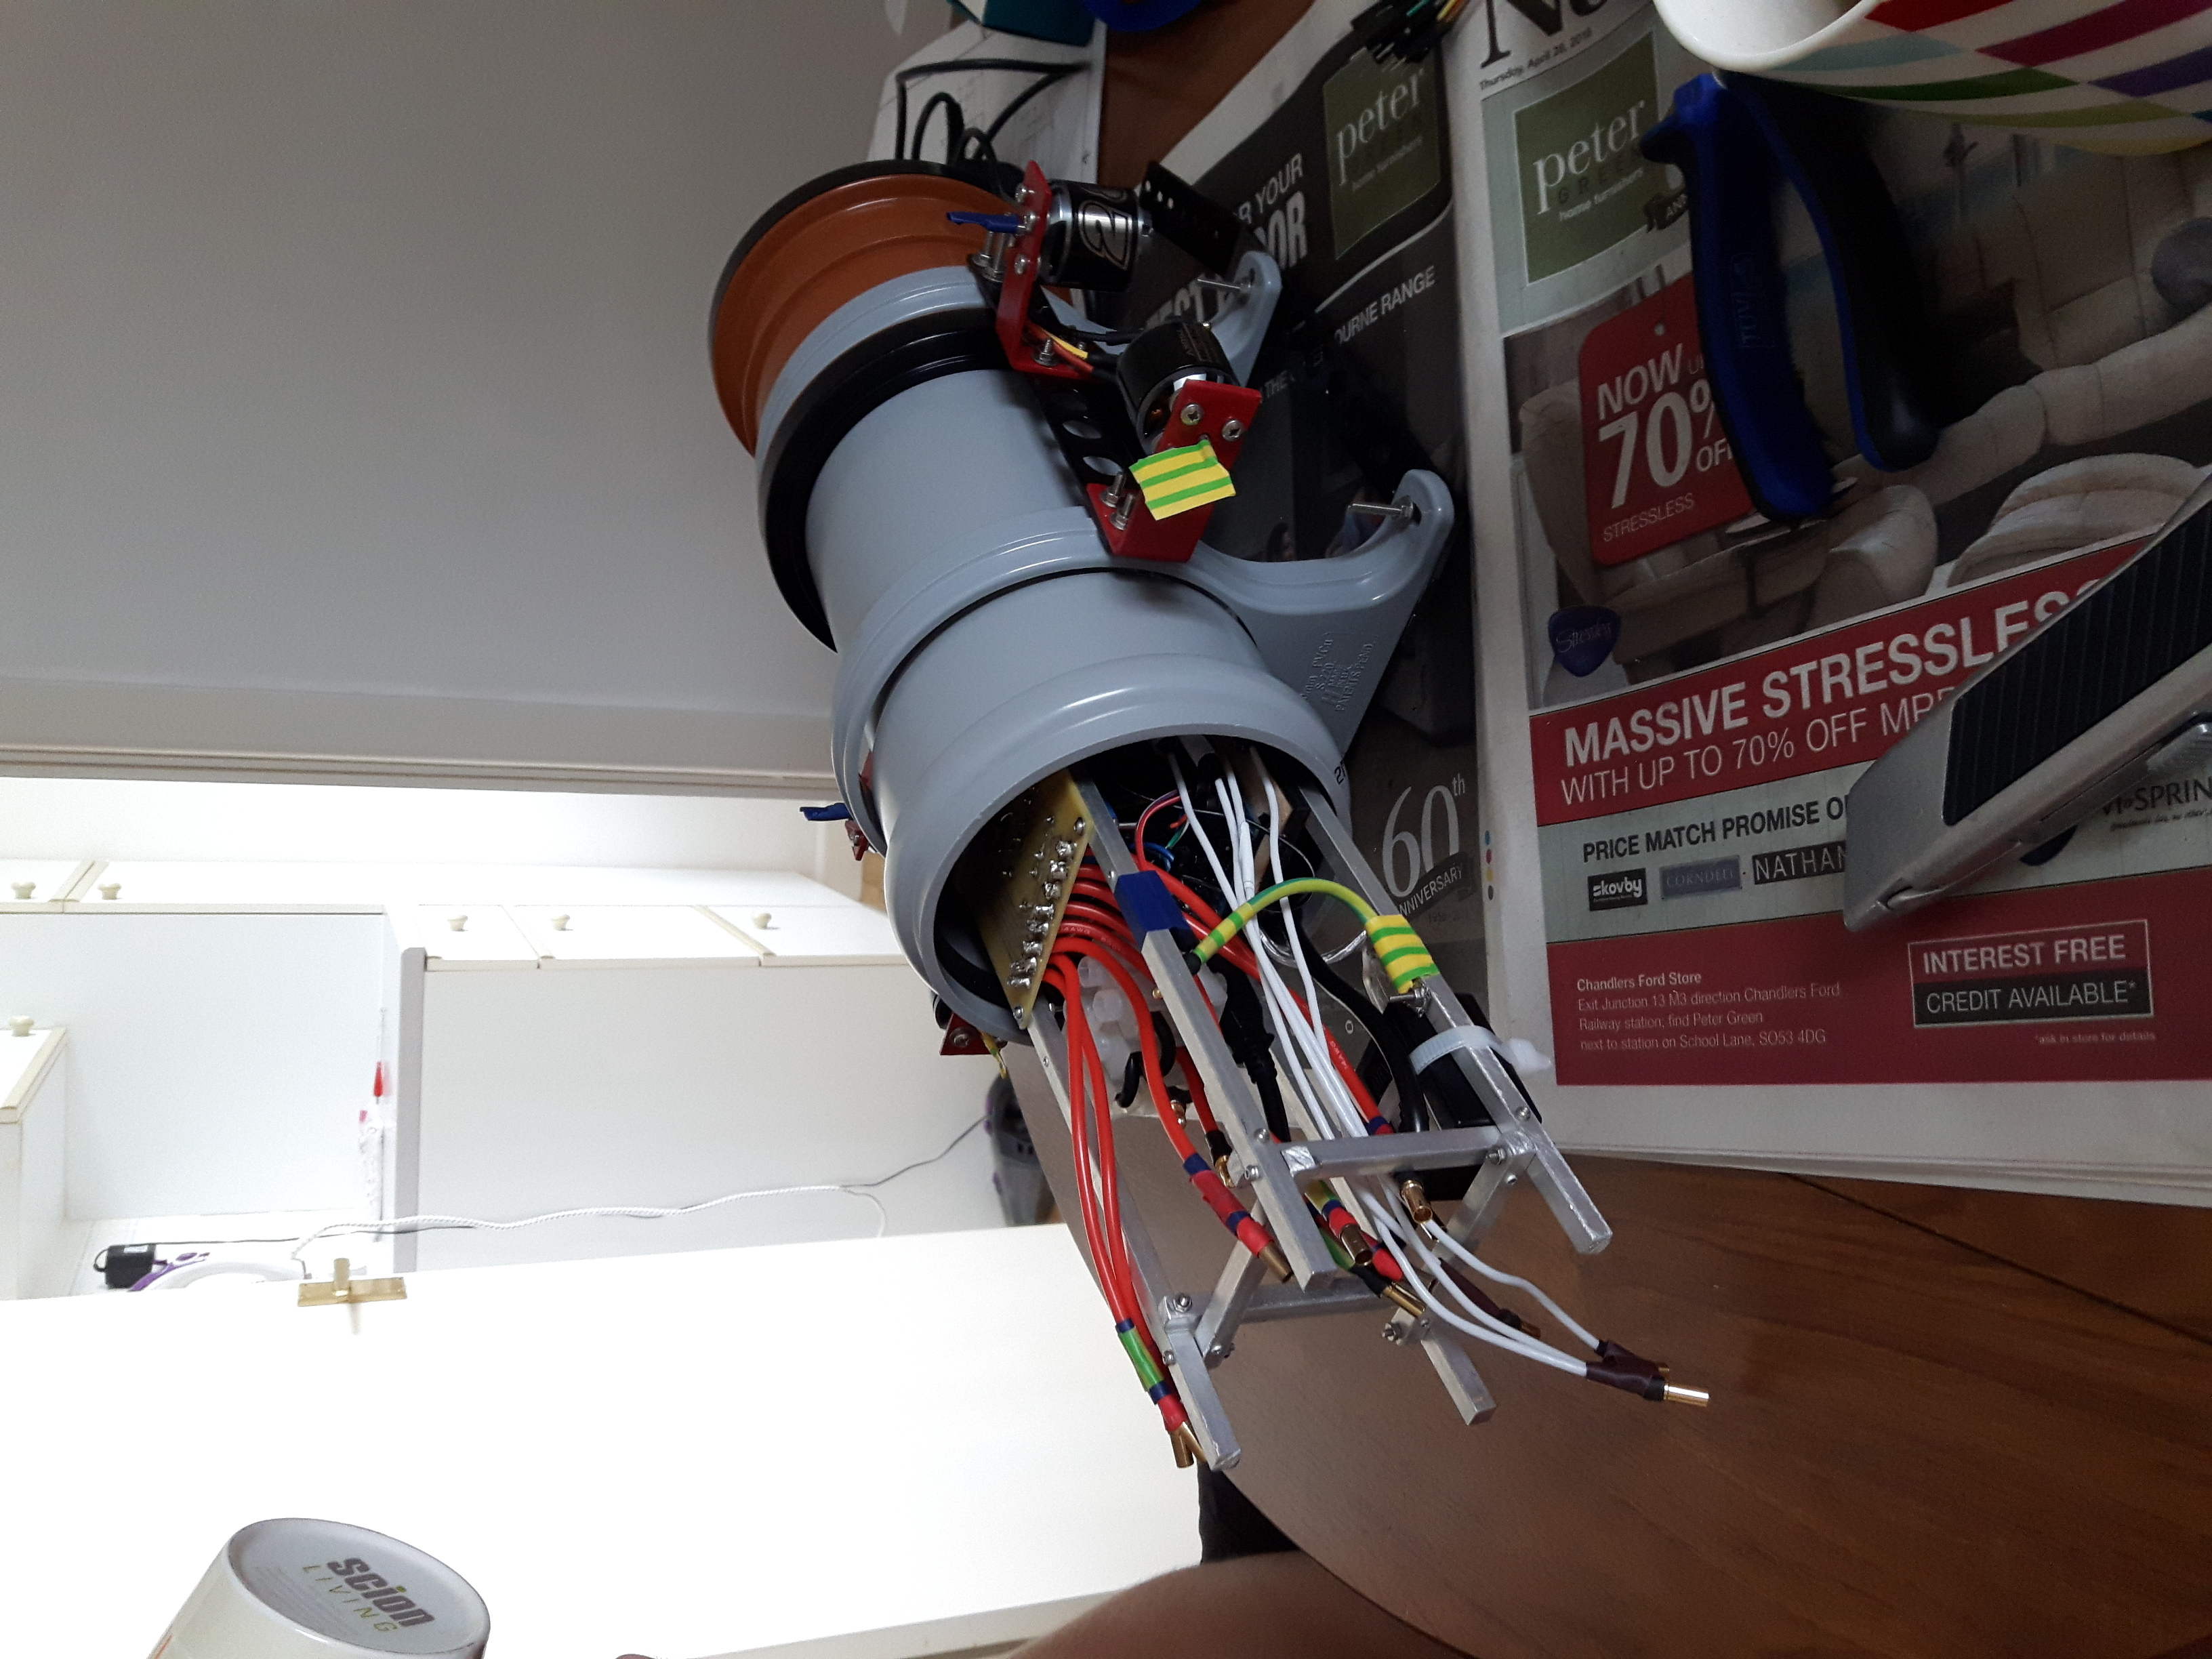
\includegraphics[width=\linewidth,angle=270]{20160625_145830.jpg}
\end{minipage}
\caption{Electronics are mounted to the internal aluminium structure, which slides into the pressure vessel.}
\label{fig:electronicsSlideIn}
\end{figure}

\begin{figure}[htb]
\begin{minipage}[b]{1\linewidth}
  \centering
	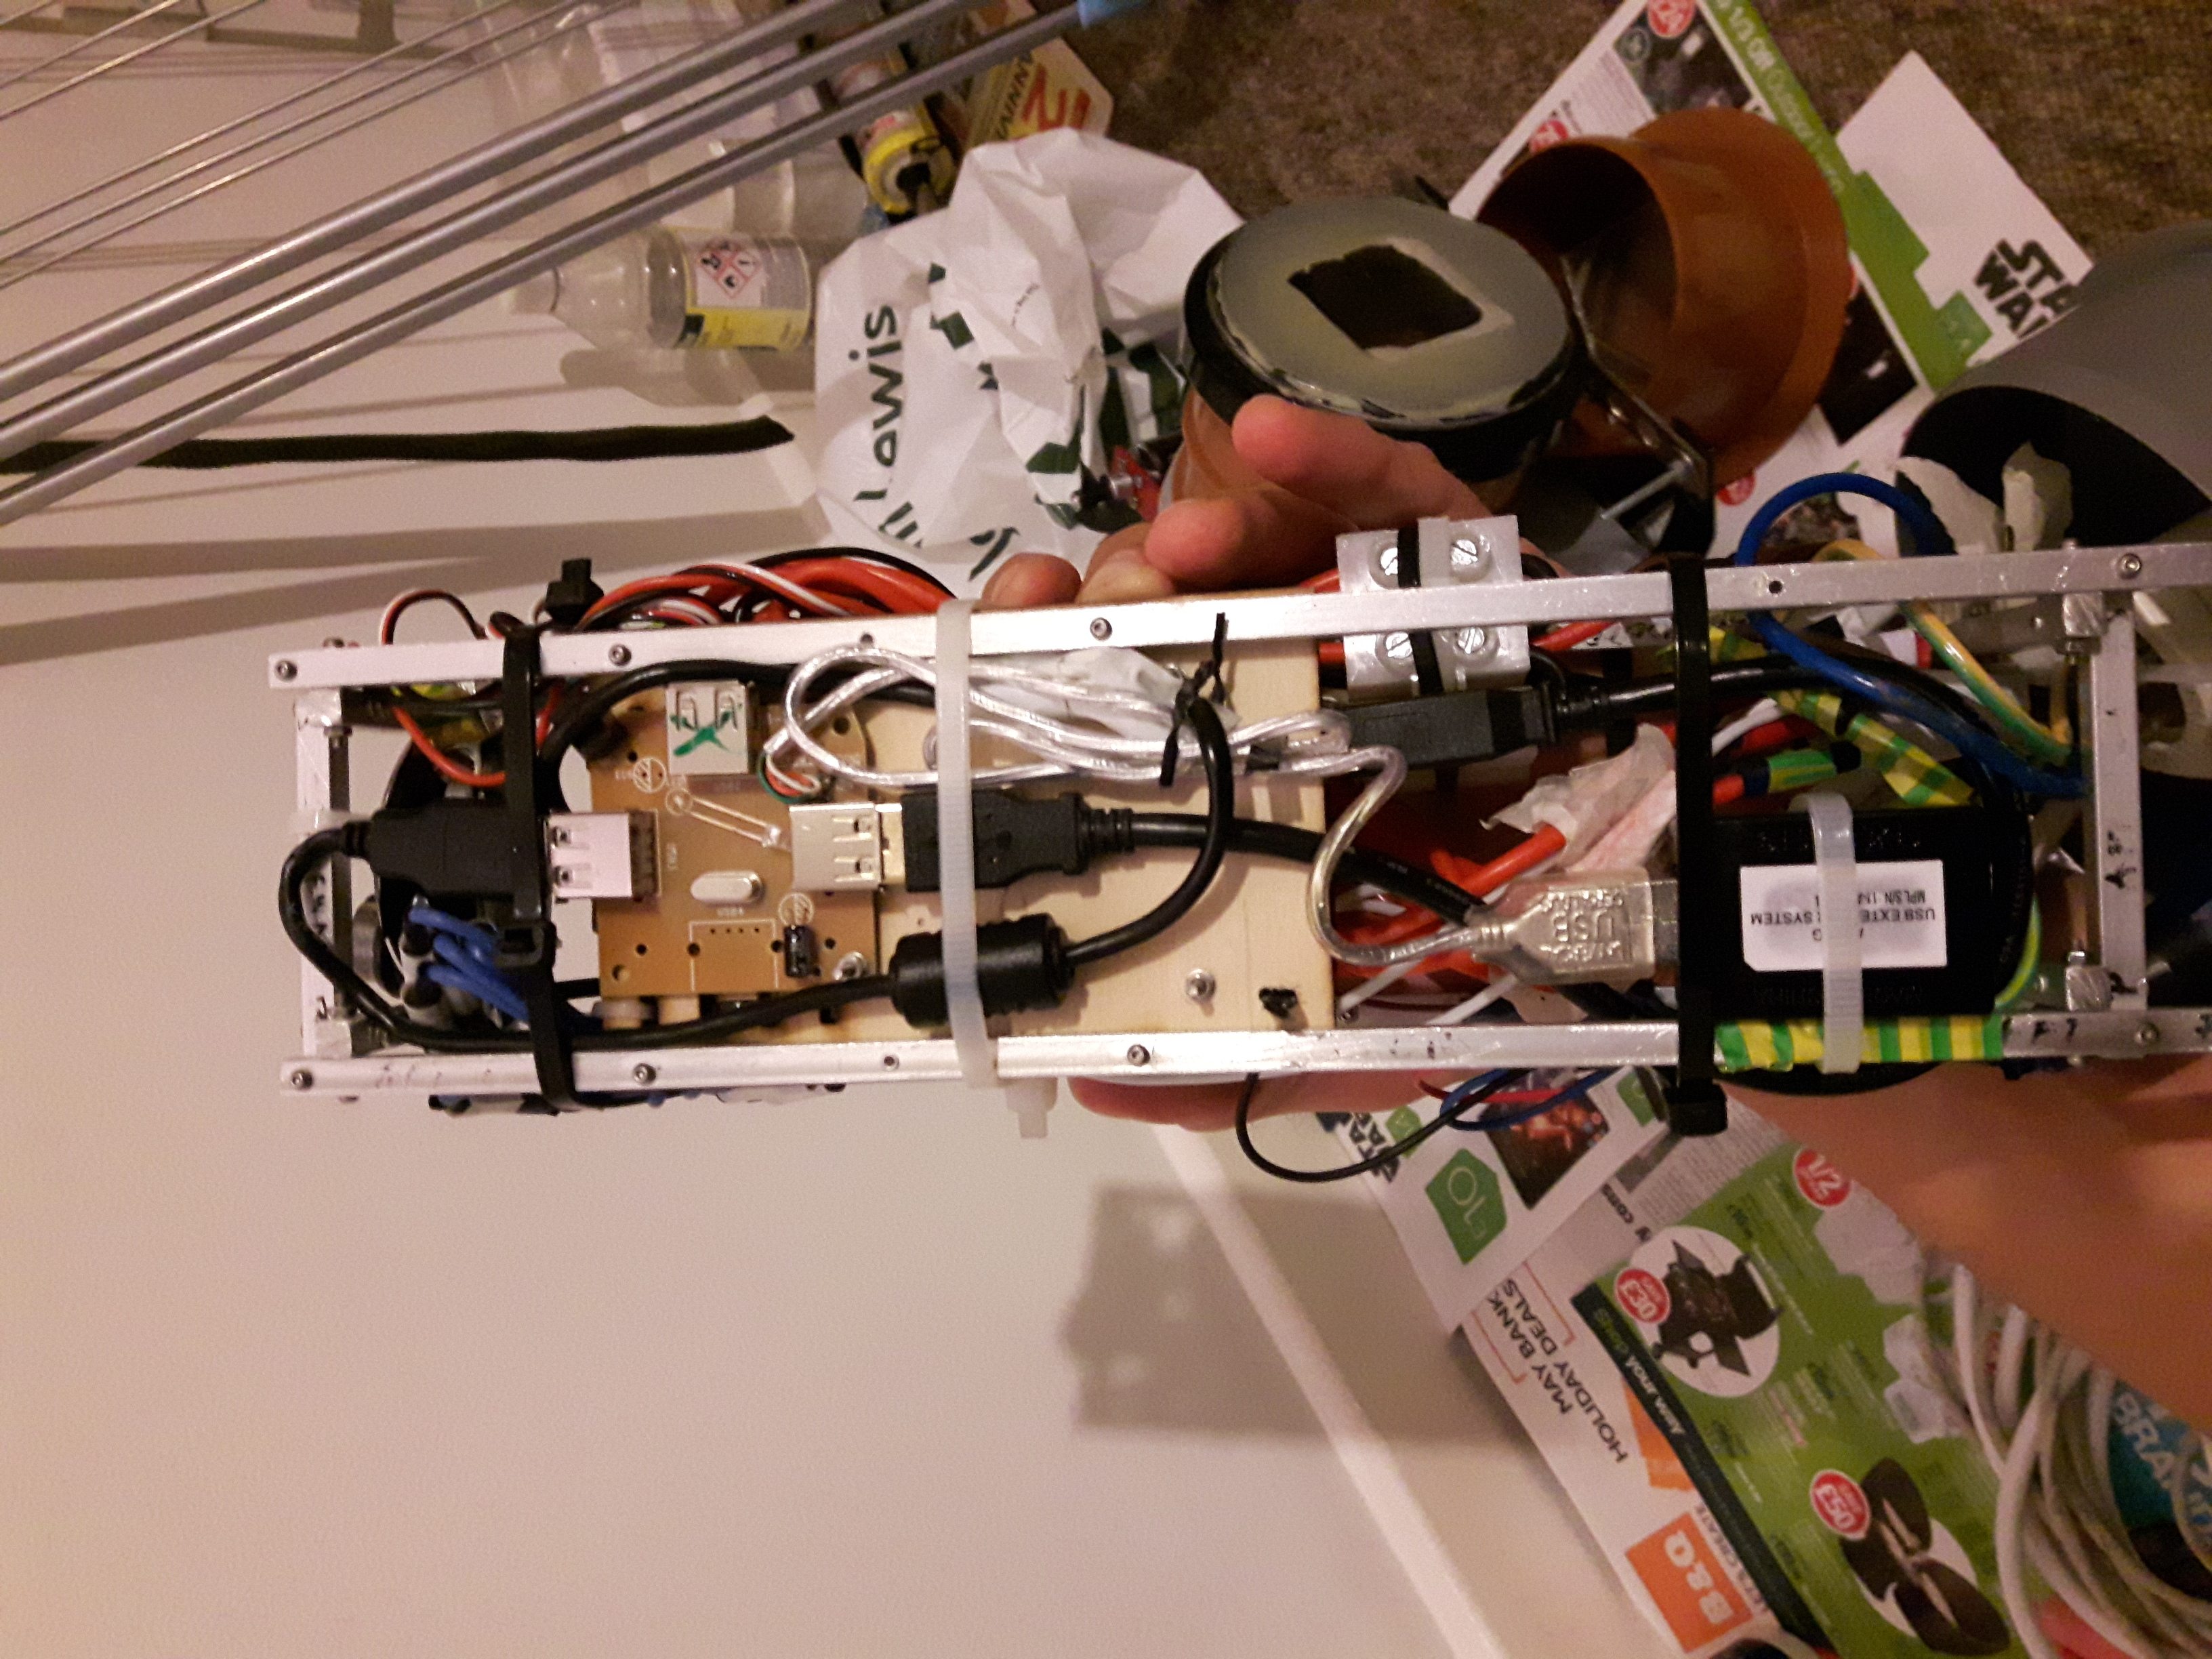
\includegraphics[width=\linewidth,angle=270]{20160826_213537.jpg}
\end{minipage}
\caption{USB range extender (black box on the bottom left of the phot) is mounted to the aluminium internal structure with a~white cable tie. The USB hub, into which Arduino and the webcam are plugged in, is bolted onto the underside of the plywood bed.}
\label{fig:usbExtenderAndHub}
\end{figure}

\begin{figure}[htb]
\begin{minipage}[b]{1\linewidth}
  \centering
	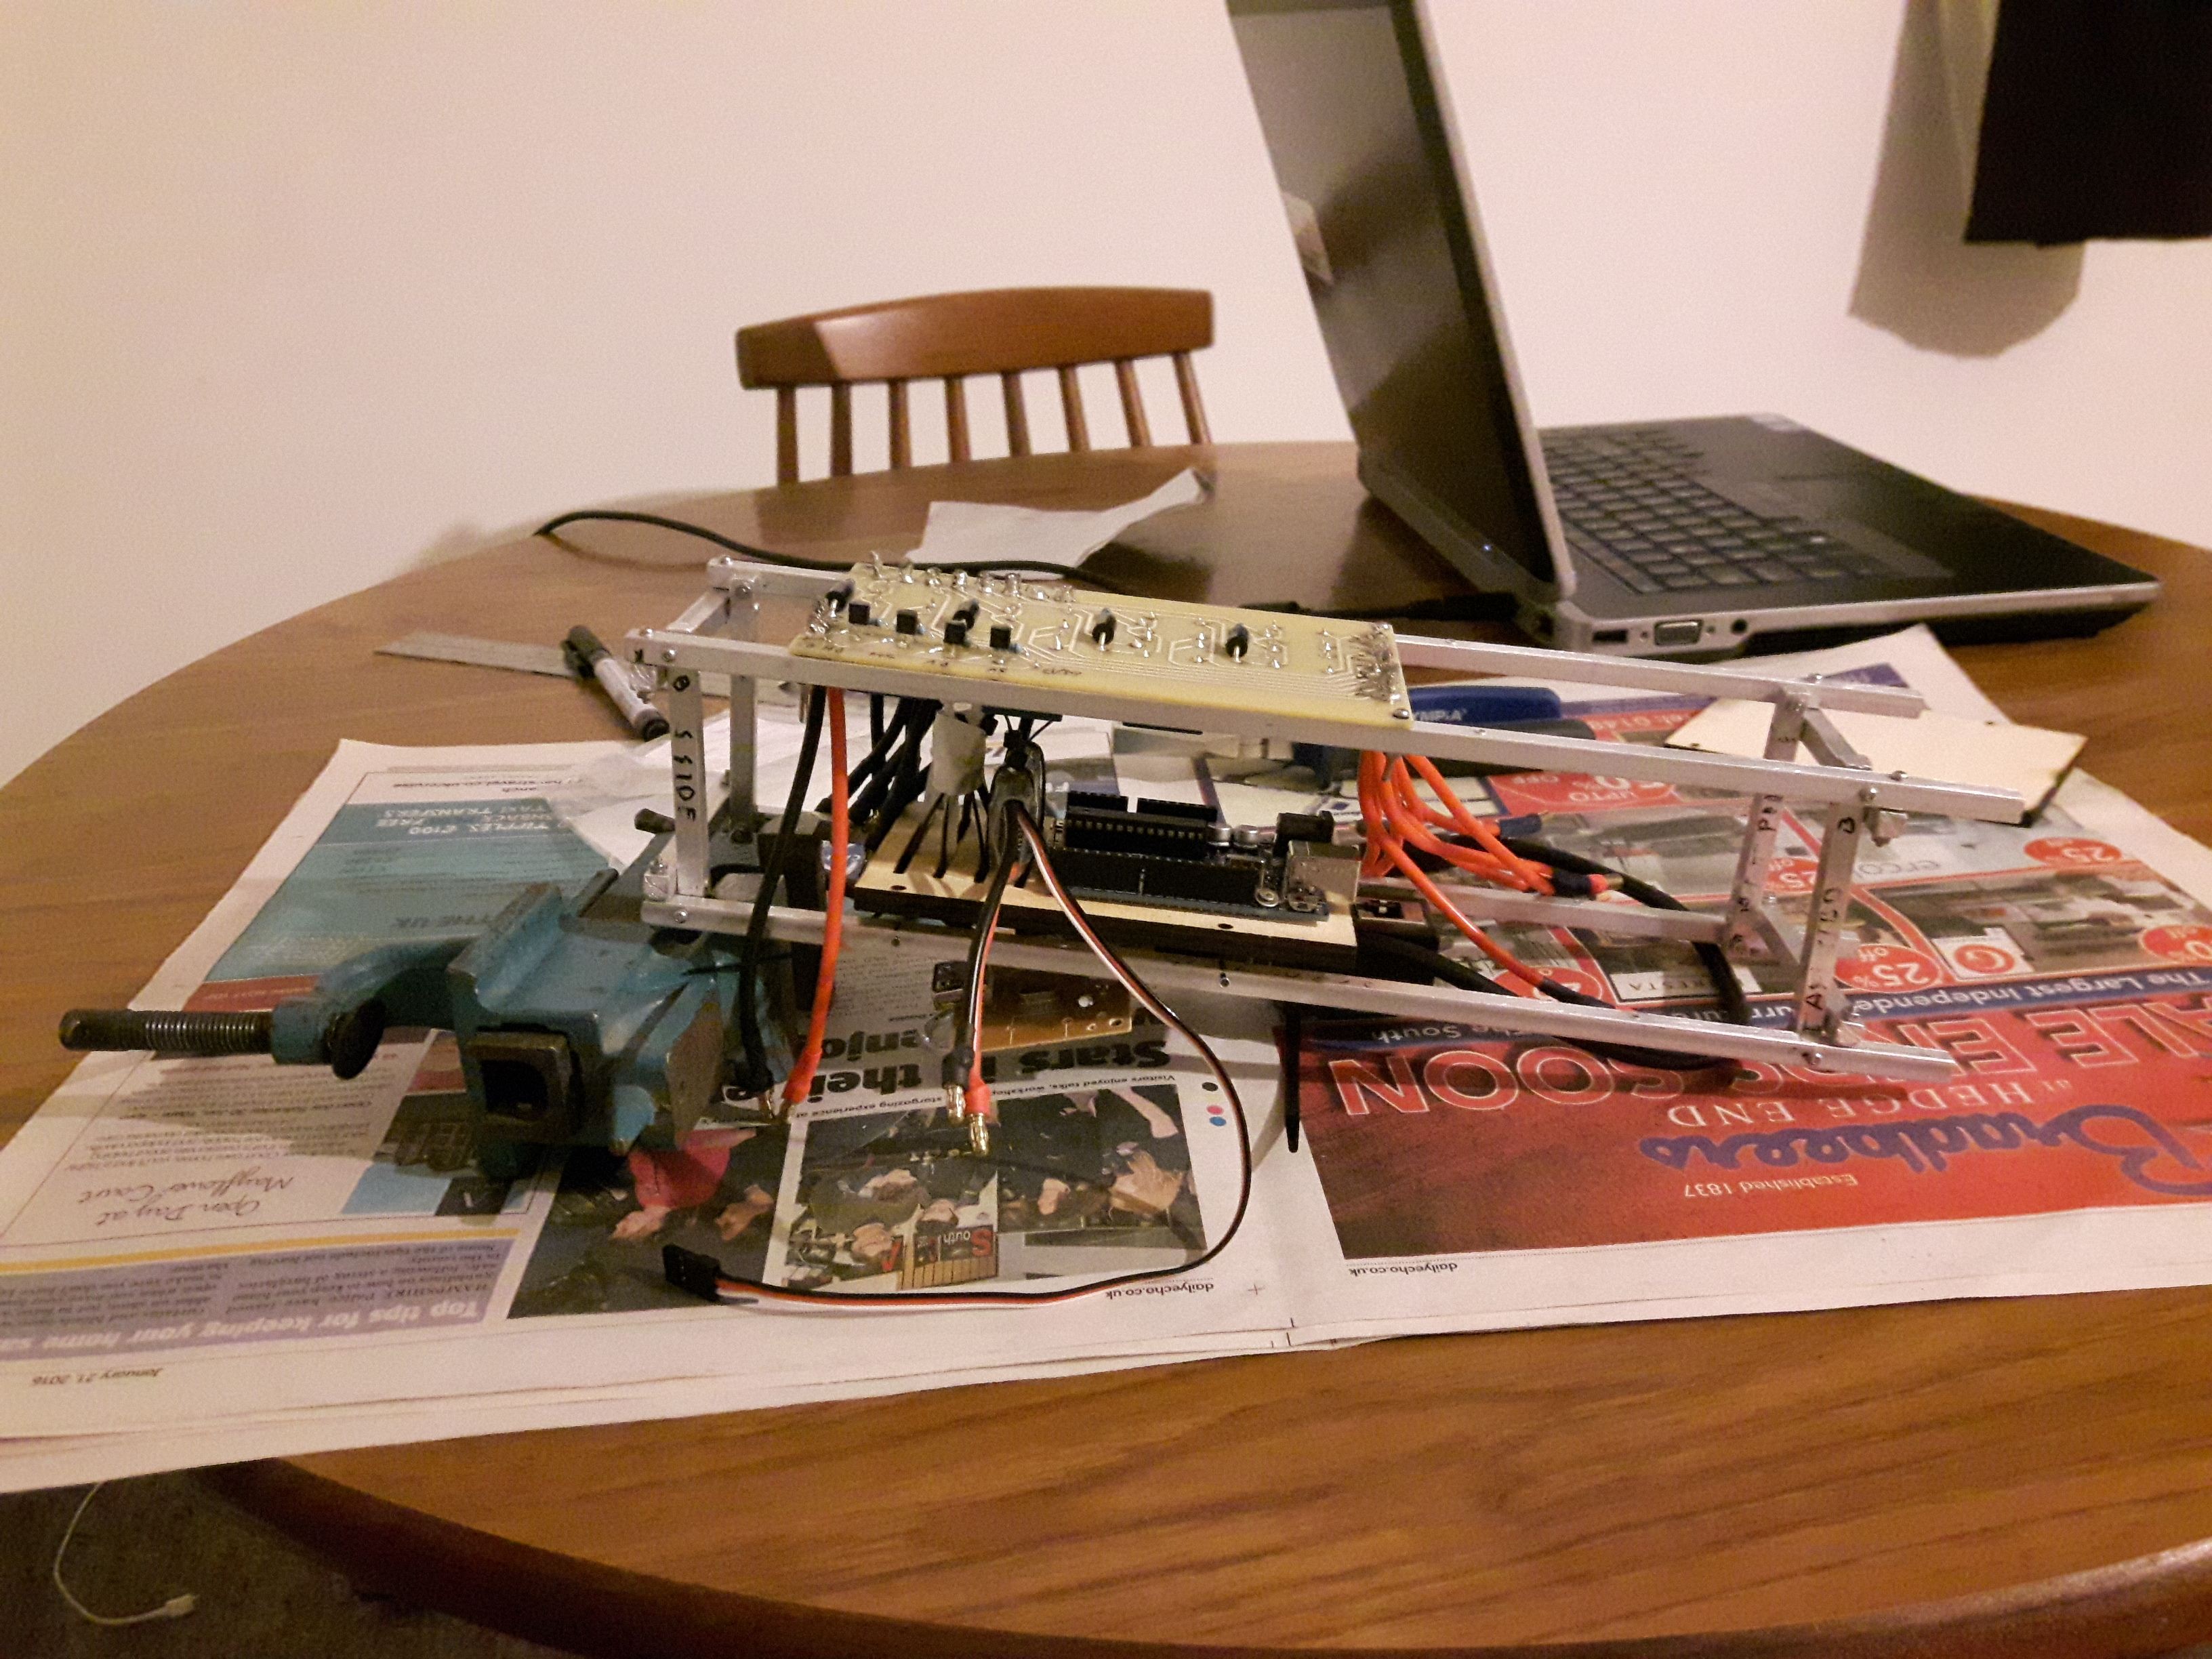
\includegraphics[width=\linewidth]{20160518_223426.jpg}
\end{minipage}
\caption{General arrangement of the internal electronics. Only one electronic speed controller, and no LEDs and camera are mounted for clarity.}
\label{fig:simpleInternalOverview}
\end{figure}

\clearpage % Place these figures close to the text.

%-------------------------------------------------------------------------------
\subsection{Power distribution subsystem}\label{ssection:powerDsitrbution}
Block diagram of the on-board power distribution subsystem is shown in Fig.~\ref{fig:powerBlockDiagram}. The Arduino and the camera are powered directly from the USB bus delivered on board via the CAT5 cable, which forms part of the tether (c.f. section~\ref{section:umbilical}). The USB bus is changed from the CAT5 cable to a~standard USB cable using the USB range extender, and then split by the USB hub to deliver power to both the camera and the Arduino.

The pressure sensor is powered from the Arduino \unit[5]{V} pin. The LEDs are turned on by setting an Arduino pin high, which provides sufficient power for them to operate. Both the pressure sensor and the LEDs are connected to the Arduino ground, and connections to both peripherals are realised using hookup wires.

The power for the ESCs and the motor control board is delivered from the shore-based battery via the power cable, which constitutes part of the tether. Custom power distribution unit (PDU) and common ground for these five components were manufactured out of automotive cable connectors. These components are shown in Fig.~\ref{fig:commonGround}; they connect the ESCs and the motor control board in parallel.

The ground (GND) of the Arduino is connected to four ESCs. However, these connections are separate from the ones that deliver power to the ESCs (negative battery terminals). Whether the Arduino GND and and battery GND are connected via the ESCs is unknown. The motor control board connects the Arduino and battery GND, as described in section~\ref{ssection:motorControlBoard}.

Power is delivered to the ESCs and motor control board using gauge 32 wires (thick lines in Fig.~\ref{fig:powerBlockDiagram}). All other connections in Fig.~\ref{fig:powerBlockDiagram} are realised using hookup wires.

The third wire in the power cable (besides battery positive and negative terminals) is used to ground the internal structure. This is intended to protect the operators in case the battery positive terminal short-circuits to one of the internal components or the aluminium structure. The external structure is not grounded.

The shore battery pack constitutes two \unit[6]{V} batteries connected in series. These are housed inside an aluminium box, which also incorporates a~\unit[20]{mm} fuse, switches and leads that can be used to monitor the battery voltage. Disassembled battery pack is shown in Fig.~\ref{fig:batteryPack}.

\begin{figure}[htb]
\begin{minipage}[b]{1\linewidth}
  \centering
	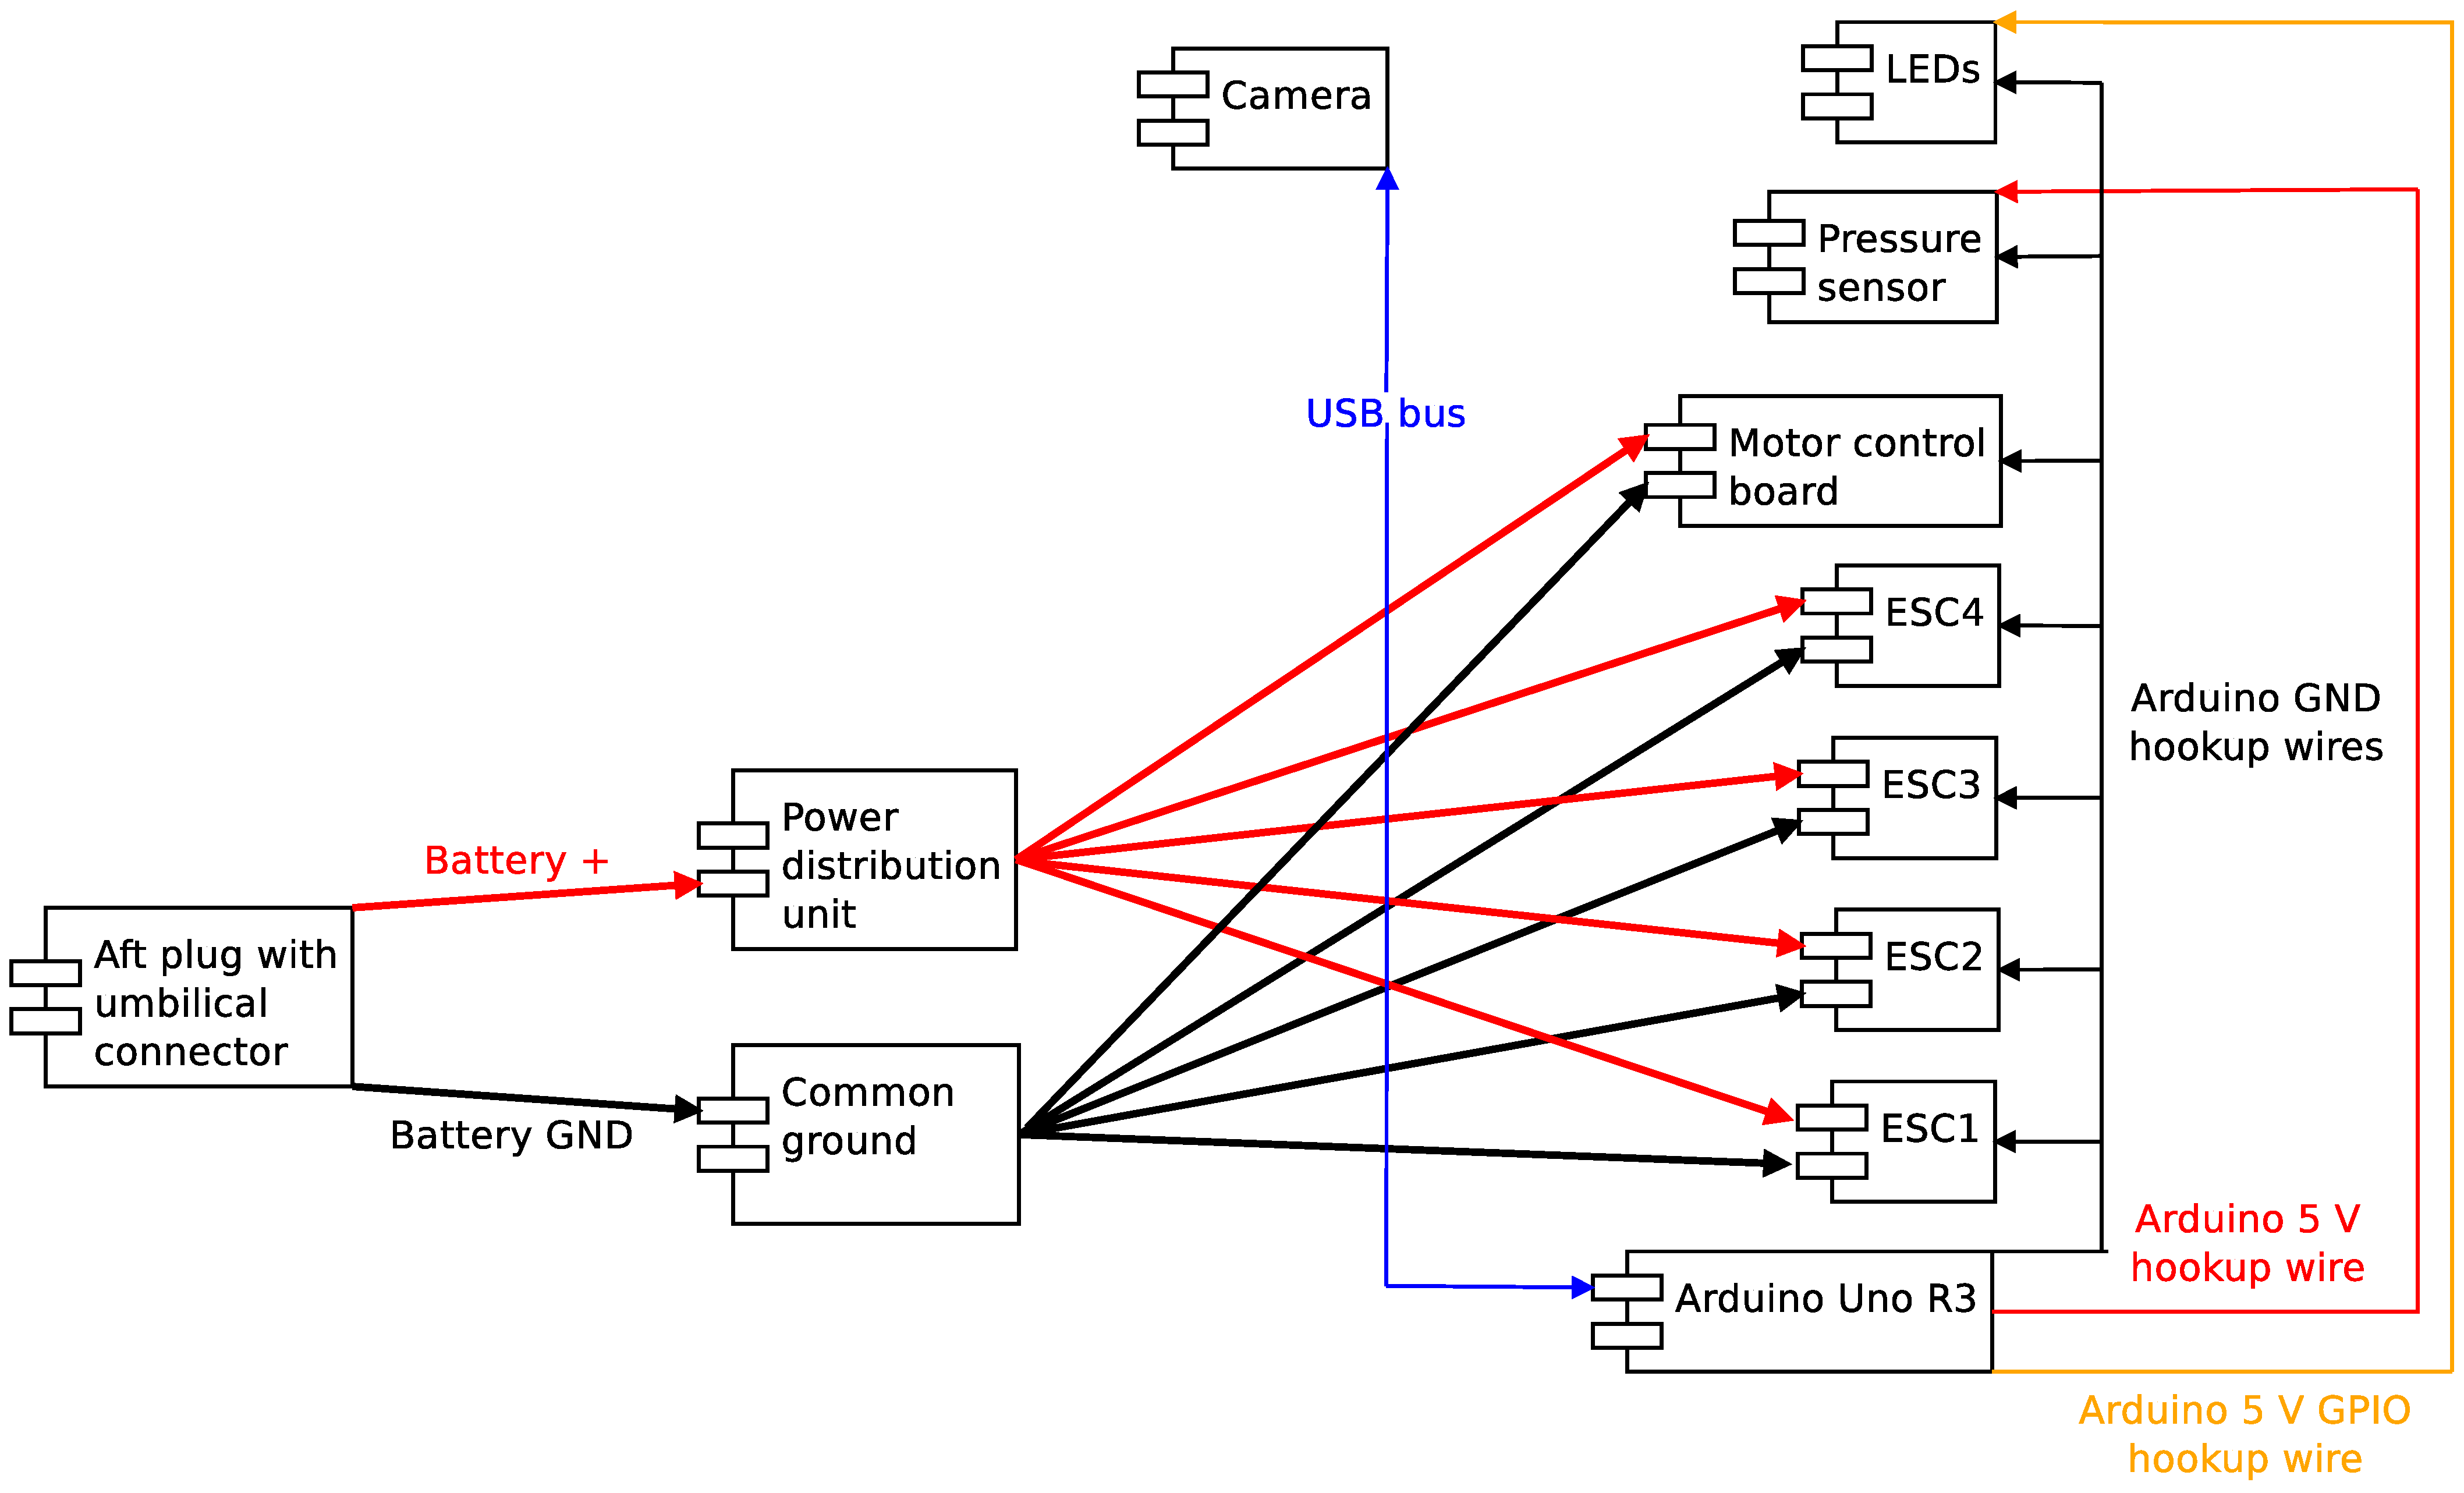
\includegraphics[width=1\linewidth,angle=90]{powerBlockDiagram.eps}
\end{minipage}
\caption{Block diagram of the power distribution subsystem. Power is delivered to the aft plug using the umbilical tether, which is connected to the battery pack.}
\label{fig:powerBlockDiagram}
\end{figure}

\begin{figure}[htb]
\begin{center}
\begin{tabular}{c c}
	\subfloat[Side]
		{\includegraphics*[width=0.6\textwidth,angle=270]{20160826_213345.jpg}
		\label{fig:commonGround:label:a} } &
	\subfloat[Top]
		{\includegraphics*[width=0.6\textwidth,angle=270]{20160826_213835.jpg}
		\label{fig:commonGround:label:b} } \\
\end{tabular}
\end{center}
\caption{Side and top views of the common ground and common power lines made out of screw automotive cable connectors and mounted to the aluminium internal structure with cable ties.}
\label{fig:commonGround}
\end{figure}

\begin{figure}[htb]
\begin{minipage}[b]{1\linewidth}
  \centering
	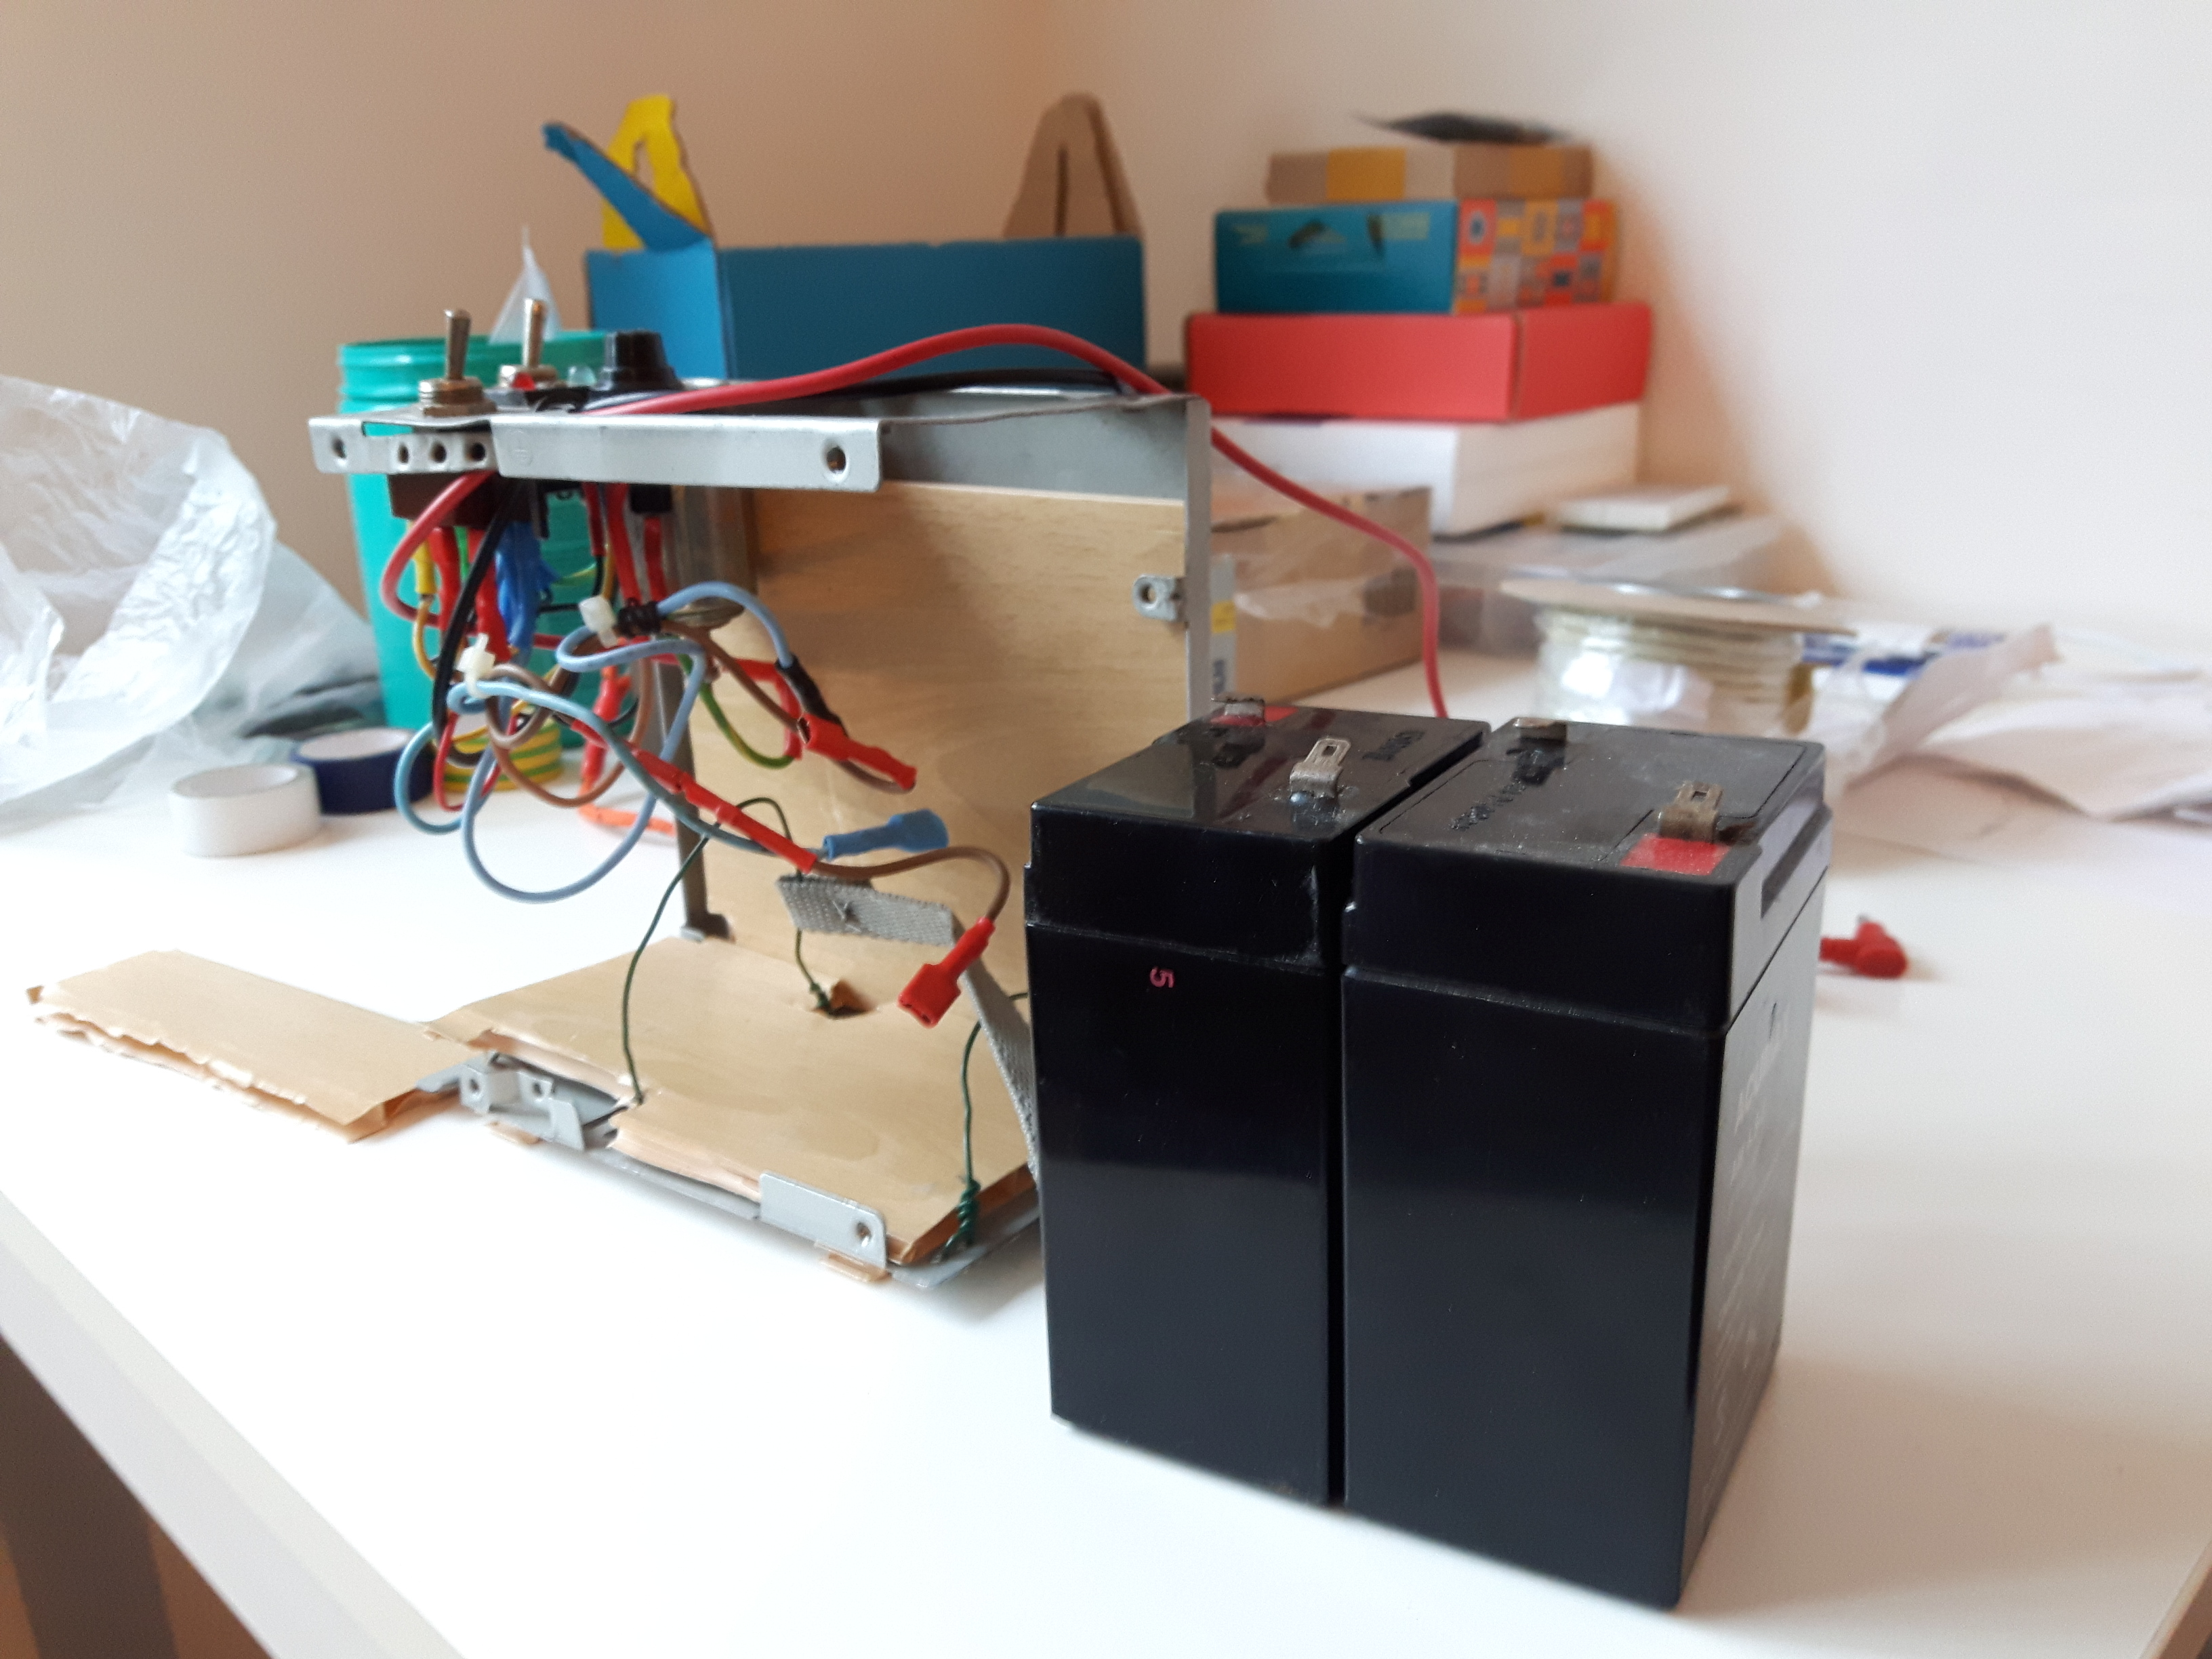
\includegraphics[width=1\linewidth]{20160828_184532.jpg}
\end{minipage}
\caption{Disassembled battery pack. One switch enables the batteries to be connected in parallel or in series (series configuration is used for the ROV project) while the other one switches the power on or off. The output of the battery pack is protected from excessive currents using a~\unit[20]{mm} fuse.}
\label{fig:batteryPack}
\end{figure}

\clearpage % Place these figures close to the text.

%-------------------------------------------------------------------------------
\subsection{Propulsion subsystem}\label{ssection:propulsionSubsystem}
Block diagram of the ROV propulsion subsystem is shown in Fig.~\ref{fig:propulsionBlockDiagram}. It is based on four brushless DC motors that are driven by four commercial, off-the-shelf electronic speed controllers. Every ESC converts a~pulse width modulation signal (PWM) from the Arduino into pulses of power delivered to every of three terminals on the brushless motor. Changing the frequency of the PWM changes the frequency of the power pulses, which changes the rotation frequency of the motor and so also its thrust. This PWM signal is delivered from the Arduino pins using hookup wires. The ESCs draw power, which is then delivered to the motors in pulses, directly from the shore-based batteries, which is described in section~\ref{ssection:powerDsitrbution}.

In order to reverse thrust of the motor, it suffices to swap two out of three signals output by the ESC. This is achieved by a~custom printed circuit board, which is described in more detail in section~\ref{ssection:motorControlBoard}. Two out of three outputs of every ESC (terminals 1 and 2 in Fig.~\ref{fig:propulsionBlockDiagram}) are routed through this board, before they are delivered to the corresponding motors using the connector in the aft plug using red wires in Fig.~\ref{fig:electronicsSlideIn}. The third signal of every ESC (terminal 3 in Fig.~\ref{fig:propulsionBlockDiagram}) circumvents the motor control board and connects to the corresponding motor only through the connector in the aft plug (white wires in Fig.~\ref{fig:electronicsSlideIn}). The commands to swap the thrust of a~given motor are issued to the motor control board via hookup wires connected to the Arduino pins.

The ESCs are mounted to the plywood bed ahead of the Arduino using cable ties (the aft-most ESC is visible in Fig.~\ref{fig:simpleInternalOverview}). The ESCs connect to the motor control board, the aft plug connector, and the motors using gauge 32 wires.

\begin{figure}[htb]
\begin{minipage}[b]{1\linewidth}
  \centering
	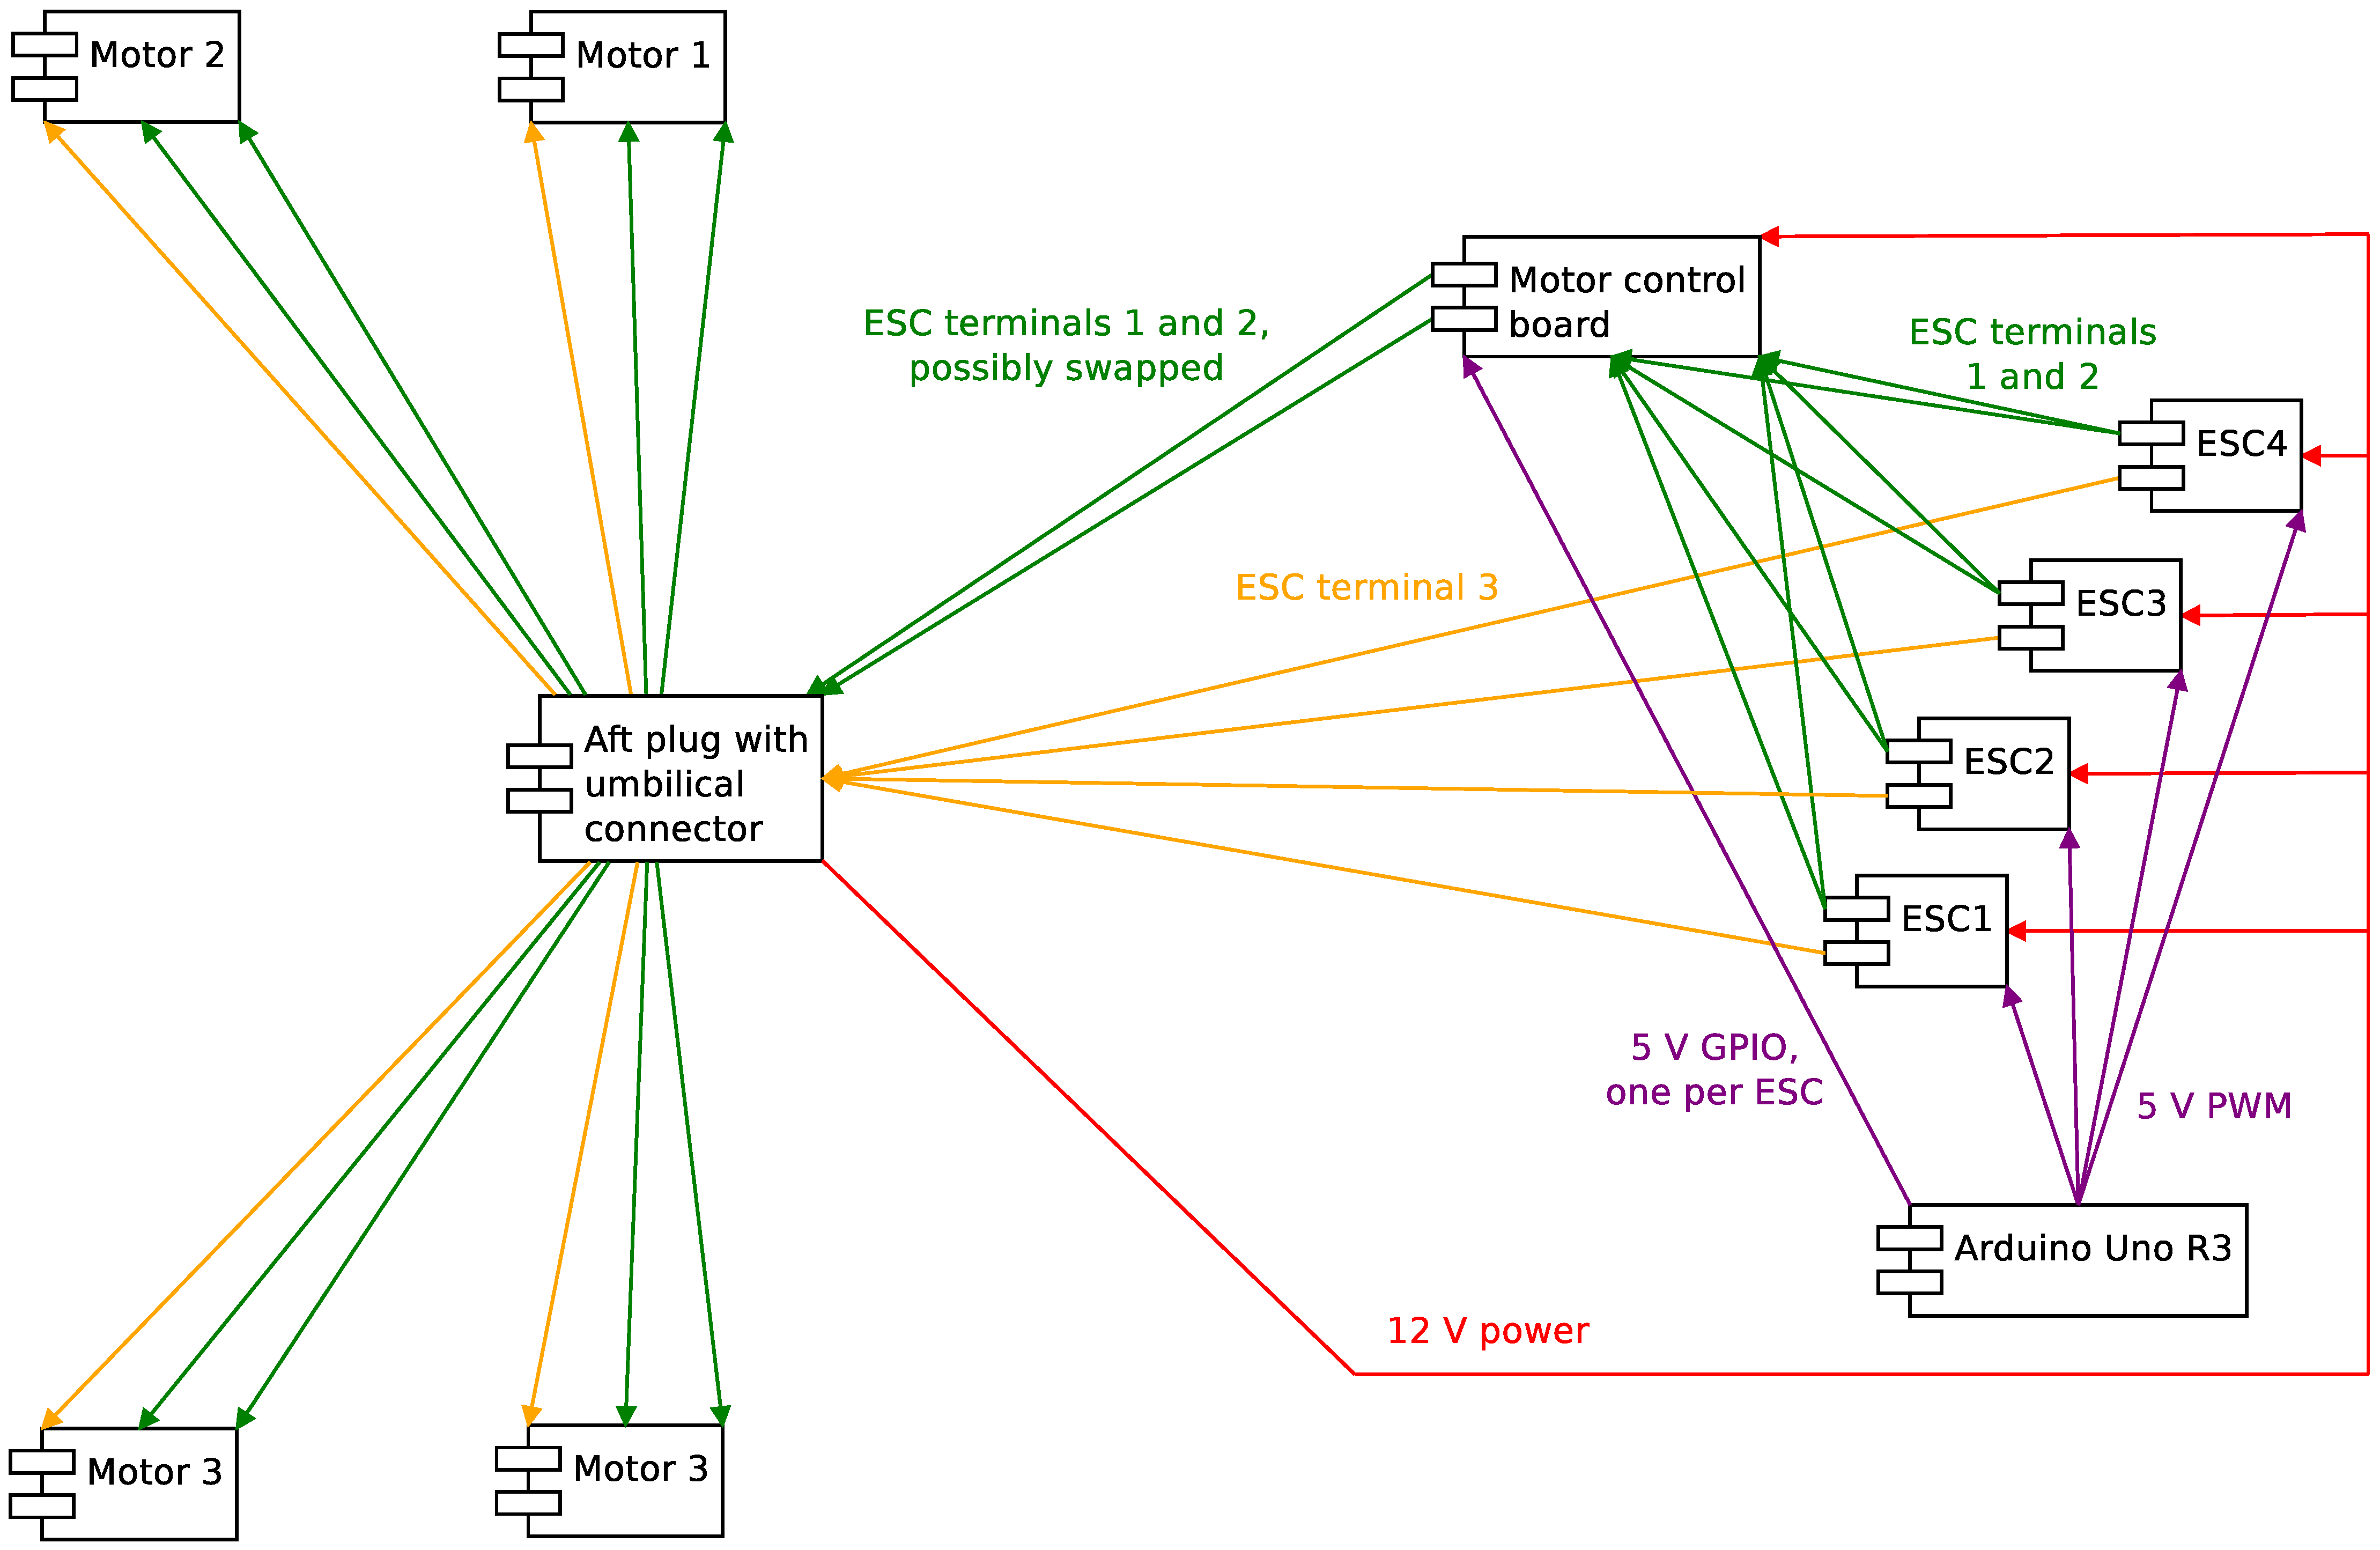
\includegraphics[width=1\linewidth,angle=90]{propulsionBlockDiagram.eps}
\end{minipage}
\caption{Block diagram of the ROV propulsion subsystem. \textcolor{purple}{Connections from the Arduino} are realised using hookup wires. All other signals (\textcolor{red}{power}, and ESC signals \textcolor{green}{1, 2} and \textcolor{orange}{3}) are carried using gauge 32 wire.}
\label{fig:propulsionBlockDiagram}
\end{figure}

%-------------------------------------------------------------------------------
\subsection{Brushless-motor control board}\label{ssection:motorControlBoard}
As explained in section~\ref{ssection:propulsionSubsystem}, two signals from every ESC have to be swapped in order to reverse the thrust of a~motor. The schematic of the circuit, which achieves this, is shown in Fig.~\ref{fig:motorControlBoardSchematic}. Nominally, terminals 1 and 2 of every ESC (e.g. ESC1T1 and ESC1T2 for ESC no.~1) are connected to terminals 1 and 2 of the corresponding motor (e.g. M1T1 and M1T2 for motor no.~1). When a~command to reverse the thrust of a~given motor is issued by the Arduino by setting one of its pins high (e.g. pin~2 for motor no.~1), an n-type mosfet activates two switching relays. This connects terminals 1 and 2 of the ESC with terminals 2 and 1 of the motor, respectively, thus reversing the thrust. When the command pin is set low, the relays switch back to the nominal configuration and thrust is no longer reversed.

The power output of the Arduino is insufficient to activate the relays - relatively large relays, which can withstand currents output by the ESCs, have to be used. Thus, the power to the relays is delivered by the shore-based batteries. Every ESC-motor pair requires two switching relays, and every two relays have one flyback diode.

A~two-layer PCB houses the entire circuit from Fig.~\ref{fig:motorControlBoardSchematic}; its layout is shown in Fig.~\ref{fig:motorControlBoardLayout}. The motor control PCB is manufactured with 1 oz Cu and has trace widths of at least \unit[1]{mm} rated to at least \unit[2.5]{A}. The design of this board is open-source, and can be accessed in its repository at: \textcolor{blue}{\url{{www.upverter.com/AleksanderLidtke/7eccd1441d1097f8/BrushlessMotorControlBoard/}}}.

\begin{figure}[htb]
\begin{minipage}[b]{1\linewidth}
  \centering
	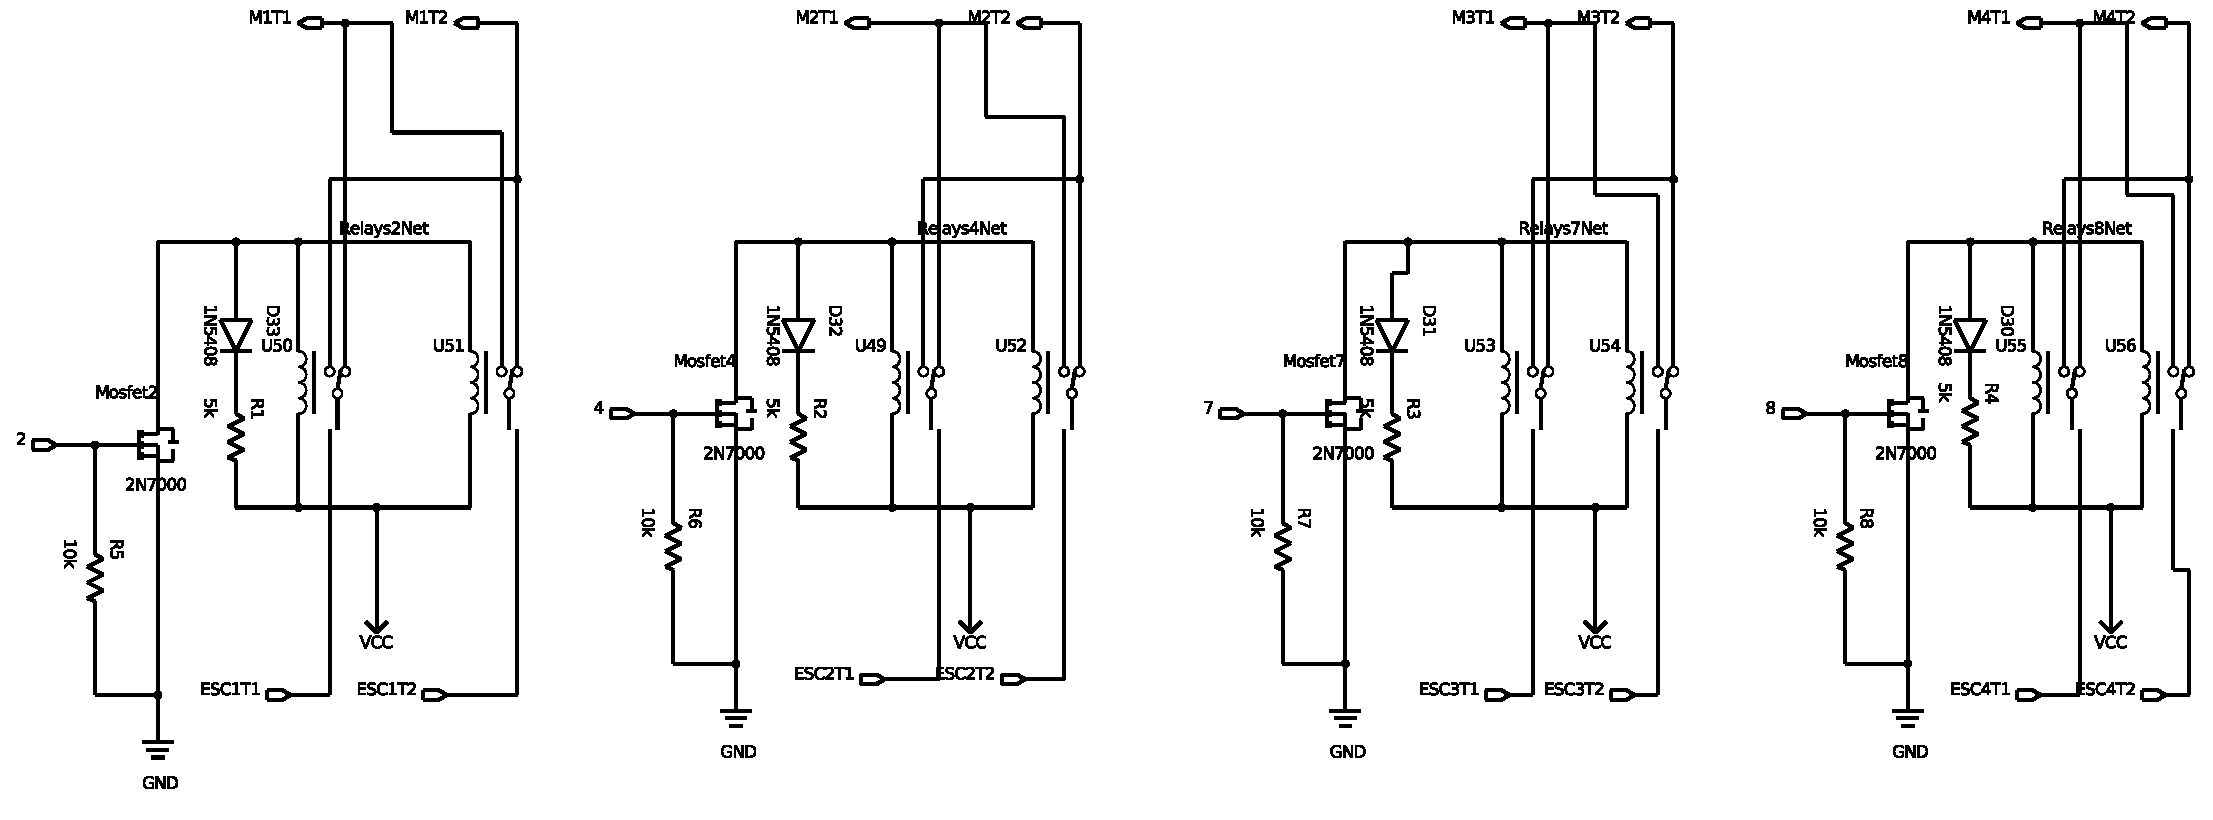
\includegraphics[width=1\linewidth,angle=90]{motorControlBoardSchematic.pdf}
\end{minipage}
\caption{Schematic of the brushless motor control PCB. The board connects terminals of ESCs to motor terminals via pairs of switching relays.}
\label{fig:motorControlBoardSchematic}
\end{figure}

\begin{figure}[htb]
\begin{minipage}[b]{1\linewidth}
  \centering
	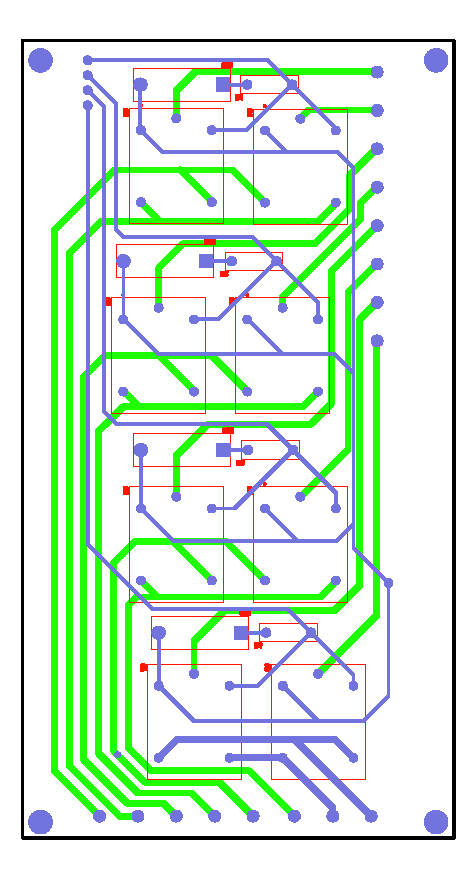
\includegraphics[width=0.75\linewidth]{motorControlBoardLayout.eps}
\end{minipage}
\caption{Layout of the brushless motor control PCB. Bottom copper marked with \textcolor{green}{green}, top with \textcolor{blue}{blue}, and component outlines with \textcolor{red}{red}. Switching relays are mounted on the top, and resistors, diodes and n-type mosfets on the bottom of the board. The PCB is actually mounted upside down in the vehicle, so that the bottom copper layer is facing the top of the ROV.}
\label{fig:motorControlBoardLayout}
\end{figure}

\clearpage % Place these figures close to the text.

%-------------------------------------------------------------------------------
\subsection{LEDs and camera}\label{ssection:ledAndCamera}
A~small, one-layer PCB, which houses three white LEDs connected in series, is mounted to a~reflective plastic surface. A~hole is drilled in the plastic, through which a~disassembled USB webcam is pointed in the direction of the LED lights. These LEDs and camera form a~stand-alone module, which is shown in Fig.~\ref{fig:forwardLED:label:a}. The module is mounted to the front of the internal aluminium frame of the ROV using cable ties, as shown in Fig.~\ref{fig:forwardLED:label:b}. A~translucent window is placed in the pressure vessel in front of the camera, which is described in section~\ref{ssection:forwardPlug}. As shown in Fig.~\ref{fig:powerBlockDiagram}, the LEDs are activated and powered directly from a~GPIO pin of the Arduino, whereas the camera is powered and operated via the USB bus.

\begin{figure}[htb]
\begin{center}
\begin{tabular}{c c}
	\subfloat[LED and camera module]
		{\includegraphics*[width=0.6\textwidth,angle=270]{20160319_174439.jpg}
		\label{fig:forwardLED:label:a} } &
	\subfloat[Module mounting]
		{\includegraphics*[width=0.6\textwidth,angle=270]{20160826_213436.jpg}
		\label{fig:forwardLED:label:b} } \\
\end{tabular}
\end{center}
\caption{The module, which houses the LEDs and the camera, and its mounting in the vehicle.}
\label{fig:forwardLED}
\end{figure}

%-------------------------------------------------------------------------------
\subsection{Pressure sensor}\label{ssection:pressureSensor}

A~\unit[30]{PSI} pressure transducer, depicted in Figure \ref{fig:pressureTransducer}, is mounted in the aft plug, which is a~modified PVC socket plug shown in Fig.~\ref{fig:socketPlug}. A~hole was punched in the socket plug, into which the pressure sensor was screwed in. The connection was sealed by applying PTFE tape on the thread of the pressure transducer and inserting rubber washers on either side of the socket plug. The entire assembly was then tightened using a~nut and a~washer placed on the external side of the socket plug. The inlet of the pressure sensor, brass nut and a~steel washer, under which a~rubber washer is placed, can be seen in Fig.~\ref{fig:externalSideOfTheAftPlug}. The transducer is powered from the Arduino \unit[5]{V} pin through a~hookup wire. It is connected to the Arduino GND and an analogue input pin using hookup wires as well.

\begin{figure}[htb]
\centering
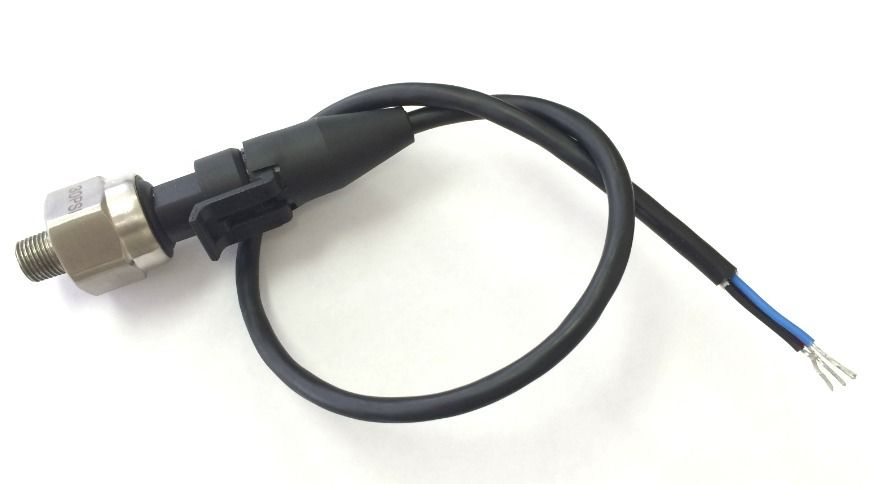
\includegraphics[width=0.8\linewidth]{pressureTransducer.jpg}
\caption{Overview of the pressure transducer.}
\label{fig:pressureTransducer}
\end{figure}

\begin{figure}[htb]
\begin{minipage}[b]{1\linewidth}
  \centering
	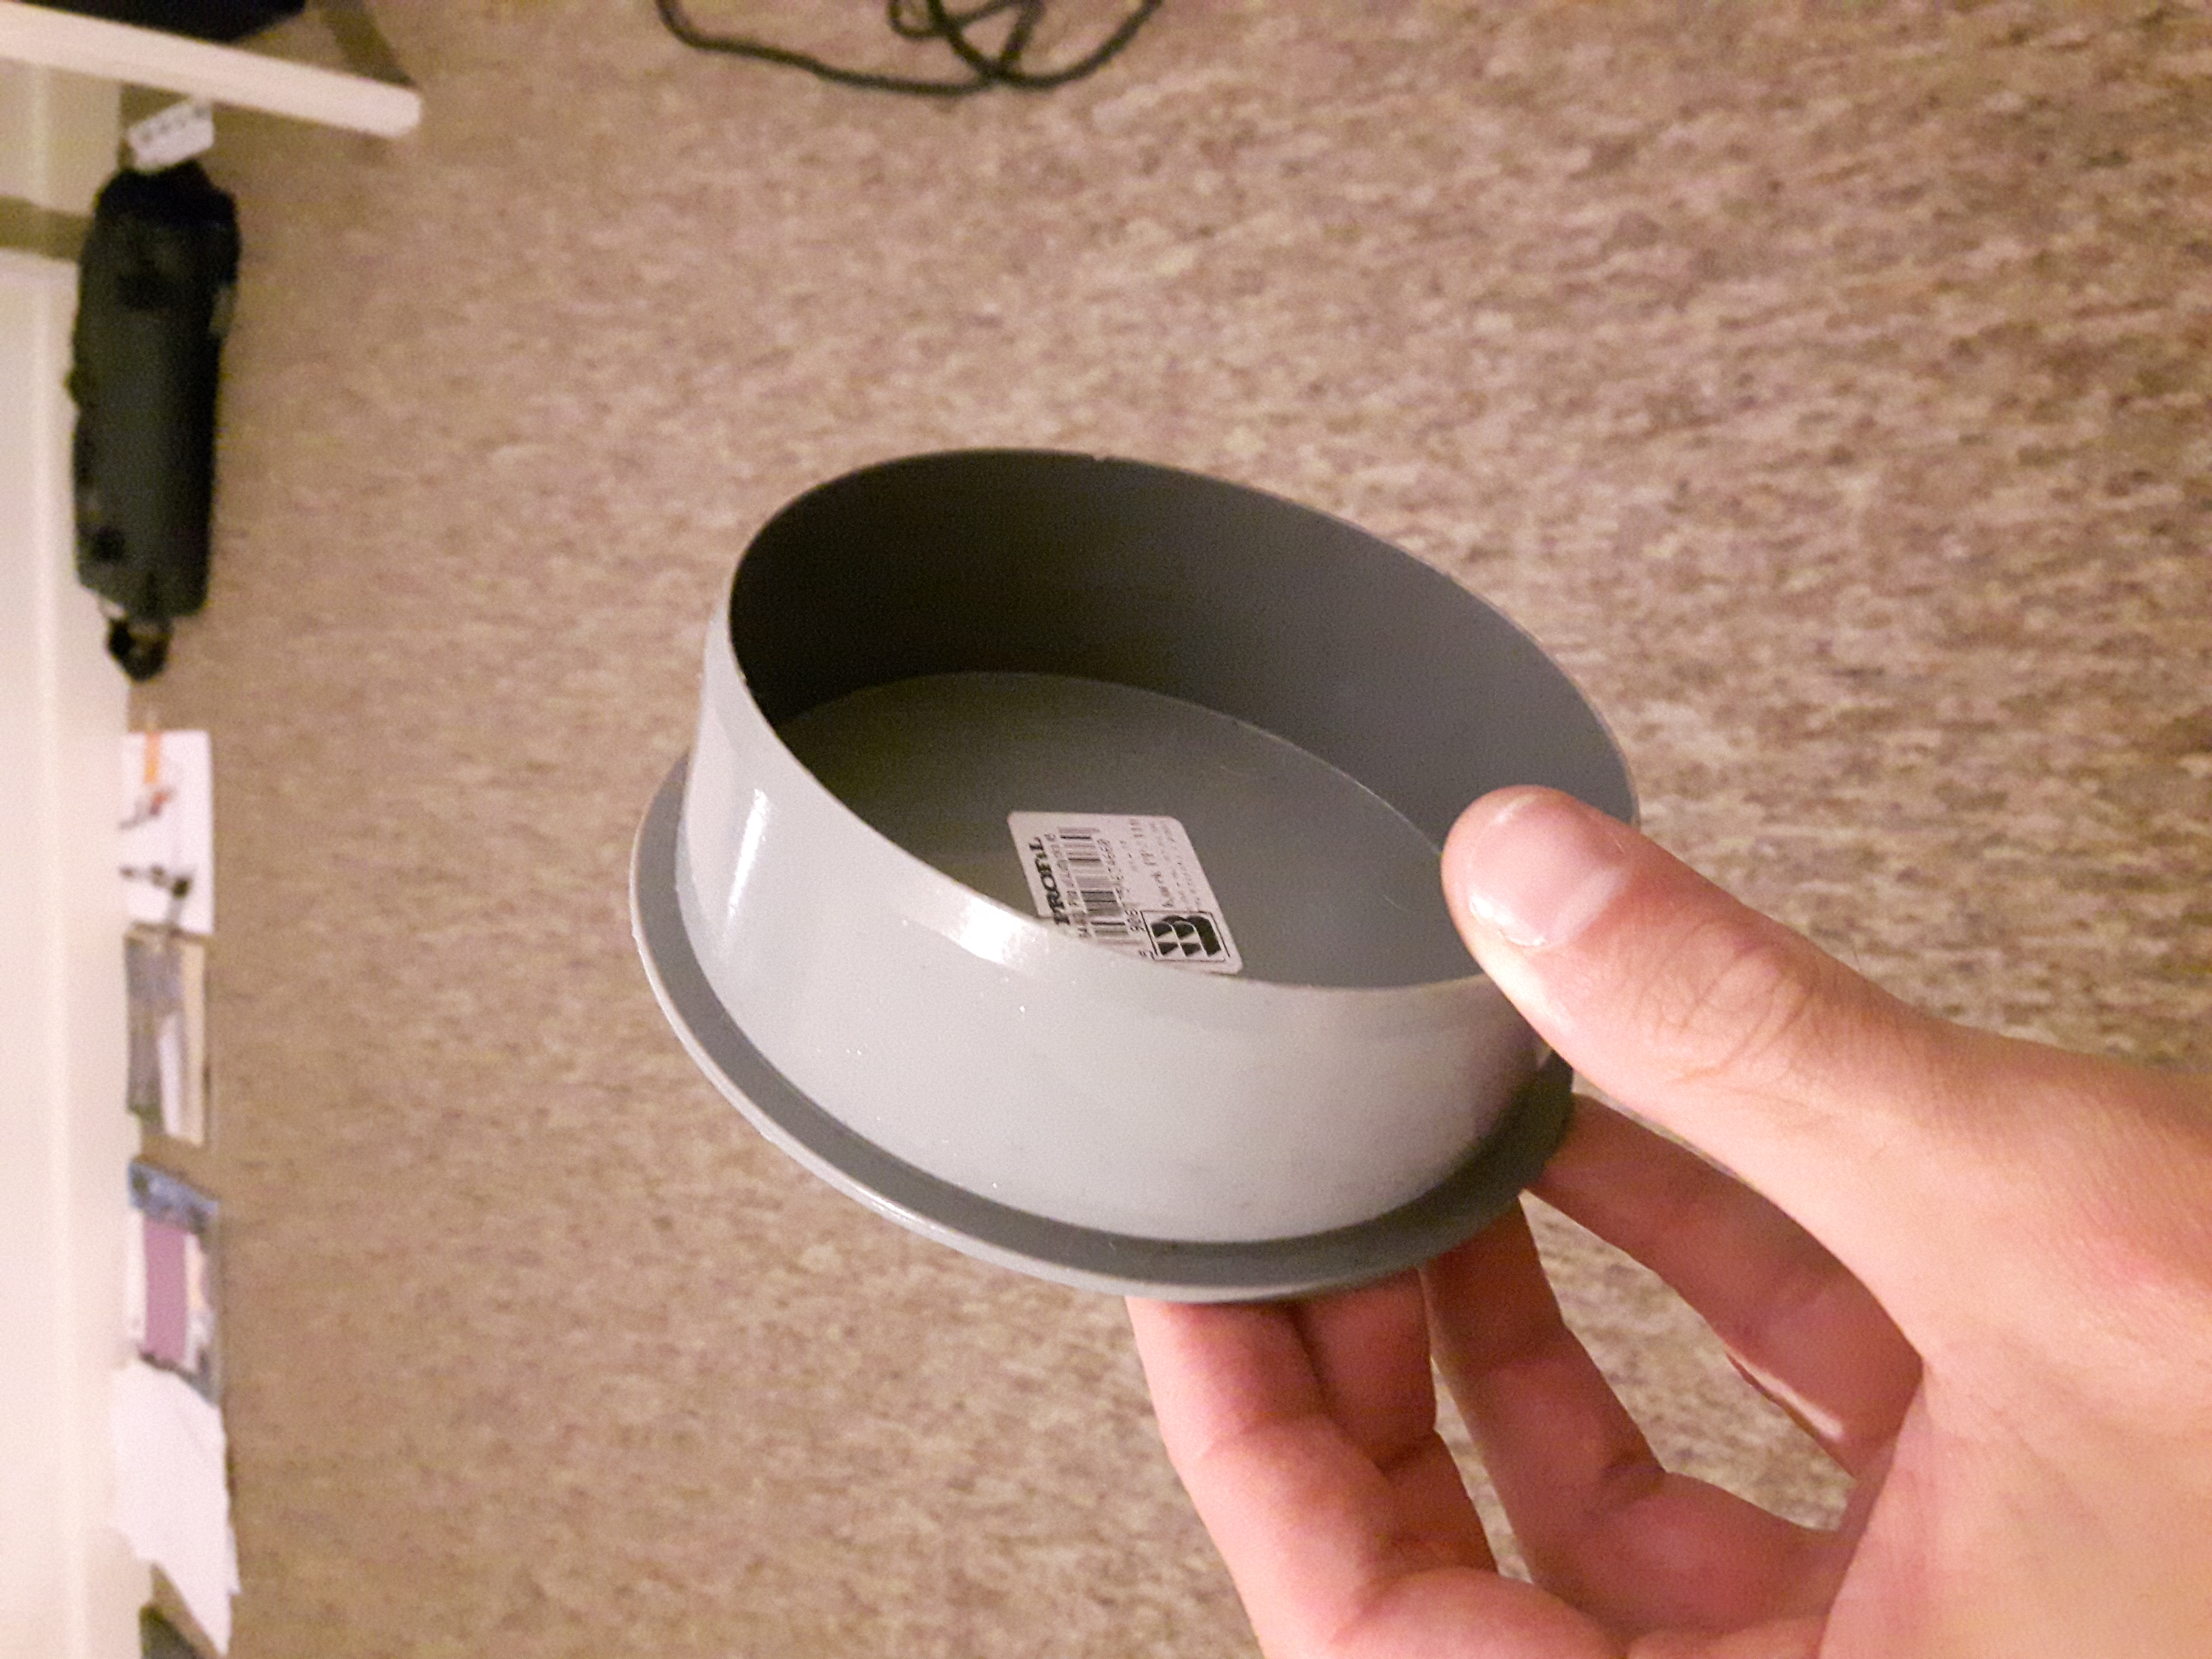
\includegraphics[width=\linewidth,angle=270]{20160826_213233.jpg}
\end{minipage}
\caption{Socket plug used to manufacture the aft and forward plug.}
\label{fig:socketPlug}
\end{figure}

%-------------------------------------------------------------------------------
\subsection{Ardunio pinout}\label{ssection:arduinoPinout}

Table \ref{tab:pinoutMain} describes all of the Arduino connections used by the ROV. Thrust direction pins are responsible for switching the relays on the motor control board via mosfet transistors, and throttle pins are connected to the ESCs directly and control motor rpm using PWM signals (see section~\ref{ssection:motorControlBoard} for details).

\begin{table}[h]
\centering
\caption{Pinout showing Arduino connections.}
\label{tab:pinoutMain}
\begin{tabular}{@{}ll@{}}
\toprule
\textbf{Pin  no.} & \textbf{Connect net} \\ \midrule
2 & Motor port horizontal - thrust direction \\
3 & Motor port horizontal - throttle \\
4 & Motor starboard horizontal - thrust direction \\
5 & Motor starboard horizontal - throttle \\
6 & Motor port vertical - throttle \\
7 & Motor port vertical - thrust direction \\
8 & Motor starboard vertical - thrust direction \\
9 & Motor starboard vertical - throttle \\
12 & Forward LED on/off \\
A0 & Pressure transducer analogue input \\
5 V & Pressure transducer VDD \\
\bottomrule
\end{tabular}
\end{table}

%===============================================================================
\section{Pressure vessel}\label{section:pressureVessel}

%-------------------------------------------------------------------------------
\subsection{Aft plug}\label{sscetion:aftPlug}
The aft plug is made of a~PVC socket plug shown in Fig.~\ref{fig:socketPlug}. Two holes were punched in it - one, into which the pressure transducer is screwed in, as described in section~\ref{ssection:pressureSensor}, and one, which houses the umbilical connector described in section~\ref{ssection:connectorOnTheROV}.

The external side of the aft plug (the wet side of the ROV), with the pressure transducer and umbilical connector mounted, is shown in Fig.~\ref{fig:externalSideOfTheAftPlug}. Its internal side is shown in Fig.~\ref{fig:internalSideOfTheAftPlug}; the body of the pressure sensor, CAT5 cable, power chord, and 12 motor wires (three signals per each of the four motors) can be seen on this side. The plug can be removed from the main pressure vessel to enable inspection and modification of the interior of the ROV. In order to ease the process and improve the water-tightness, silicone lubricant from Fig.~\ref{fig:lubricant} is applied on the aft plug before it is slid into the main pressure vessel. Once in place, the aft plug is secured using a~water-resistant duct tape.

\begin{figure}[htb]
\begin{minipage}[b]{1\linewidth}
  \centering
	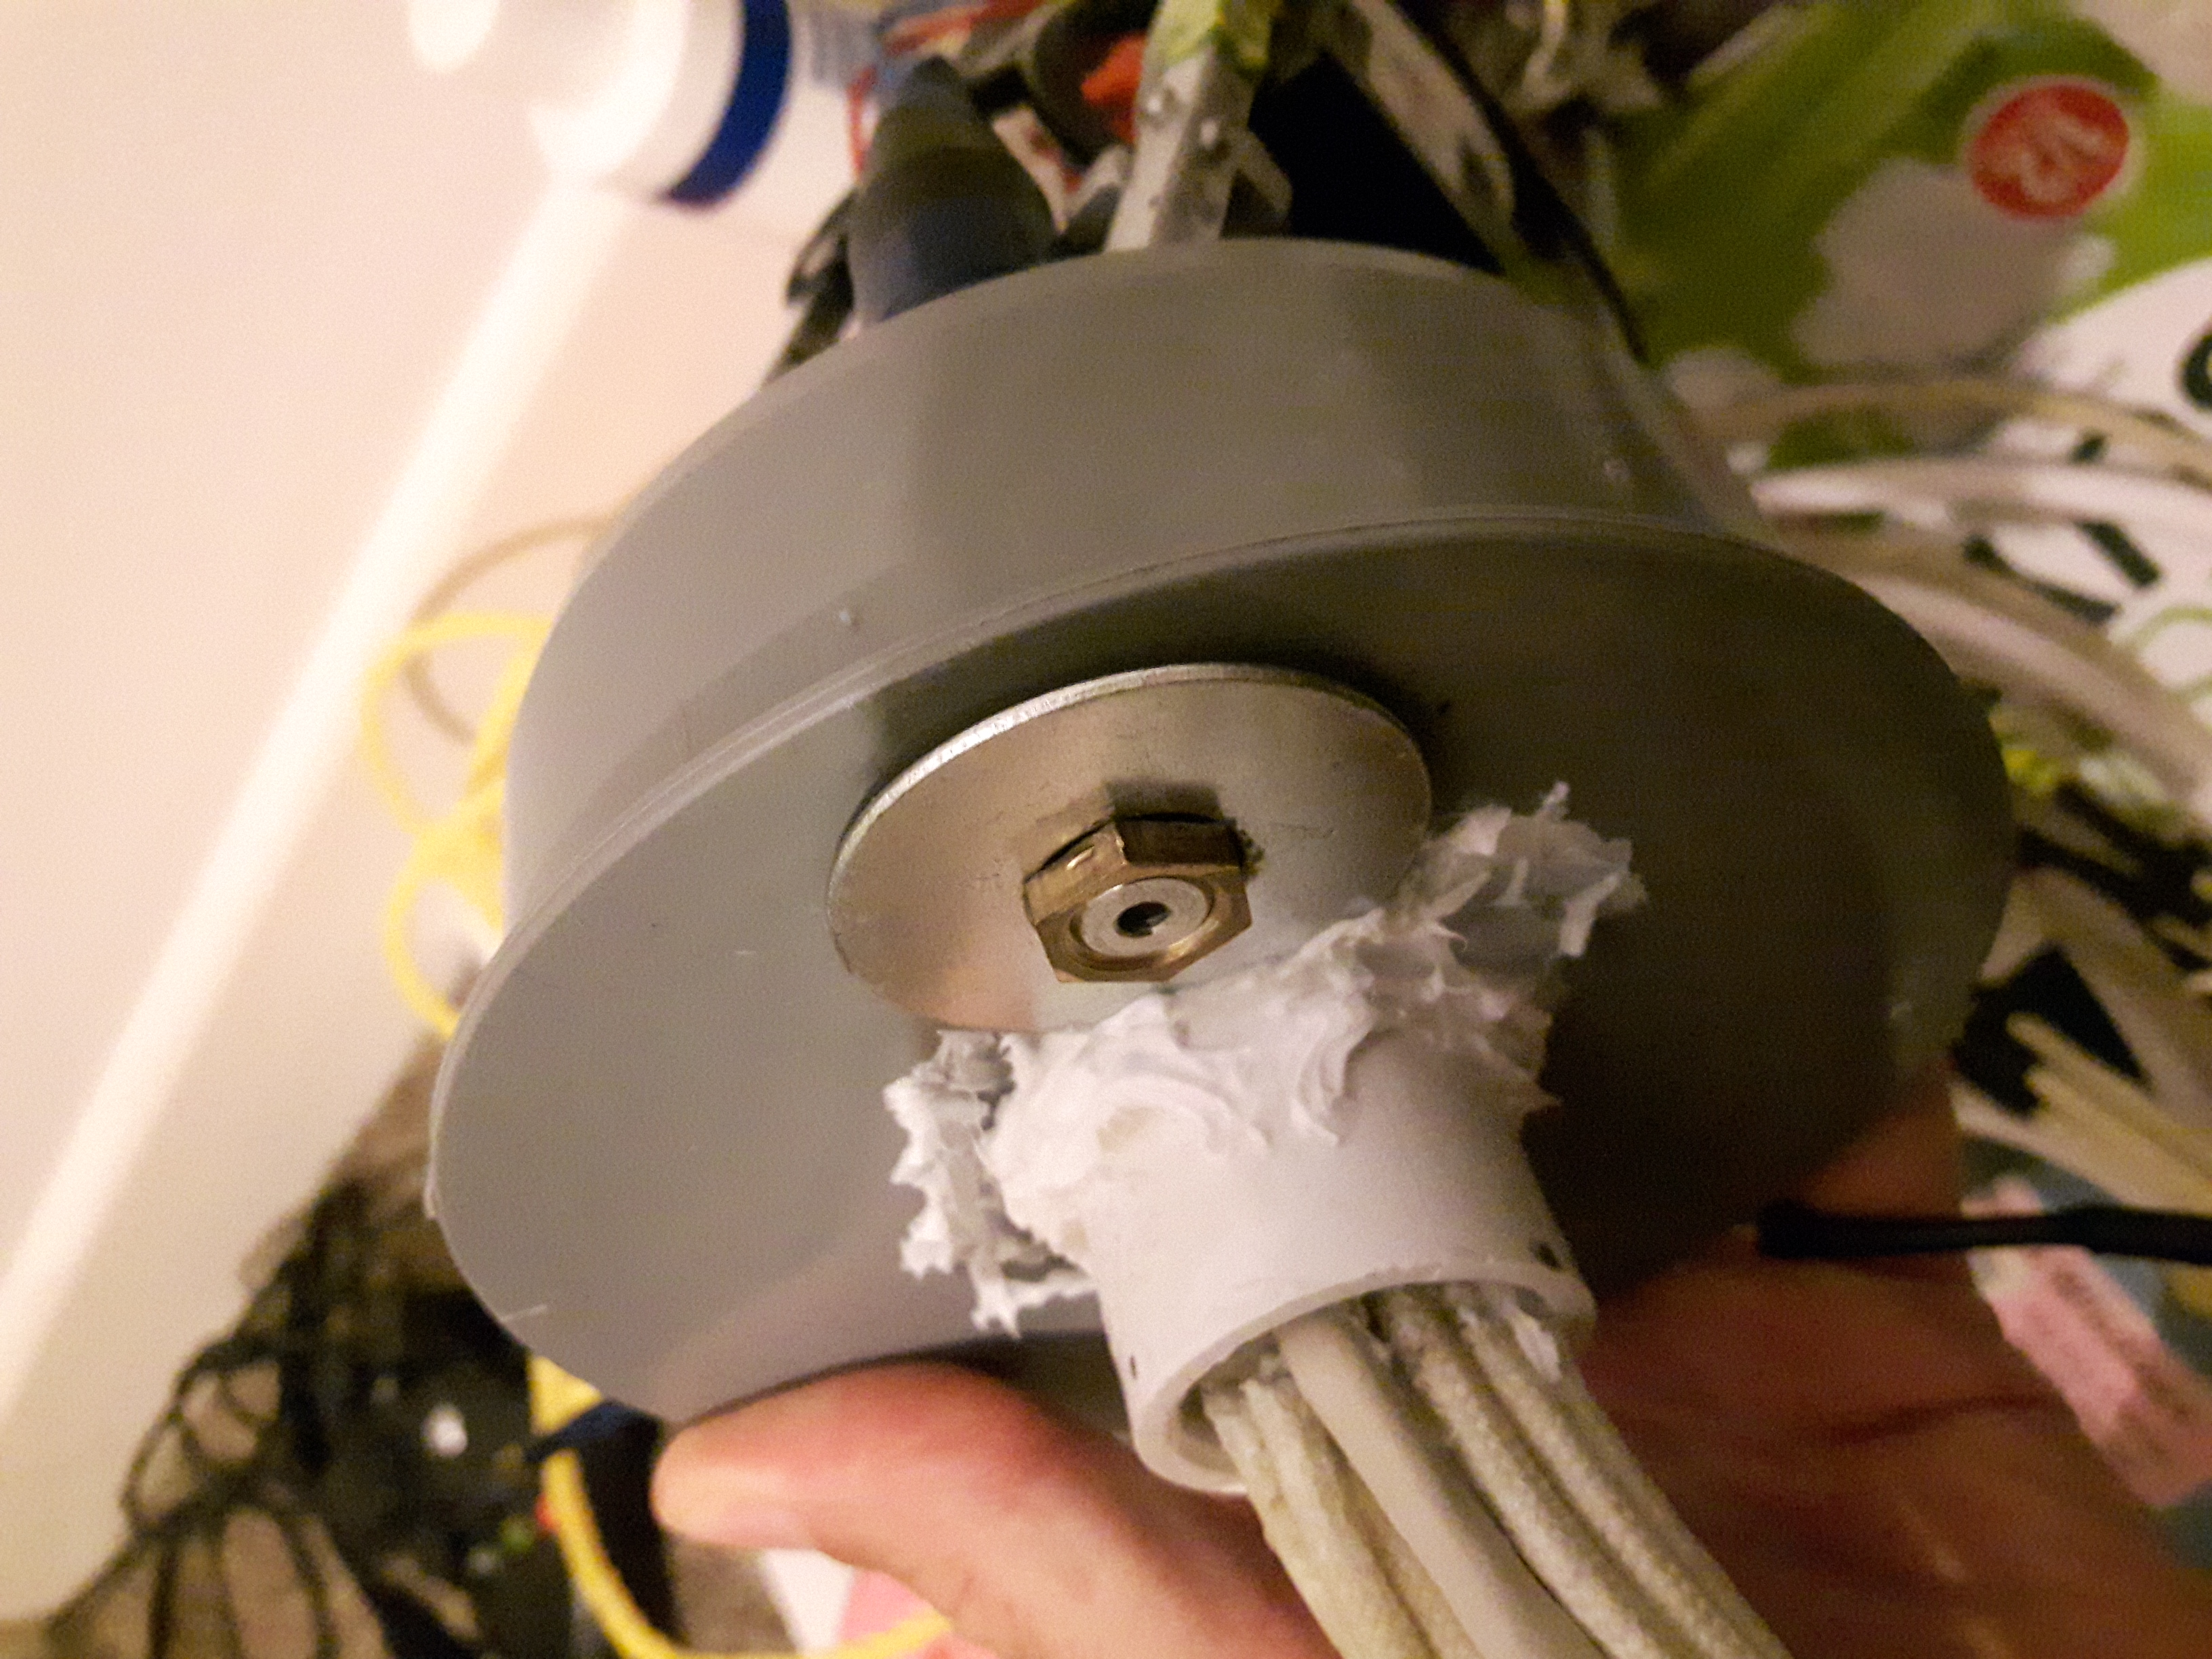
\includegraphics[width=\linewidth,angle=270]{20160827_212715.jpg}
\end{minipage}
\caption{External side of the aft plug with the pressure sensor and umbilical connector mounted.}
\label{fig:externalSideOfTheAftPlug}
\end{figure}

\begin{figure}[htb]
\begin{minipage}[b]{1\linewidth}
  \centering
	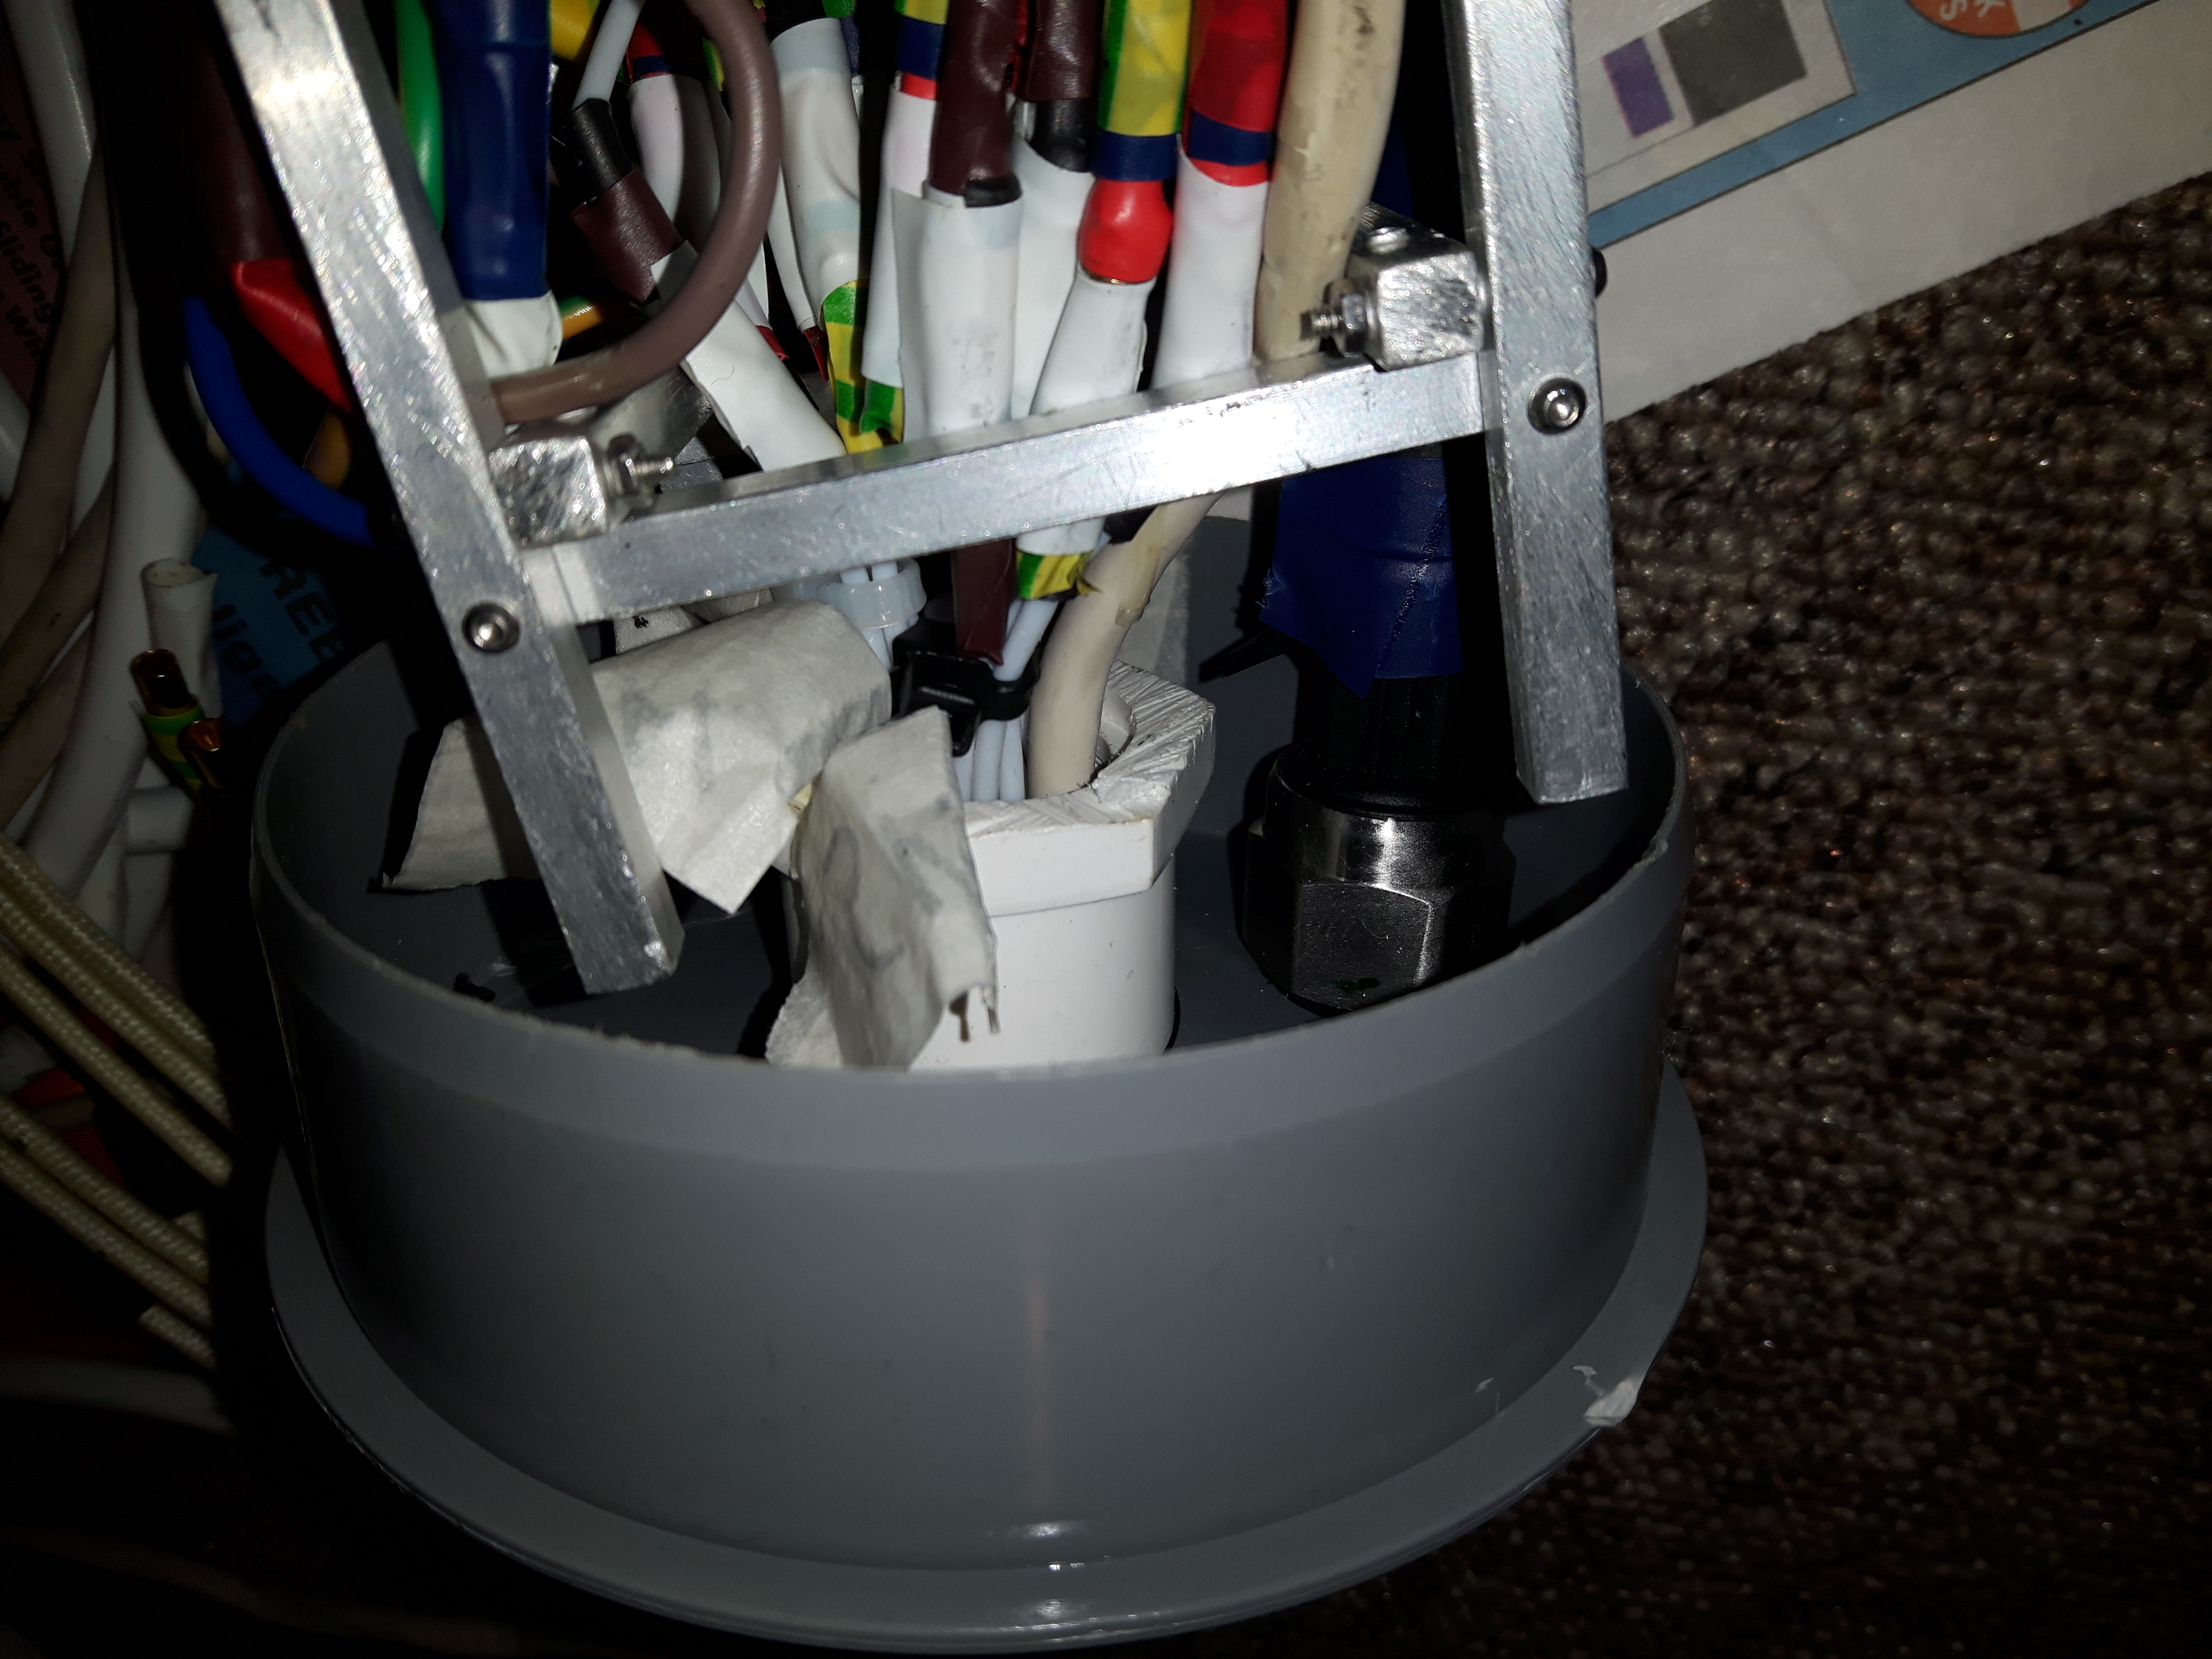
\includegraphics[width=\linewidth,angle=180]{20160827_213602.jpg}
\end{minipage}
\caption{Internal side of the aft plug with the pressure sensor and umbilical connectors mounted. The CAT5 cable is plugged into the USB range extender, and all motor wires are connected to the ESCs and the motor control board.}
\label{fig:internalSideOfTheAftPlug}
\end{figure}

\begin{figure}[htb]
\begin{minipage}[b]{1\linewidth}
  \centering
	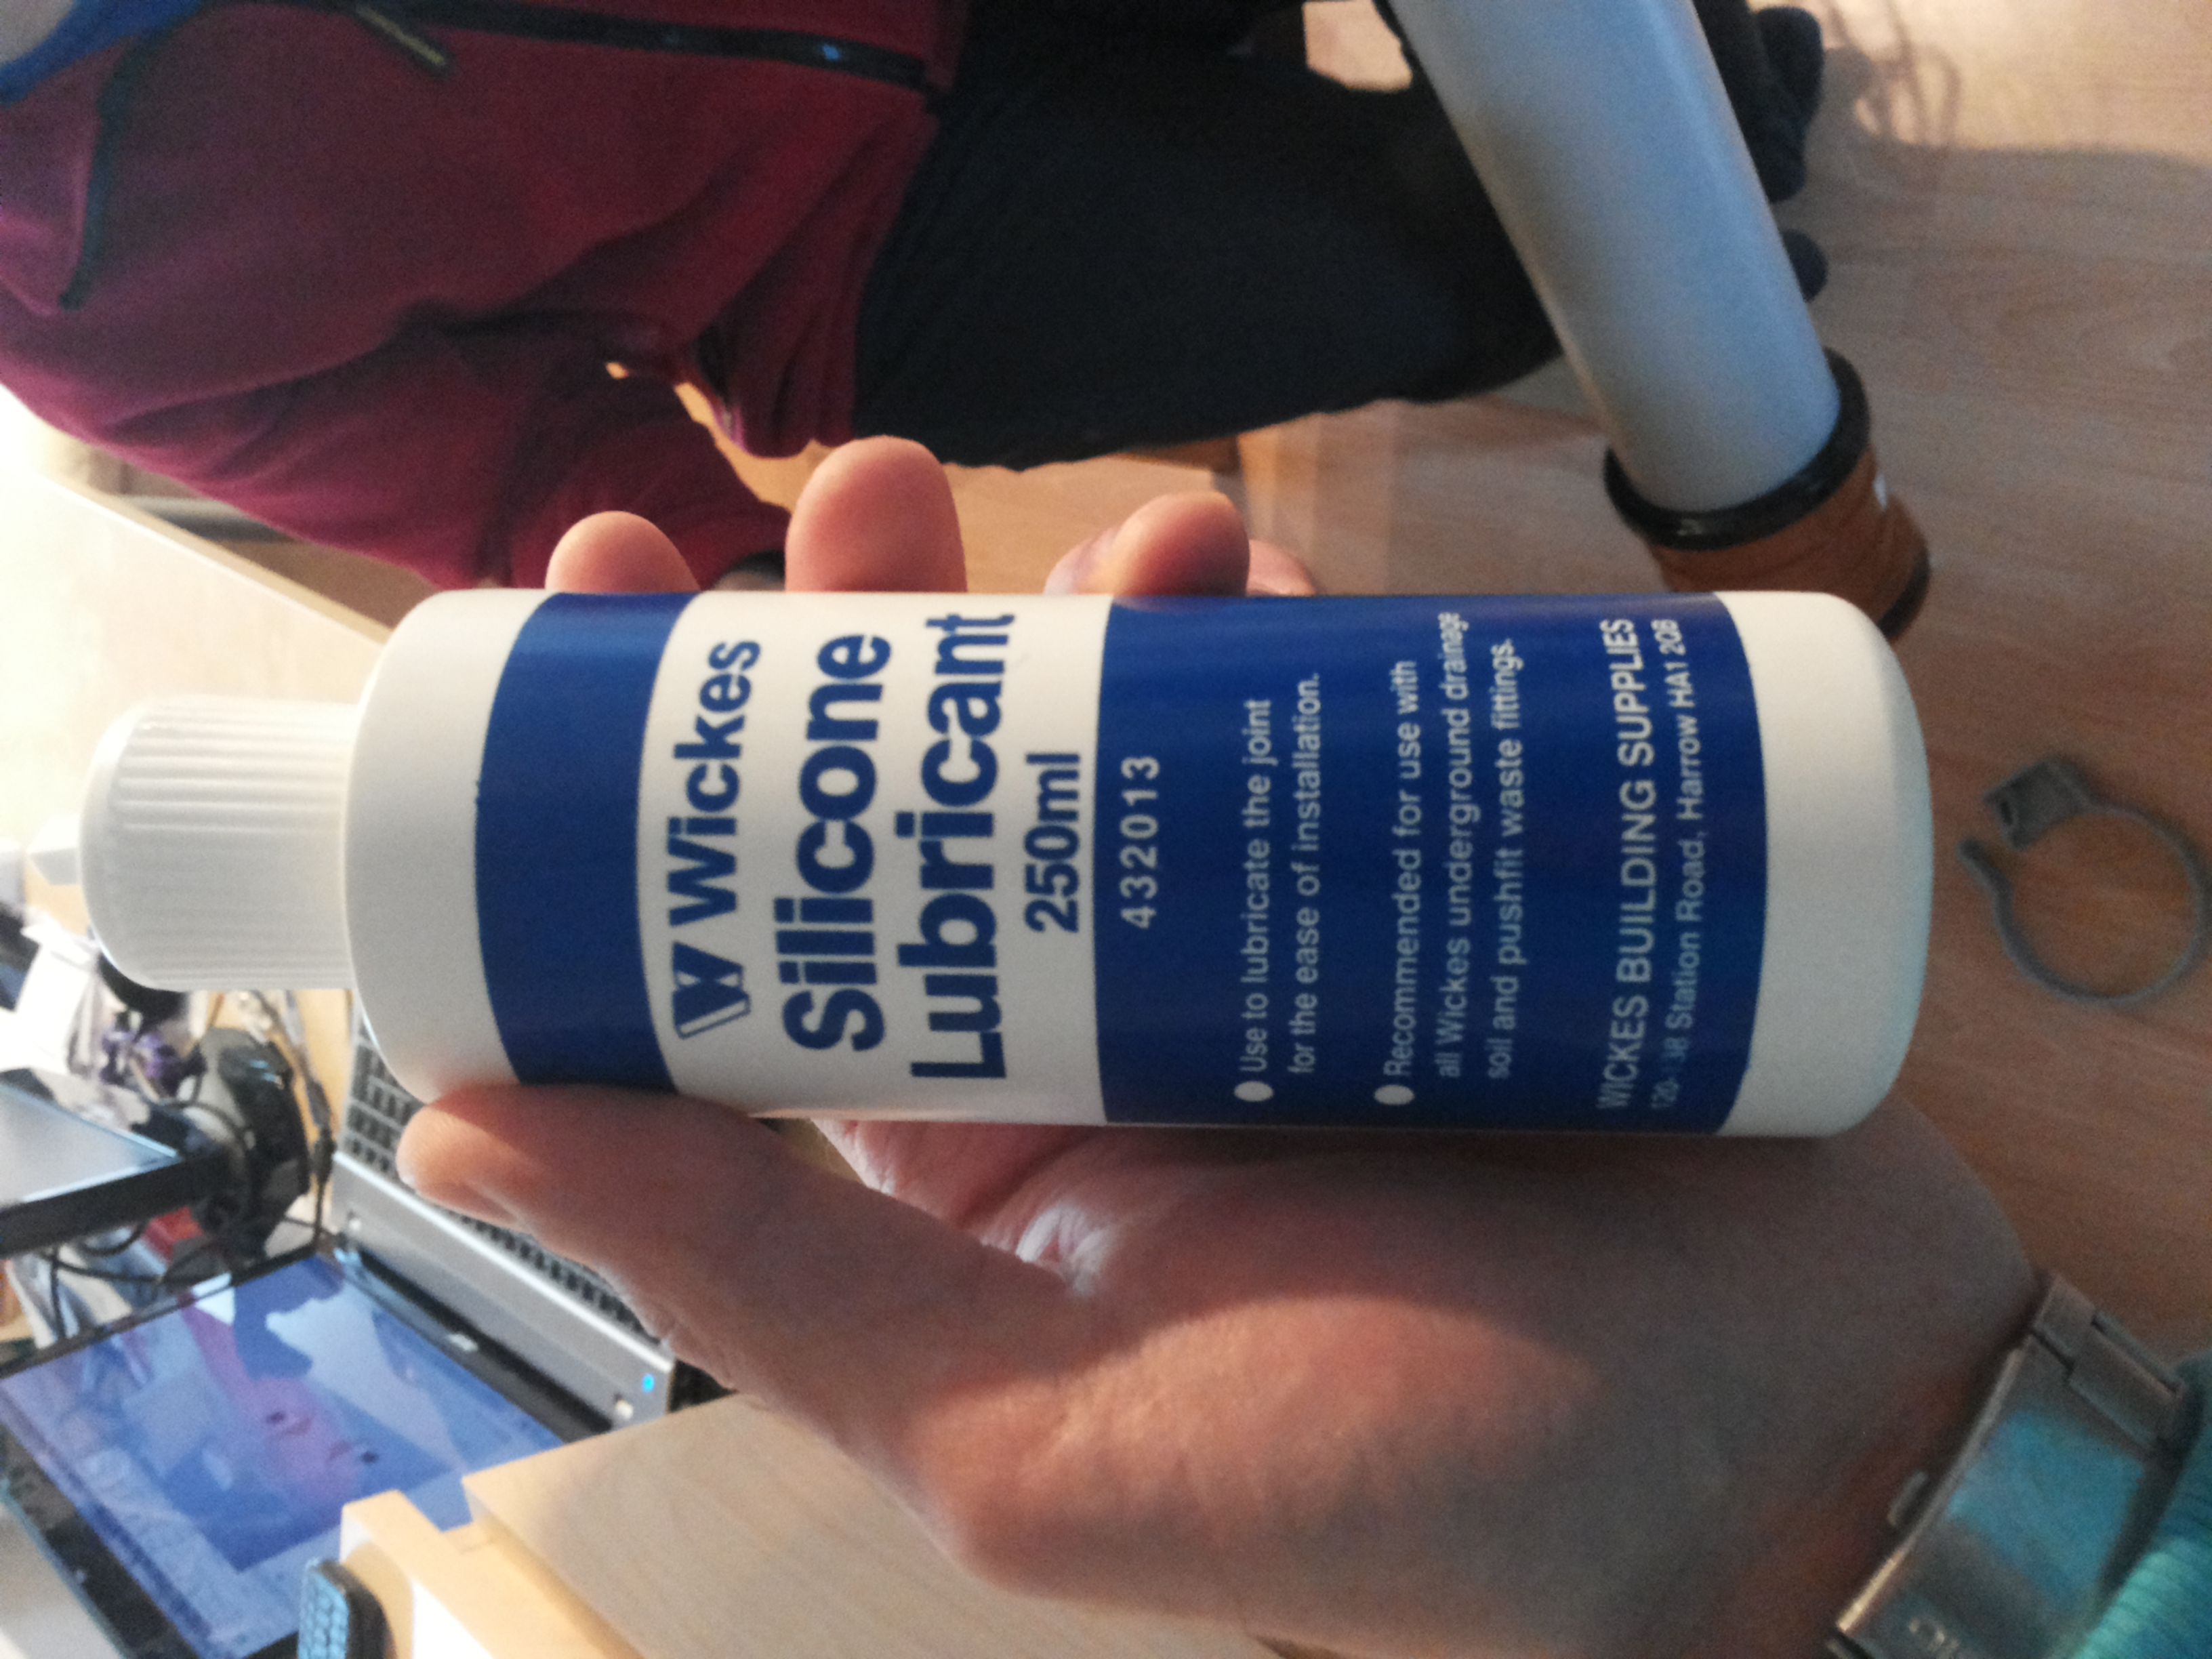
\includegraphics[width=\linewidth,angle=270]{20151122_144346.jpg}
\end{minipage}
\caption{When the aft plug is slid into the main pressure vessel, this silicone lubricant is applied onto it to ease the assembly and improve the seal.}
\label{fig:lubricant}
\end{figure}

%-------------------------------------------------------------------------------
\subsection{Forward plug}\label{ssection:forwardPlug}
The forward plug was manufactured from a~socket plug identical to the one used for manufacture of the aft plug (shown in Fig.~\ref{fig:socketPlug}). The forward plug has to enable the camera to photograph the space in front of the ROV to enable remote operation. To this end, a~hole was cut in the socket plug as shown in Fig.~\ref{fig:cuttingAHole}. A~window was cut out of a~\unit[4]{mm} thick plexiglass, which was glued onto the outer side of the socket plug using a~two-part epoxy glue. The complete forward plug is fixed in the pressure vessel using silicone; this provides both structural strength and makes the connection water-tight. The complete forward plug, mounted into the pressure vessel, can be seen in Fig.~\ref{fig:assembledPressureVessel}.

\begin{figure}[htb]
\begin{minipage}[b]{1\linewidth}
  \centering
	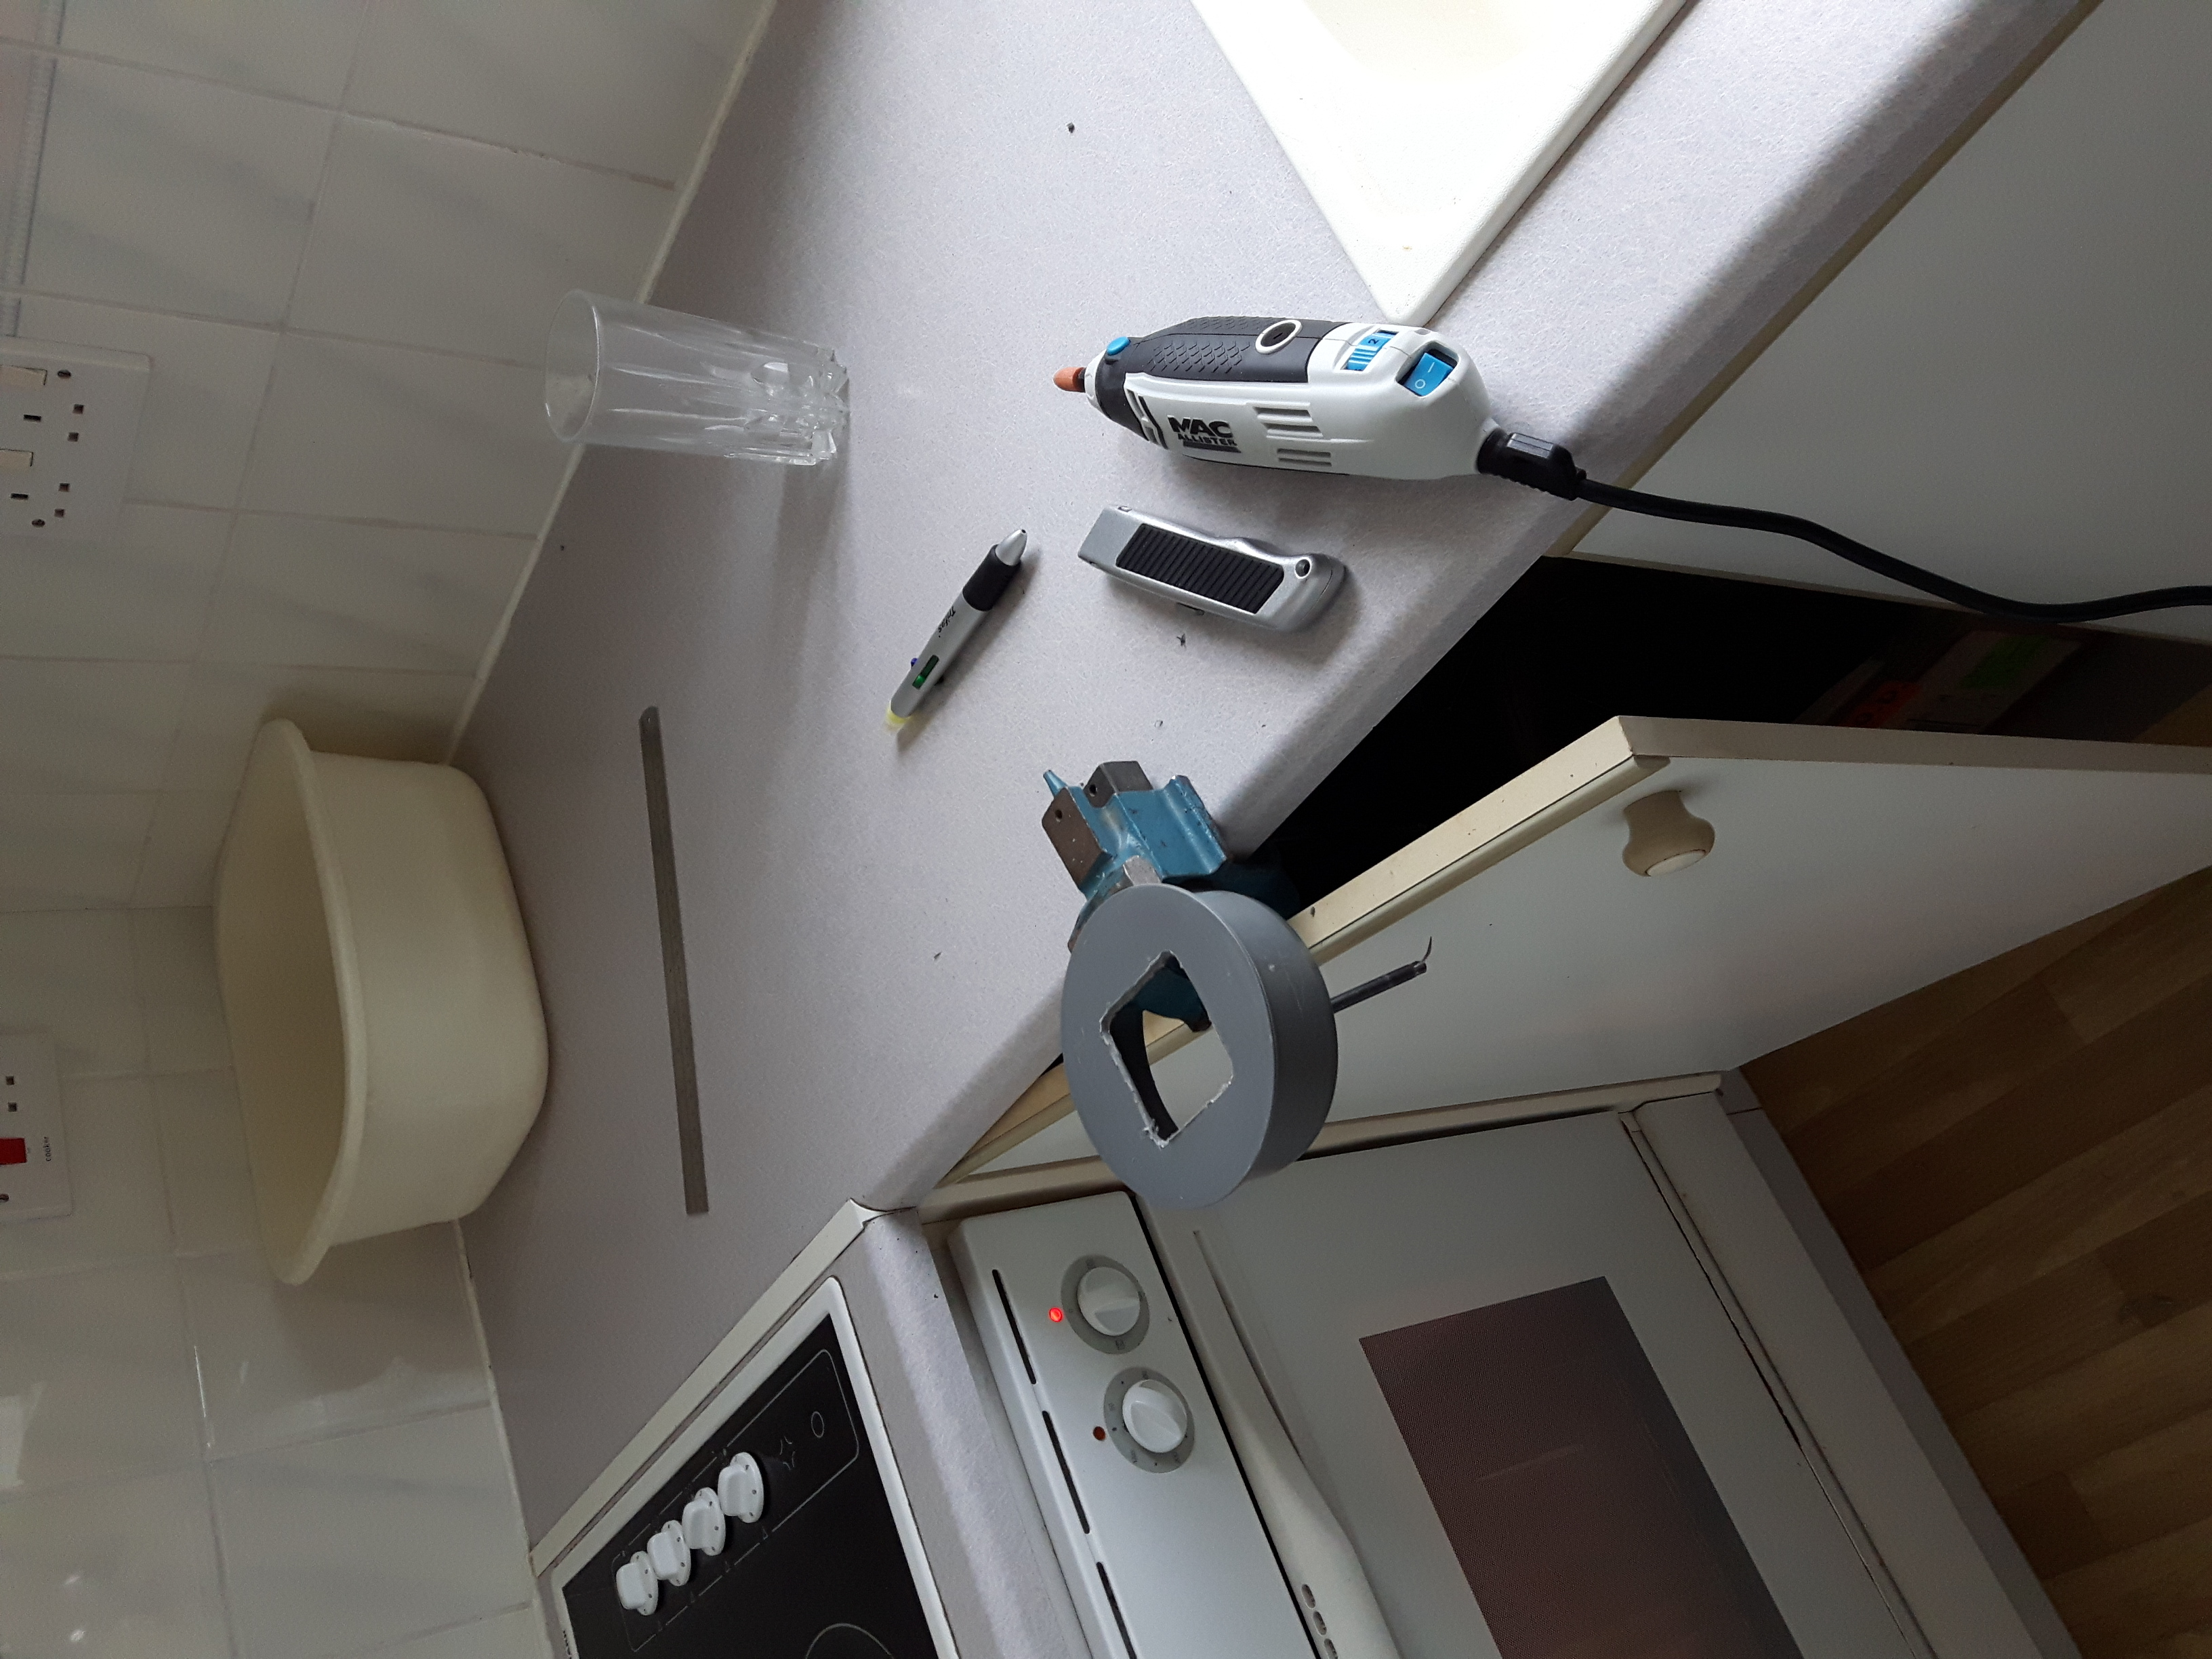
\includegraphics[width=\linewidth,angle=270]{20160418_183948.jpg}
\end{minipage}
\caption{Cutting a~hole in the socket plug to provide a~viewing window for the camera.}
\label{fig:cuttingAHole}
\end{figure}

%-------------------------------------------------------------------------------
\subsection{Main vessel}
The main pressure vessel is made of two PVC pipes, shown in Fig.~\ref{fig:pressureVesselPipes}. The orange double-sided socket is located on the bow of the ROV. The grey socket pipe was cut to the right length (to provide sufficient displacement), slid into the orange double socket, and secured using silicone. This connection is water-tight, and provides structural rigidity and strength. The assembled pressure vessel is shown in Fig.~\ref{fig:assembledPressureVessel}.

Apparently, PVC pipes of the same dimensions can have different masses, depending on their manufacturer. The ones used for this ROV were bought at Wickes, a~UK DIY supermarket.

\begin{figure}[htb]
\begin{minipage}[b]{1\linewidth}
  \centering
	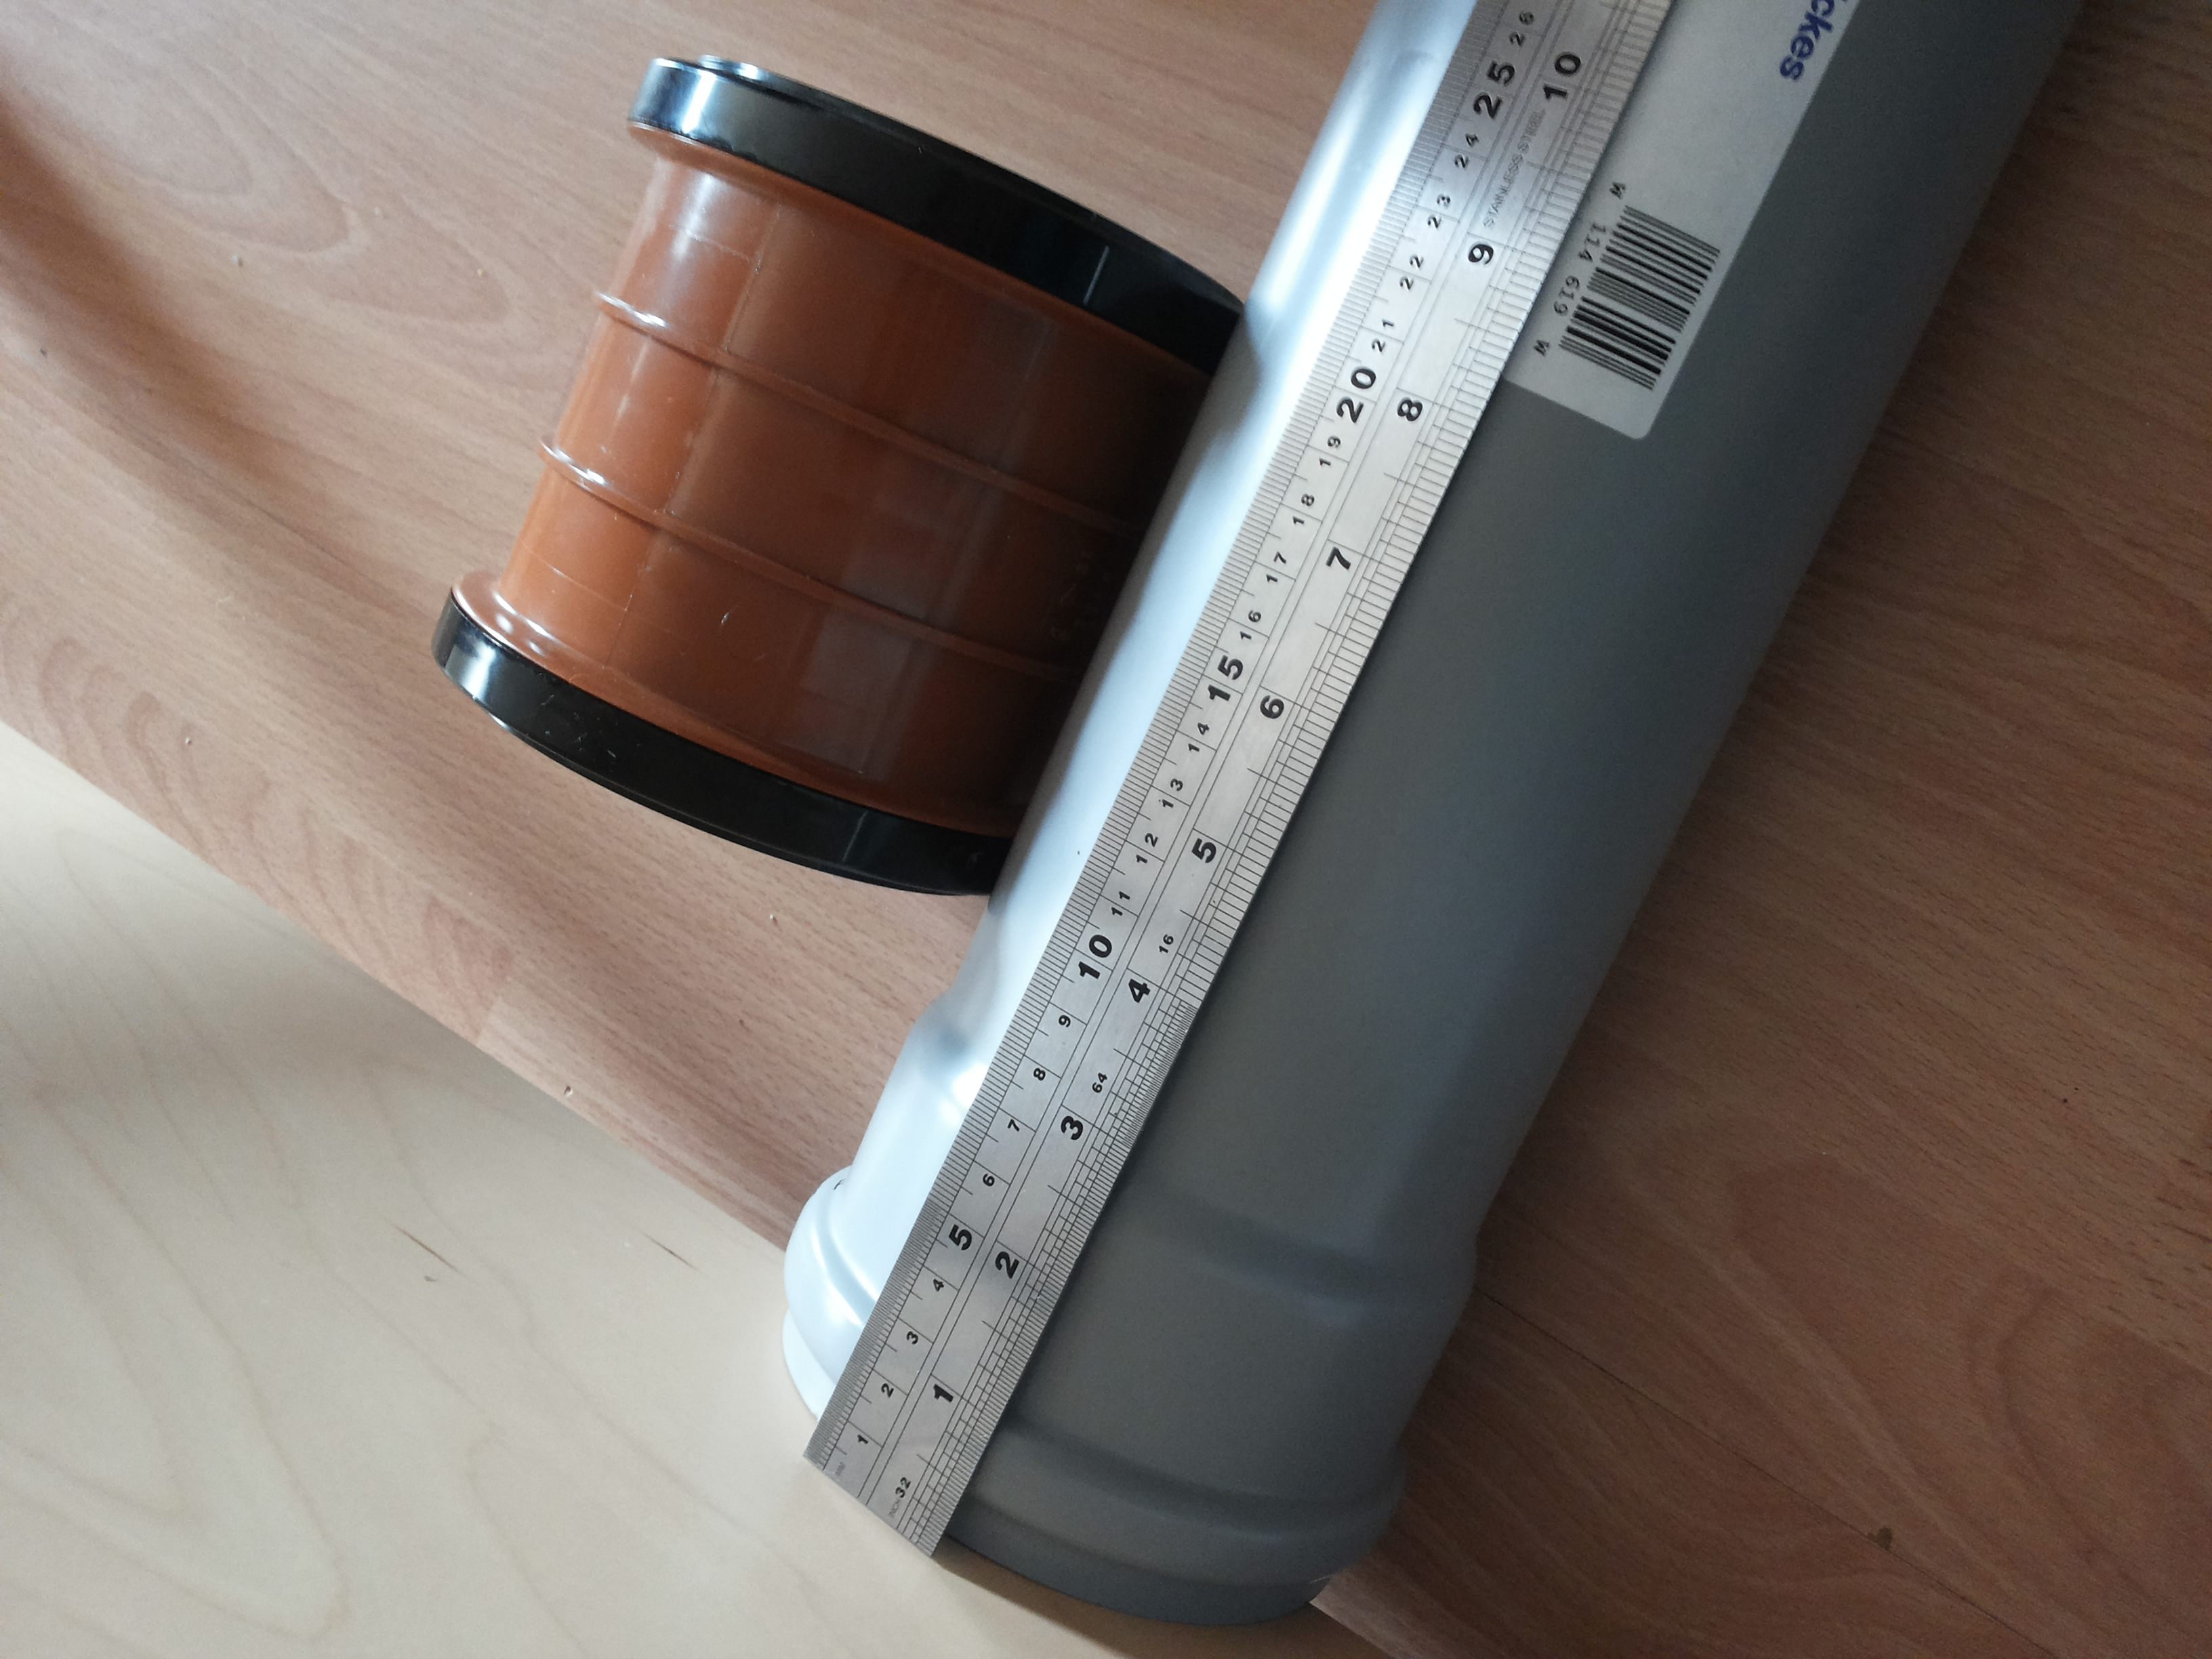
\includegraphics[width=\linewidth]{20151122_142423.jpg}
\end{minipage}
\caption{The pressure vessel consists of two main parts - an orange double-sided socket and a~grey socket pipe.}
\label{fig:pressureVesselPipes}
\end{figure}

\begin{figure}[htb]
\begin{minipage}[b]{1\linewidth}
  \centering
	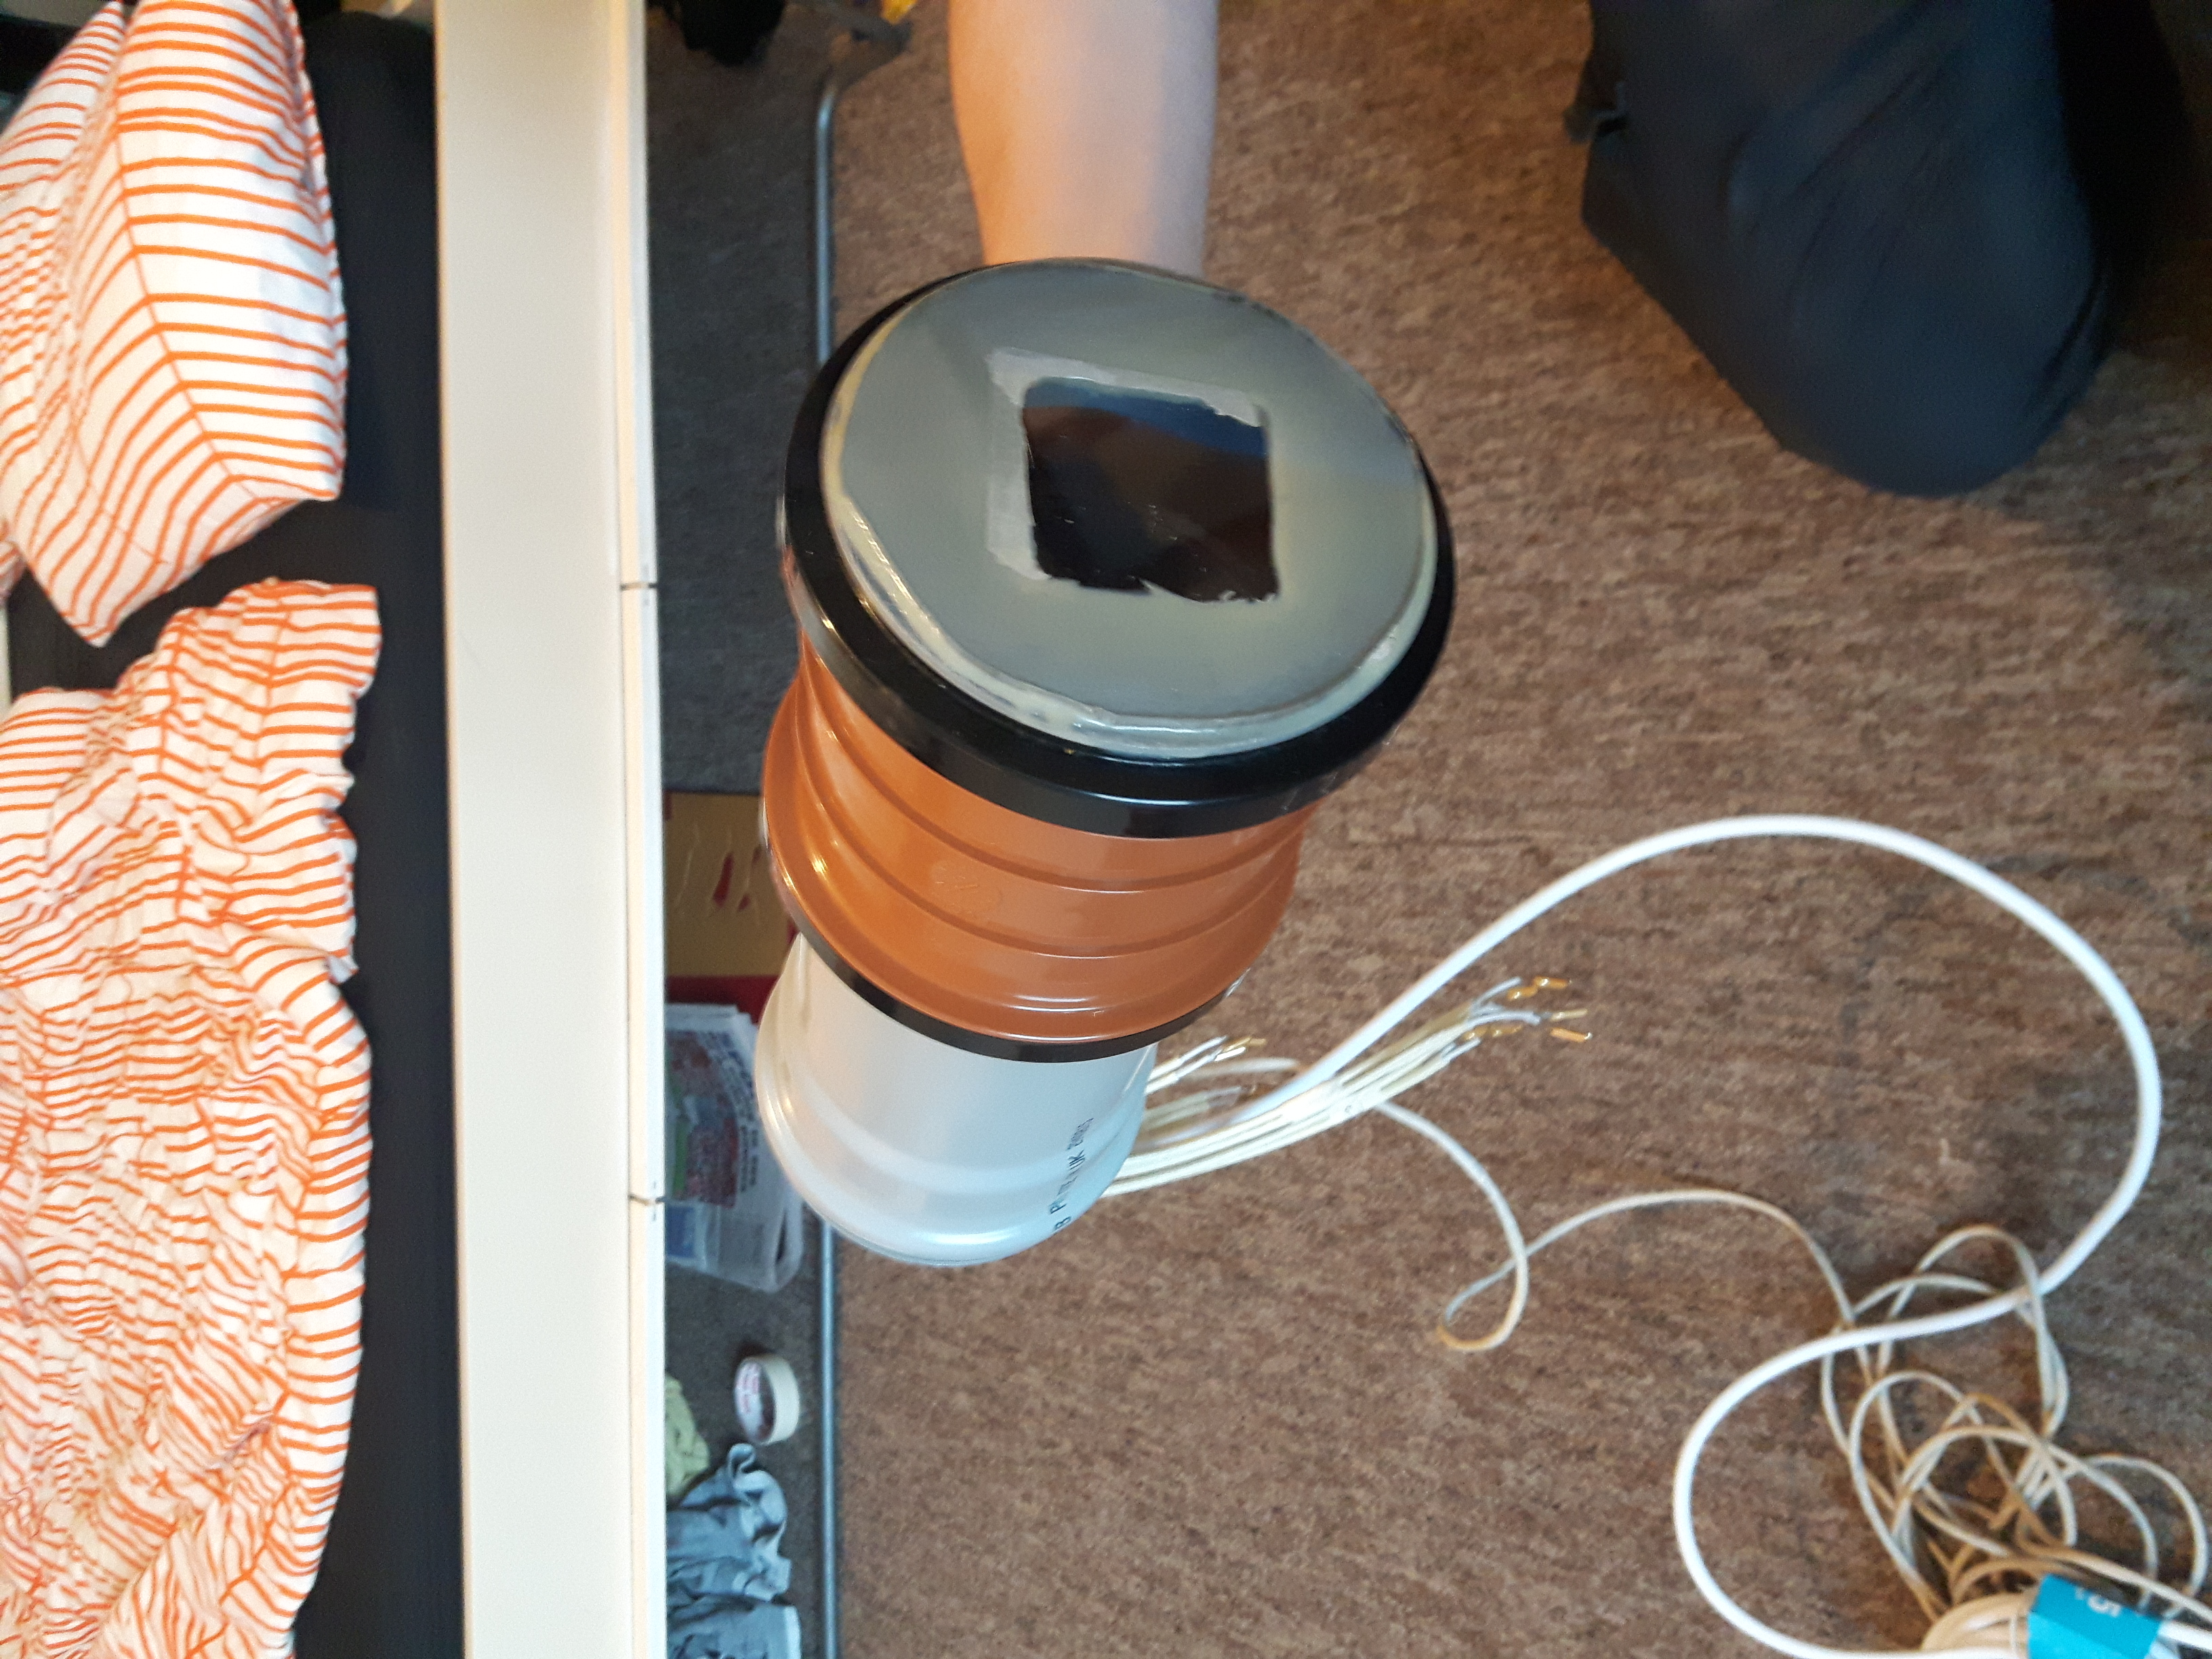
\includegraphics[width=\linewidth,angle=270]{20160507_195201.jpg}
\end{minipage}
\caption{Assembled pressure vessel.}
\label{fig:assembledPressureVessel}
\end{figure}

\clearpage % Avoid "too many unprocessed floats" error.

%===============================================================================
\section{External structure}\label{section:externalStructure}
For the naming convention and location of the components of the external structure, please refer to Fig.~\ref{fig:rovGAsExternal}.

%-------------------------------------------------------------------------------
\subsection{Transversals and longitudinals}
Side longitudinals, trasnverse clip stiffeners, and landing sleds were made of \unit[2]{mm} thick, \unit[20]{mm} wide rolled steel. In order to reduce their mass, M10 holes were drilled along their lengths. The structure is bolted together using M3 bolts. All the metal parts are painted to reduce corrosion.

%-------------------------------------------------------------------------------
\subsection{Pressure vessel mounting}
In order to mate the external metal structure with the pressure vessel made of PVC pipes, PVC socket brackets are used. The landing sleds and transversal clip stiffeners are bolted onto the default mounting holes in the brackets, which can be seen on the bottom of Fig.~\ref{fig:motorMountingDetails:label:a}. In order to mount the side longitudinals and motors, additional M3 holes were drilled in the socket brackets, as shown in Fig.~\ref{fig:brackets} and Fig.~\ref{fig:motorMountingDetails:label:a}.

The steel structure was bolted together and onto the socket brackets, but one side of every bracket was left free (one bolt going through the landing sled and transverse clip stiffener was not inserted). Then, the pressure vessel was inserted into the brackets, and the loose end of every bracket was fixed in place around the pressure vessel by bolting it onto the sled and the transverse clip stiffener.

To prevent the steel structure from slipping along the pressure vessel, the bow bracket was placed in the groove in the double socket pipe, as shown in Fig.~\ref{fig:brackets}. To stop the brackets from rotating around the pressure vessel, both of them were glued to it using a~two-part epoxy glue.

\begin{figure}[htb]
\begin{minipage}[b]{1\linewidth}
  \centering
	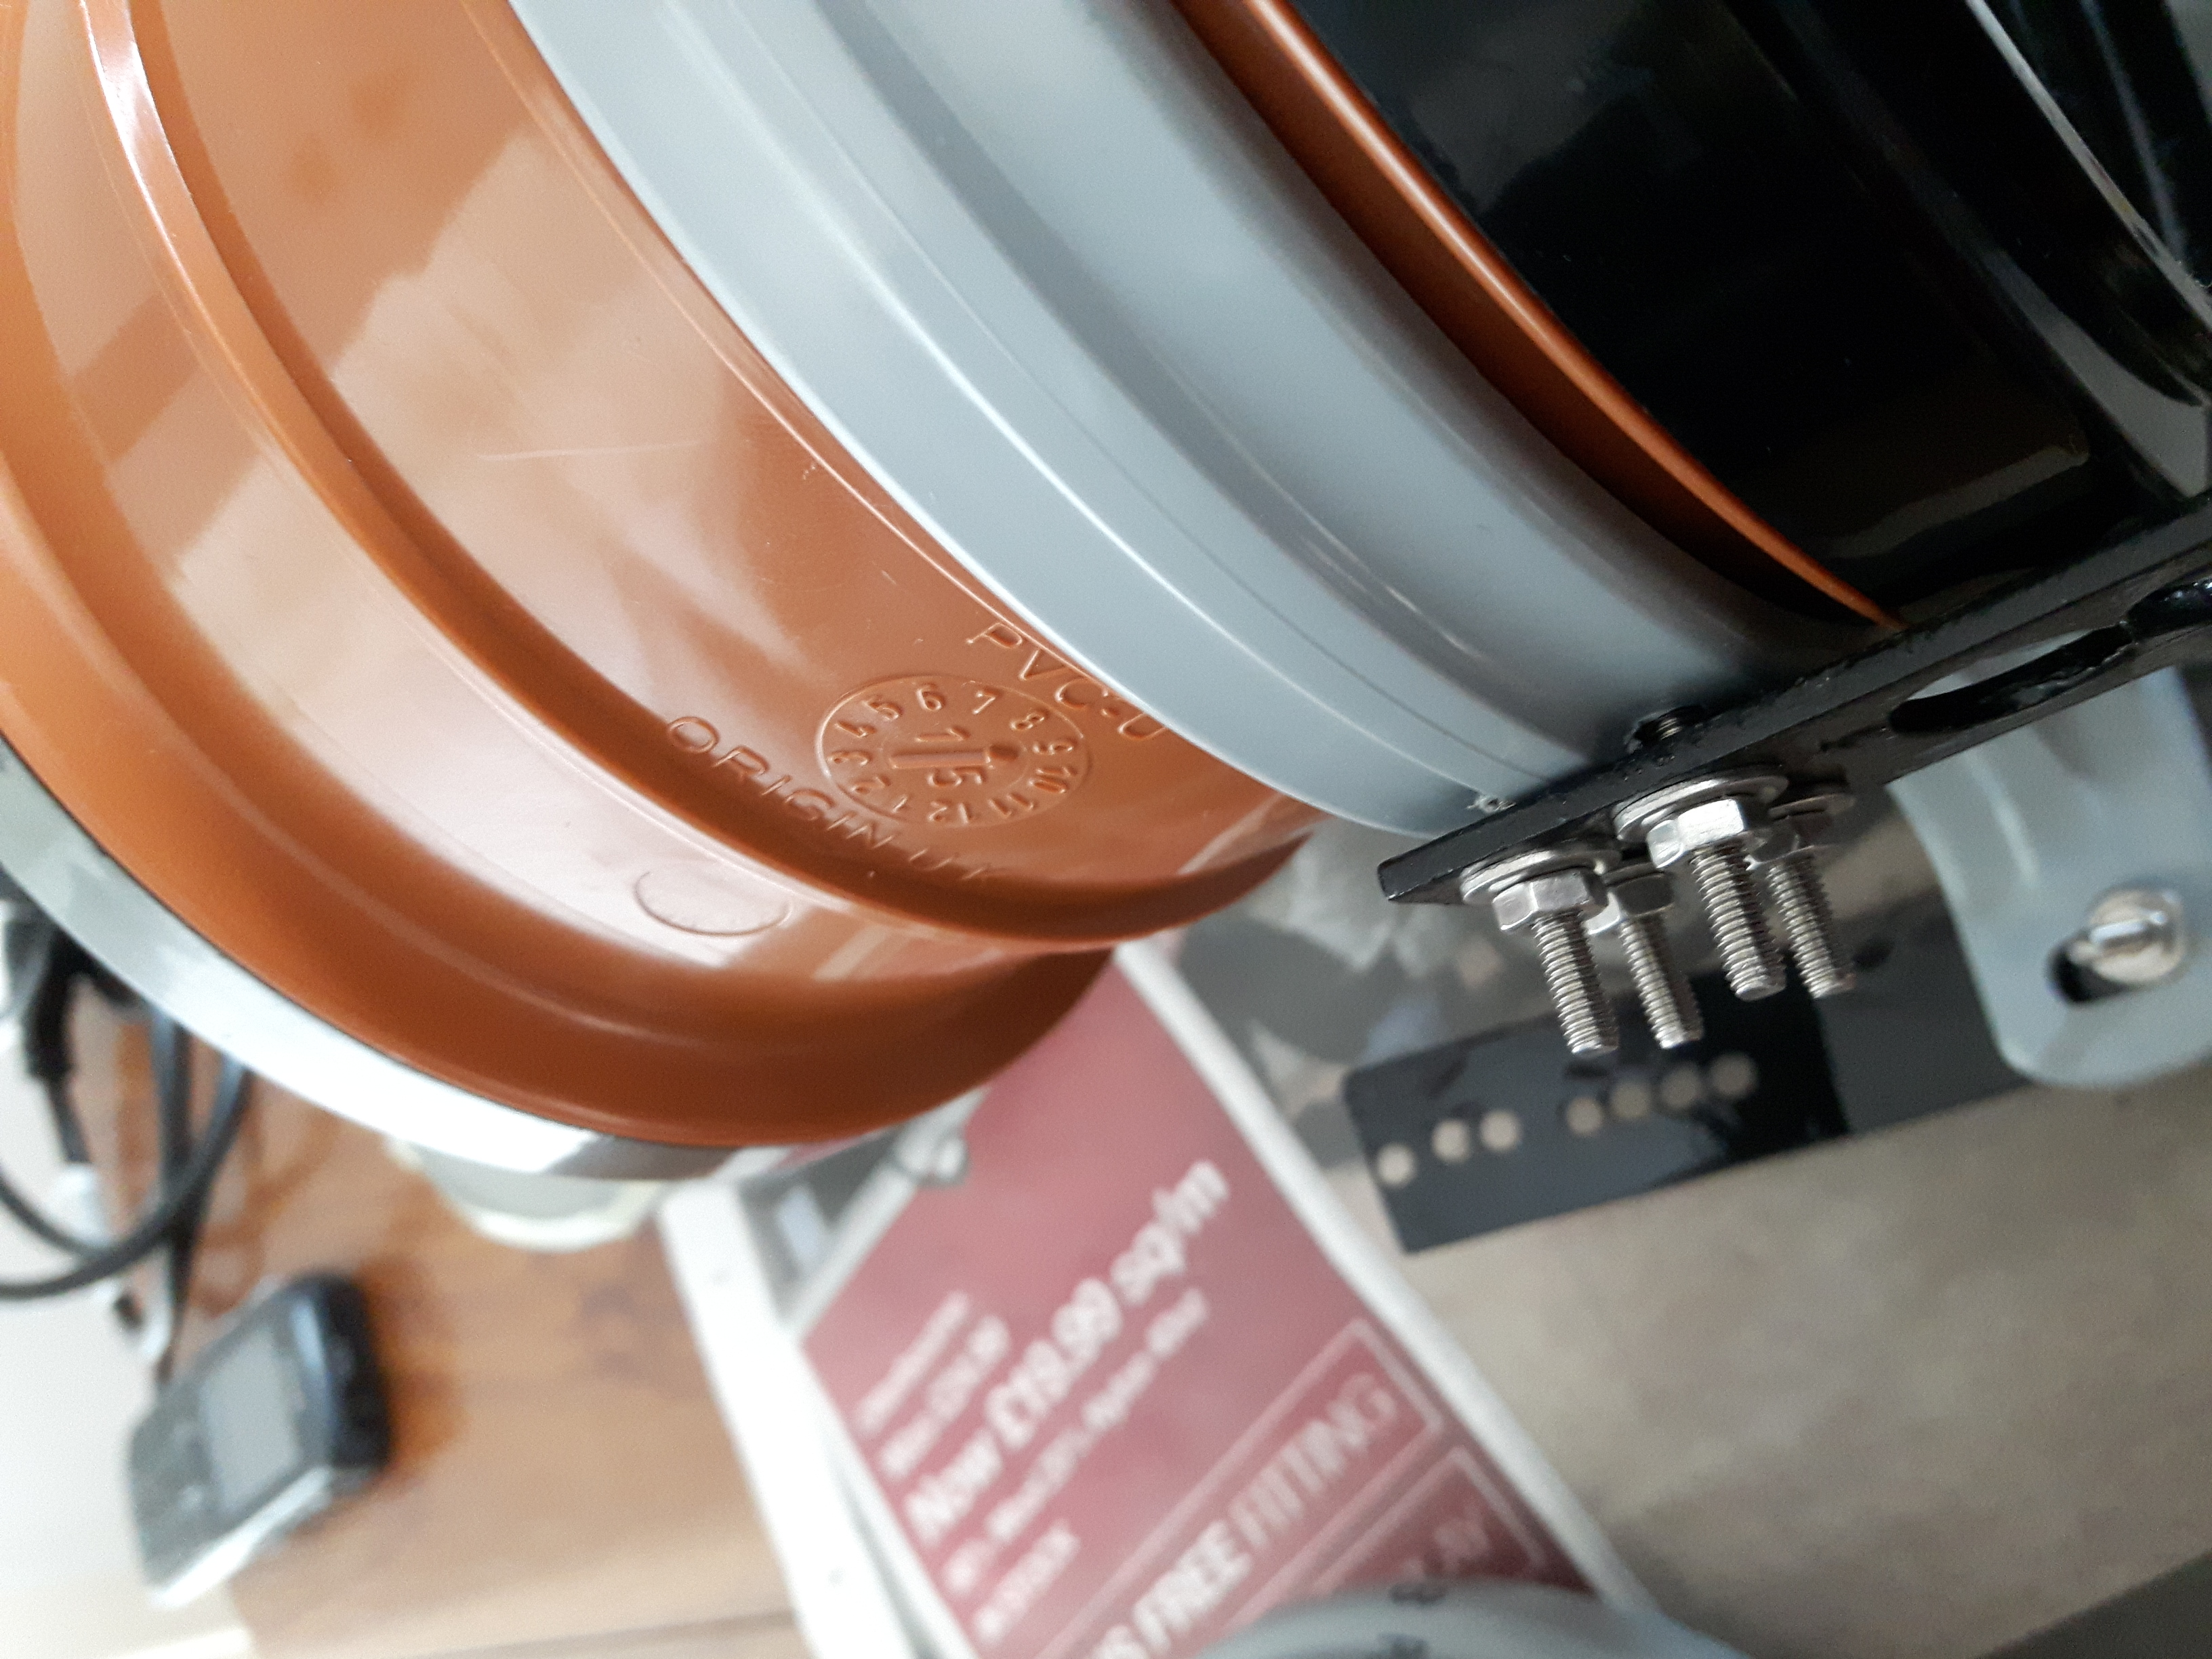
\includegraphics[width=\linewidth]{20160625_143939.jpg}
\end{minipage}
\caption{Using socket brackets to mount the steel structure onto the pressure vessel. One of the brackets is placed in the grooves in the double-socket pipe to stop them from slipping along the ROV.}
\label{fig:brackets}
\end{figure}

%-------------------------------------------------------------------------------
\subsection{Motor mounting}
Motors are bolted onto custom brackets made of bent steel (\unit[2 by 20]{mm} section) using M2.5 bolts. The motor manufacturer does not provide a~detailed drawing that specifies the location of the mounting holes. Therefore, the location of the holes was marked on the brackets by using the motors themselves as a~guide. To ensure that the motors rotate freely, they are separated from their brackets using two washers, as shown in Fig.~\ref{fig:motorMountingDetails:label:b}.

The vertical motor brackets are located in the approximate longitudinal centre of buoyancy (centre of the pressure vessel) to reduce the pitching moment that the vertical motors impart on the vehicle. Similarly, the horizontal motor brackets are mounted at the vertical centre of buoyancy. To reduce the number of the holes in the socket brackets, both sets of motor brackets are bolted onto the side longitudinals, which are then bolted onto the socket brackets, as shown in Fig.~\ref{fig:motorMountingDetails}.

\begin{figure}[htb]
\begin{center}
\begin{tabular}{c c}
	\subfloat[Back]
		{\includegraphics*[width=0.6\textwidth,angle=270]{20160625_143911.jpg}
		\label{fig:motorMountingDetails:label:a} } &
	\subfloat[Top]
		{\includegraphics*[width=0.6\textwidth,angle=270]{20160625_143928.jpg}
		\label{fig:motorMountingDetails:label:b} } \\
\end{tabular}
\end{center}
\caption{Details of mounting the motors onto the external steel structure. Views from the top and back of the vehicle.}
\label{fig:motorMountingDetails}
\end{figure}

%-------------------------------------------------------------------------------
\subsection{Ballast}
The ballast consists of two sets of elements: \unit[4 by 30]{mm} rolled steel flat-bar section cut to the length of the transverse clip stiffeners, and a~\unit[186]{mm} long, \unit[2 by 20]{mm} steel bar. The latter was a~left-over from the steel bought to manufacture the external frame.

Five of the \unit[4 by 30]{mm} sections are mounted close to the centre of gravity in order to compensate for the excess net buoyancy available from the hull. They are placed slightly forward to balance out the moment generated by the heavy wires and cables placed at the aft end. The smaller ballast bar is placed at the forward end of the sled and its exact position was adjusted to achieve an even trim. This was possible thanks to there being a~series of holes on either side of the sled, which allow fine-tuning of the ballast position. The arrangement of the ballast is indicated in Fig.~\ref{fig:rovGAsExternal}.

\clearpage % Avoid "too many unprocessed floats" error.

%===============================================================================
\section{Umbilical}\label{section:umbilical}

%-------------------------------------------------------------------------------
\subsection{Connector on the ROV}\label{ssection:connectorOnTheROV}
The connector enables the CAT5 cable and the shore power cable, which form the tether described in more detail in section~\ref{ssection:tether}, as well as the wires carrying signals from the ESCs to the motors described in section~\ref{ssection:propulsionSubsystem}, to penetrate inside the pressure vessel without compromising water tightness.

The connector is based on a~threaded PVC connector, the male part of which is shown in Fig.~\ref{fig:pvcConnector}. All the mentioned cables and wires were threaded through the male connector, which was then filled with a~two-part epoxy resin. All the wires were stripped out of their outermost covers as shown in Fig.~\ref{fig:strippingWires} to allow the resin to penetrate as deep into the wires as possible, to reduce the possibility of water dripping into the pressure vessel between the resin and the wires' cores. For the same reasons, the wires were separated from each other when applying the epoxy, as shown in Fig.~\ref{fig:separatingTheWires}. This ensured that some resin was present between all the wires.

Once complete, the male connector with wires laminated-in was screwed into the hole punched in the aft plug from its outer side, with PTFE tape used to seal the thread. Two rubber washers were placed on the connector, on both the inner and outer sides of the aft plug. A~complementary, female part of the PVC connector was then screwed onto the male counterpart to remove the voids between the washers and the PVC parts. Lastly, silicone was applied to the outer side of the aft plug to further seal the connector. The complete aft plug, with the connector screwed in and silicone applied, is shown in Fig.~\ref{fig:externalSideOfTheAftPlug}.

Banana connectors were soldered onto the motor wires. The motor wires were then connected to the motors, and the ESCs and the motor control board (described in section~\ref{ssection:propulsionSubsystem}) such that forward and upward thrust would be produced without the relays on the motor control board being activated. The wires were colour-coded to ease re-assembly in this configuration. Finally, after the final assembly, the wires were fixed using white electrical tape, which also isolates the banana connectors from each other. The colour coding of the motor wires and the white electrical tape can be seen in Fig.~\ref{fig:internalSideOfTheAftPlug}.

\begin{figure}[htb]
\begin{minipage}[b]{1\linewidth}
  \centering
	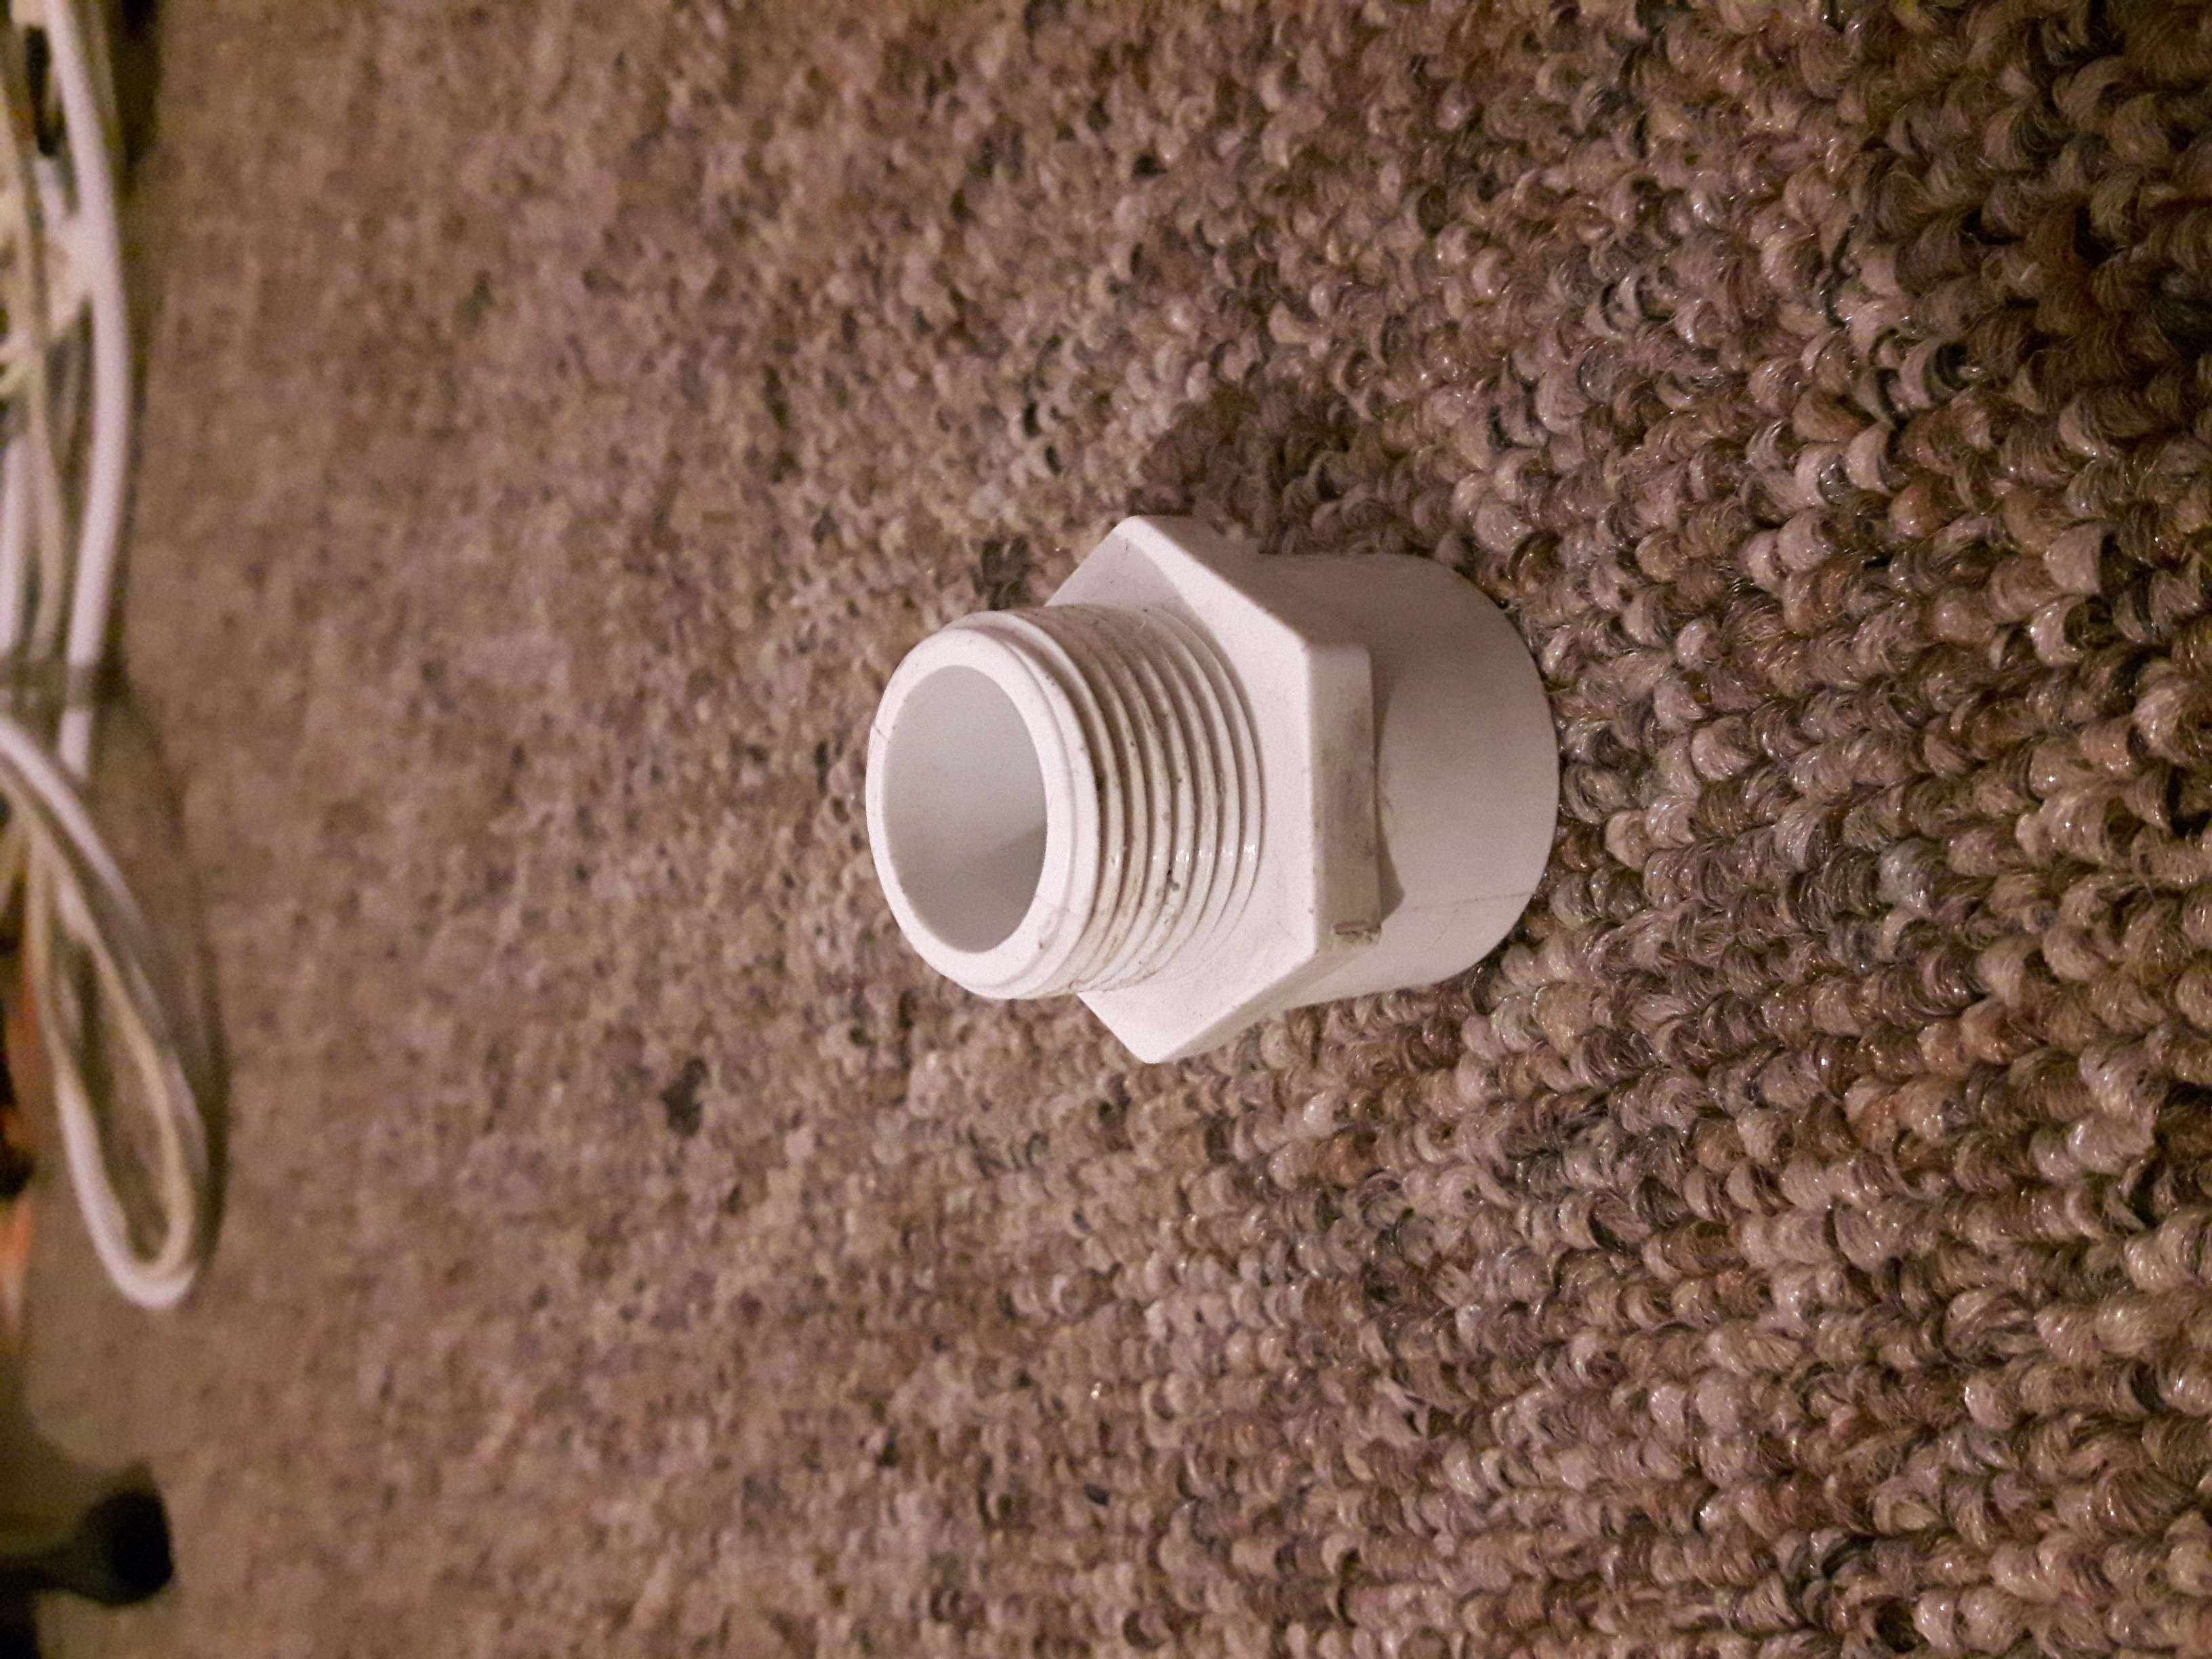
\includegraphics[width=\linewidth,angle=270]{20160826_213152.jpg}
\end{minipage}
\caption{Male part of the PVC connector through which the umbilical tether is threaded and then laminated.}
\label{fig:pvcConnector}
\end{figure}

\begin{figure}[htb]
\begin{center}
\begin{tabular}{c}
	\subfloat[Motor wires]
		{\includegraphics*[width=0.8\textwidth]{20160319_134634.jpg}
		\label{fig:strippingWires:label:a} } \\
	\subfloat[CAT5 cable]
		{\includegraphics*[width=0.8\textwidth]{20160319_131255.jpg}
		\label{fig:strippingWires:label:b} } \\
\end{tabular}
\end{center}
\caption{External cover of the wires is stripped so that less water drips through the umbilical connector once the wires are laminated in place.}
\label{fig:strippingWires}
\end{figure}

\begin{figure}[htb]
\begin{center}
\begin{tabular}{c c}
	\includegraphics*[width=0.6\textwidth,angle=270]{20160319_152814.jpg} & \includegraphics*[width=0.6\textwidth,angle=270]{20160319_153034.jpg} \\
\end{tabular}
\end{center}
\caption{Before laminating the wires into the PVC connector, they are separated to make sure some resin surrounds every wire and makes a~seal.}
\label{fig:separatingTheWires}
\end{figure}

\clearpage % Place these figures close to the text.

%-------------------------------------------------------------------------------
\subsection{Tether}\label{ssection:tether}
The umbilical tether consists of a~CAT5 cable, which extends the USB bus from the shore-based laptop to the ROV, as well as a~\unit[16]{A}-rated, three-chord power cable, which delivers battery power to the vehicle and grounds its structure. These two cables are held together by a~\unit[6]{mm} diameter nylon rope, which is tied around both cables at intervals of approximately one metre. The nylon rope can also be used to lift the vehicle or recover it from the water in case of failure. To this end, the nylon rope is mounted to the external steel structure of the ROV close to its centre of buoyancy. The steel structure provides a~strong mounting point, and the attachment location minimises the moments that the tether imparts on the vehicle, which makes it easier to operate. The location of the tether and the way it is attached to the ROV is shown in Fig.~\ref{fig:thetherOverview}.

During the initial towing tank test, described in section~\ref{section:manoeuvringTests}, it was discovered that the tether was too heavy and thus caused the ROV to sink, even though it was first made neutrally-buoyant on its own. To remedy this, bubble wrap was tied around the tether to increase its buoyancy. The bubble wrap was fixed with water-proof duct tape, as can be seen in Fig.~\ref{fig:thetherOverview}.

\begin{figure}[htb]
\begin{minipage}[b]{1\linewidth}
  \centering
	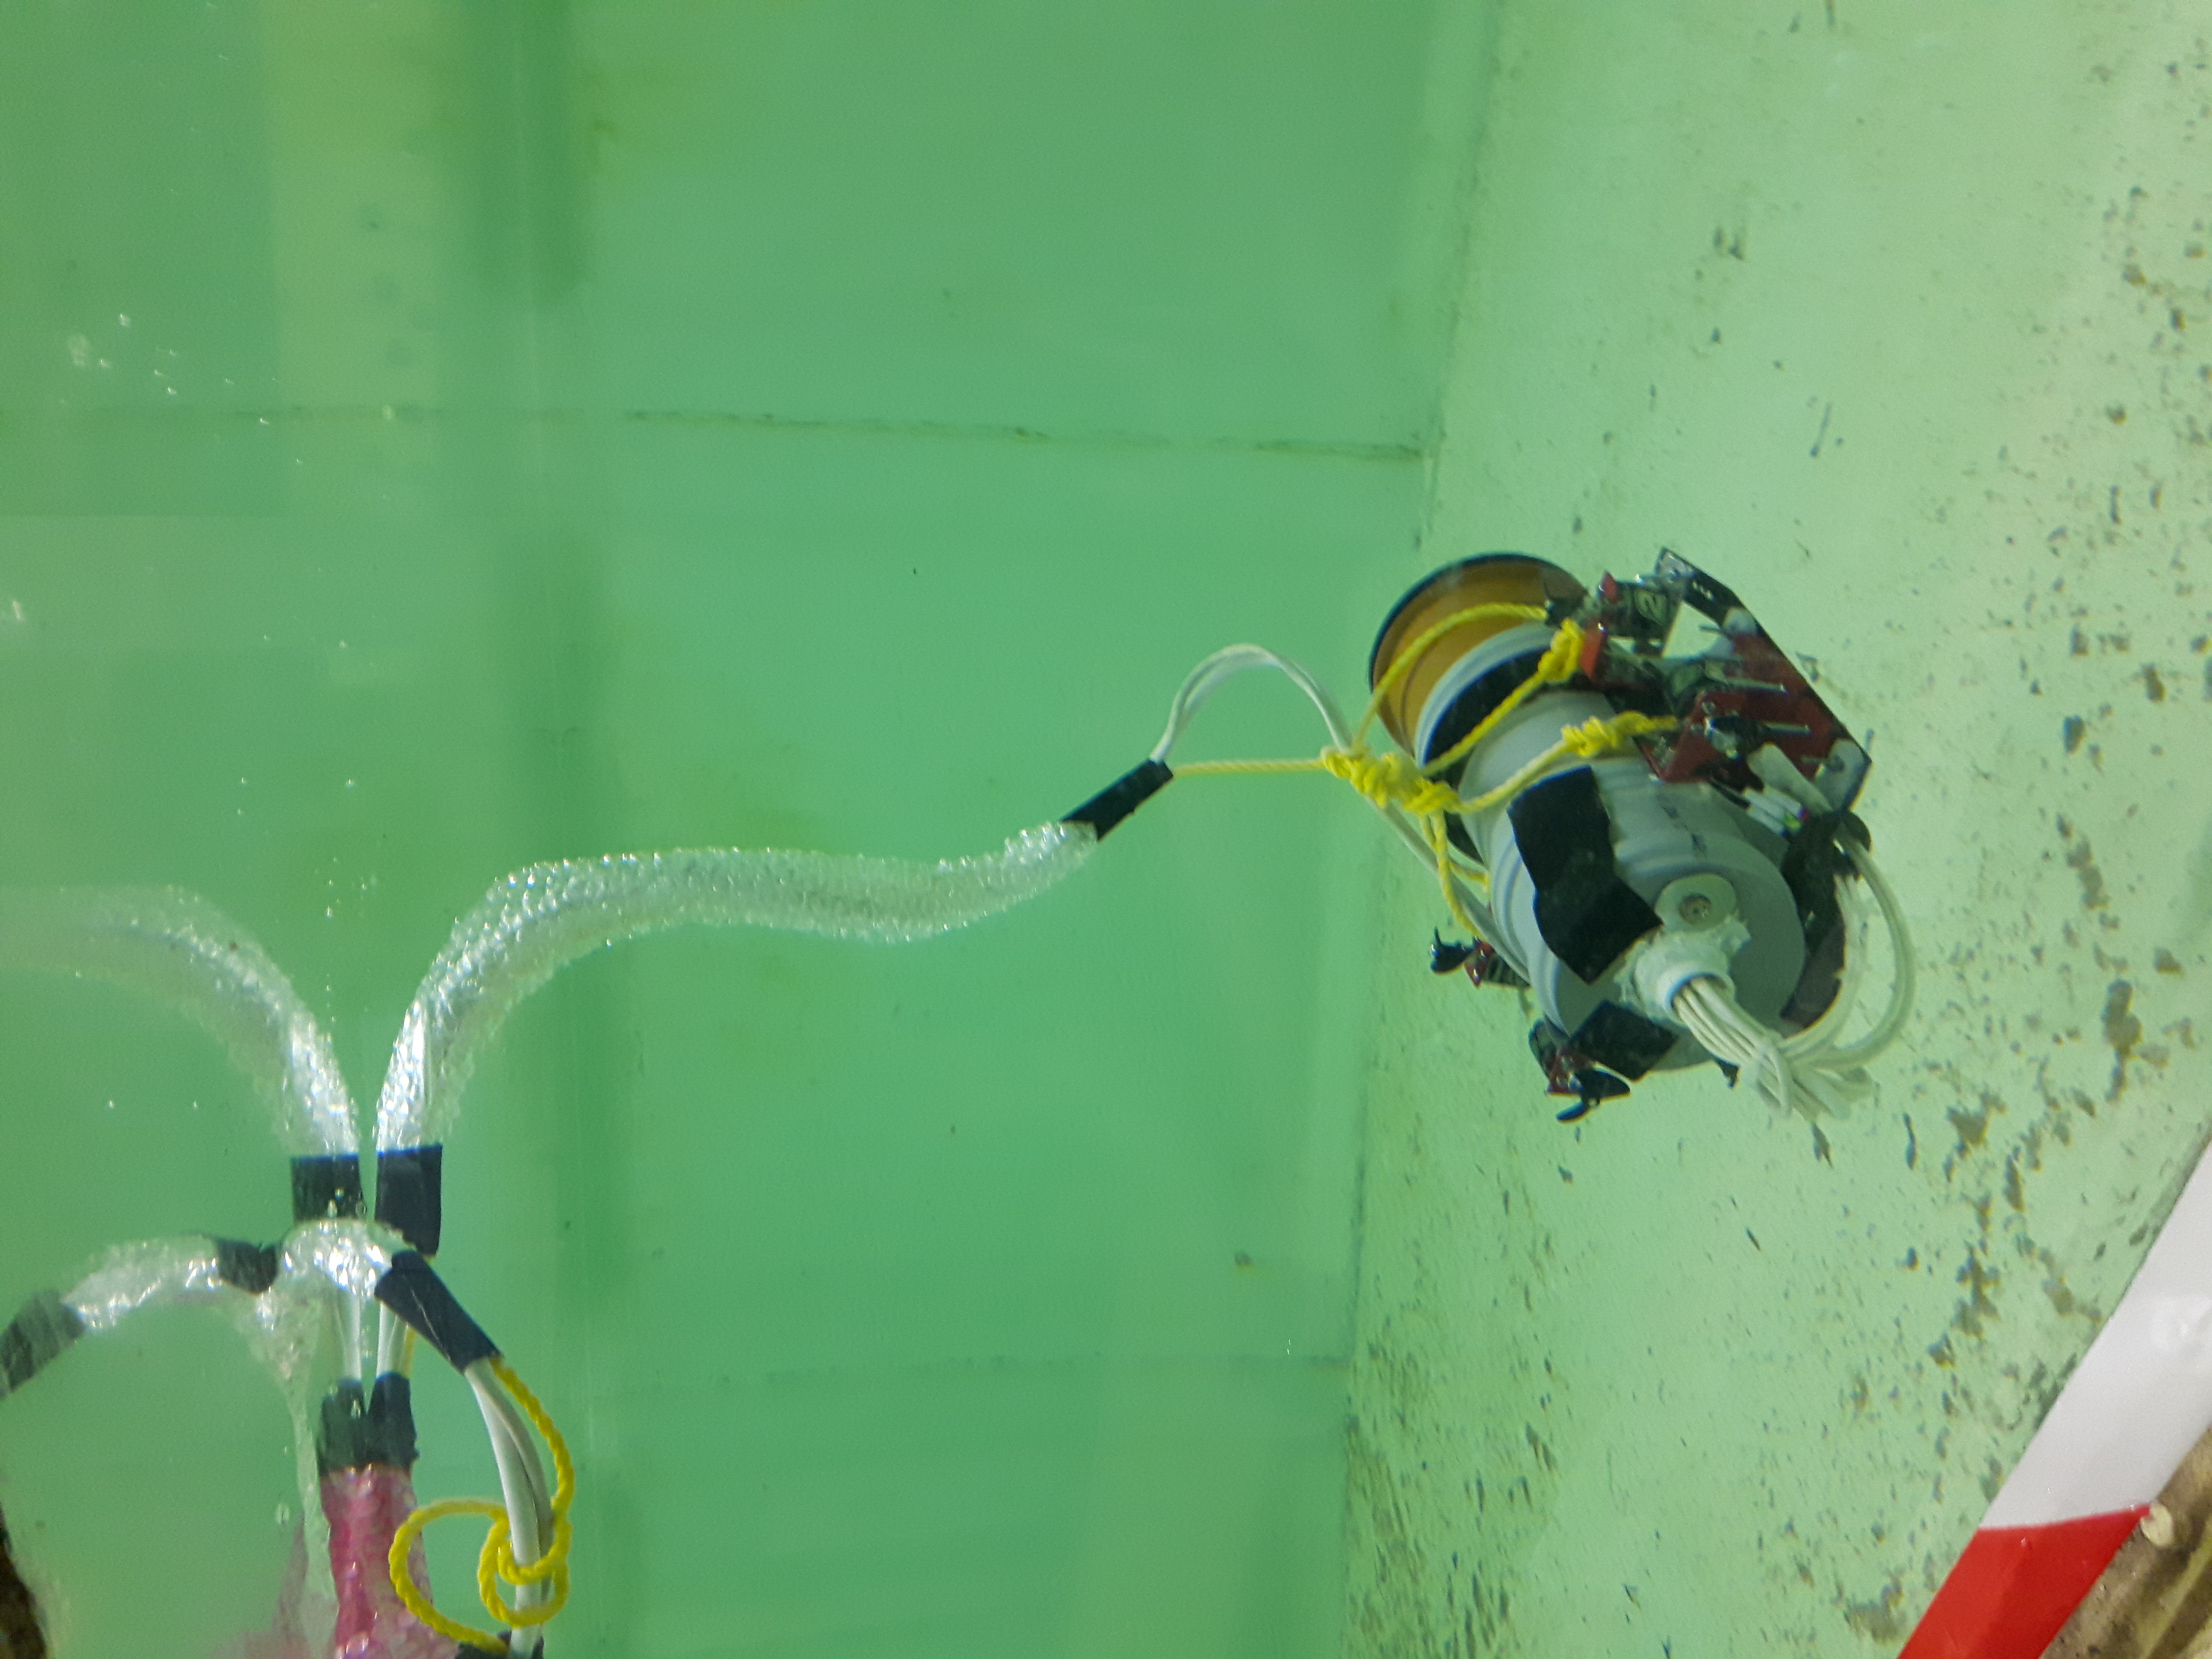
\includegraphics[width=\linewidth,angle=270]{20160826_135321.jpg}
\end{minipage}
\caption{Overview of the tether structure together with its attachment to the external steel structure.}
\label{fig:thetherOverview}
\end{figure}

\clearpage % Avoid "too many unprocessed floats" error.

\pagestyle{chapter-fancy-style}
\chapter{Software design}

%=====================
\section{Overview}
The ROV software can be split into two distinct parts - the code present on the Arduino, which translates the operator commands to physical actions of the vehicle, as well as the shore-based computer part, which collects the user inputs and sends the corresponding commands to the Arduino. The remainder of this chapter covers both parts of the software separately. The computer part of the code is intended as cross-platform because its based on Python~2.7 and its open-source libraries. However, it has been developed and tested exclusively on Ubuntu 12 and 14.

%=====================
\section{Micro-controller}

%---------------------
\subsection{Program structure}
The Arduino only receives and executes operator commands, which means its functional flow is rather simple, as shown in the flowchart in Fig.~\ref{fig:arduinoMainLoop}. The \texttt{execute every instruction in series block} might involve arming the ESCs, sending readings of all the sensors, switching the forward LEDs on or off, and setting thrust levels and directions of all the motors.

\begin{figure}[]
\centering
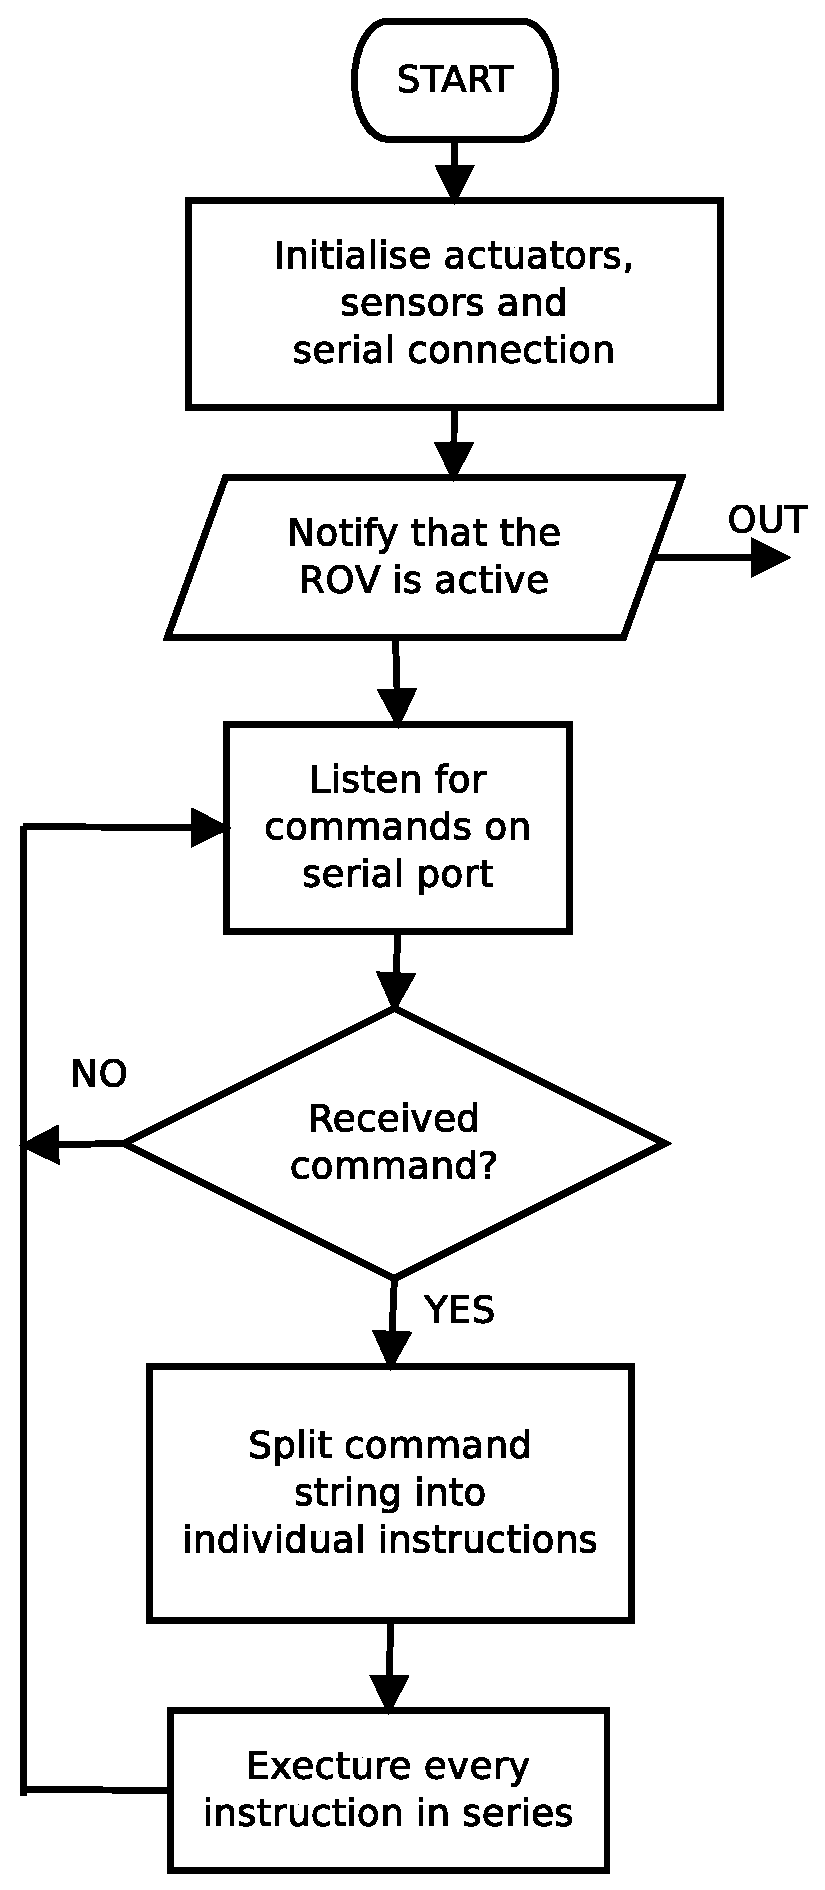
\includegraphics[width=0.4\linewidth]{arduinoSWFlowchart.eps}
\caption{Block diagram showing the flow of the Arduino \texttt{setup()} and \texttt{loop()} functions.}
\label{fig:arduinoMainLoop}
\end{figure}

%---------------------
\subsection{Hardware interfaces}
In order to interact with each piece of hardware, such as a sensor or electric motor, or in order to implement simple functionality, a special class \texttt{Module} has been implemented. This is holds fields such as \texttt{identifier} and \texttt{currentValue}, the combination of which is used to control a single aspect of the Arduino operation. For example, a~\texttt{Module} object called \texttt{refreshRate} holds the loop frequency the micro-controller operates at. Such basic objects typically get used directly in the \texttt{loop()} method and are treated as simple storage containers. For instance, at the end of each \texttt{loop()} call a new delay gets set as \texttt{delay(refreshRate.getValue());}, which allows setting the delay value using the same command protocol as used with more complex \texttt{Module}s.

Key methods of the \texttt{Module} class are the virtual \texttt{getValue()}, \texttt{setValue(int newValue)}, and \texttt{arm()} functions. Their default implementation in the \texttt{Module} class allows the user to read or set the value the object holds, for instance the refresh rate of the Arduino, or to initialise the object at the beginning of the execution.

Each of the modules gets created upon initialisation of the Arduino code and pointers to them are collected in arrays \texttt{Module* actuators[]} or \texttt{Module* sensors[]}, depending on their functionality. This arrangement allows the user to create classes derived from \texttt{Module} and overriding the functionality they execute when given or asked for a new value, at the same time allowing the same code in the main program loop to be used to interact with each object. A depiction of the currently used classes is shown in Figure \ref{fig:moduleClasses}. This approach is used primarily in the \texttt{parseInput()} method which is responsible for communication between the micro-controller and the PC or the \texttt{sendSensorReadings()} method which calls the \texttt{getValue()} function on each sensor module and encodes their readings into a string message which gets sent to the PC.

Currently implemented classes derived from \texttt{Module} are:
%
\begin{itemize}
\item \texttt{BrushlessDCMotor} - accepts negative and positive demand on the motor rps into the \texttt{setValue} function, treating negative values as reverse. Uses two assigned output pins in order to control the direction (binary digital output) and speed (PWM) of the motor via the ESC.
\item \texttt{LEDModule} - the value passed to the \texttt{setValue} method is treated as a binary switch telling the module to set the output pin either to HIGH or LOW state, thus controlling the LED.
\item \texttt{DepthSensor} - implements the \texttt{getValue()} method in order to return the current depth. Currently, this is a~\textbf{placeholder only}.
\end{itemize}

\begin{figure}[p]
\centering
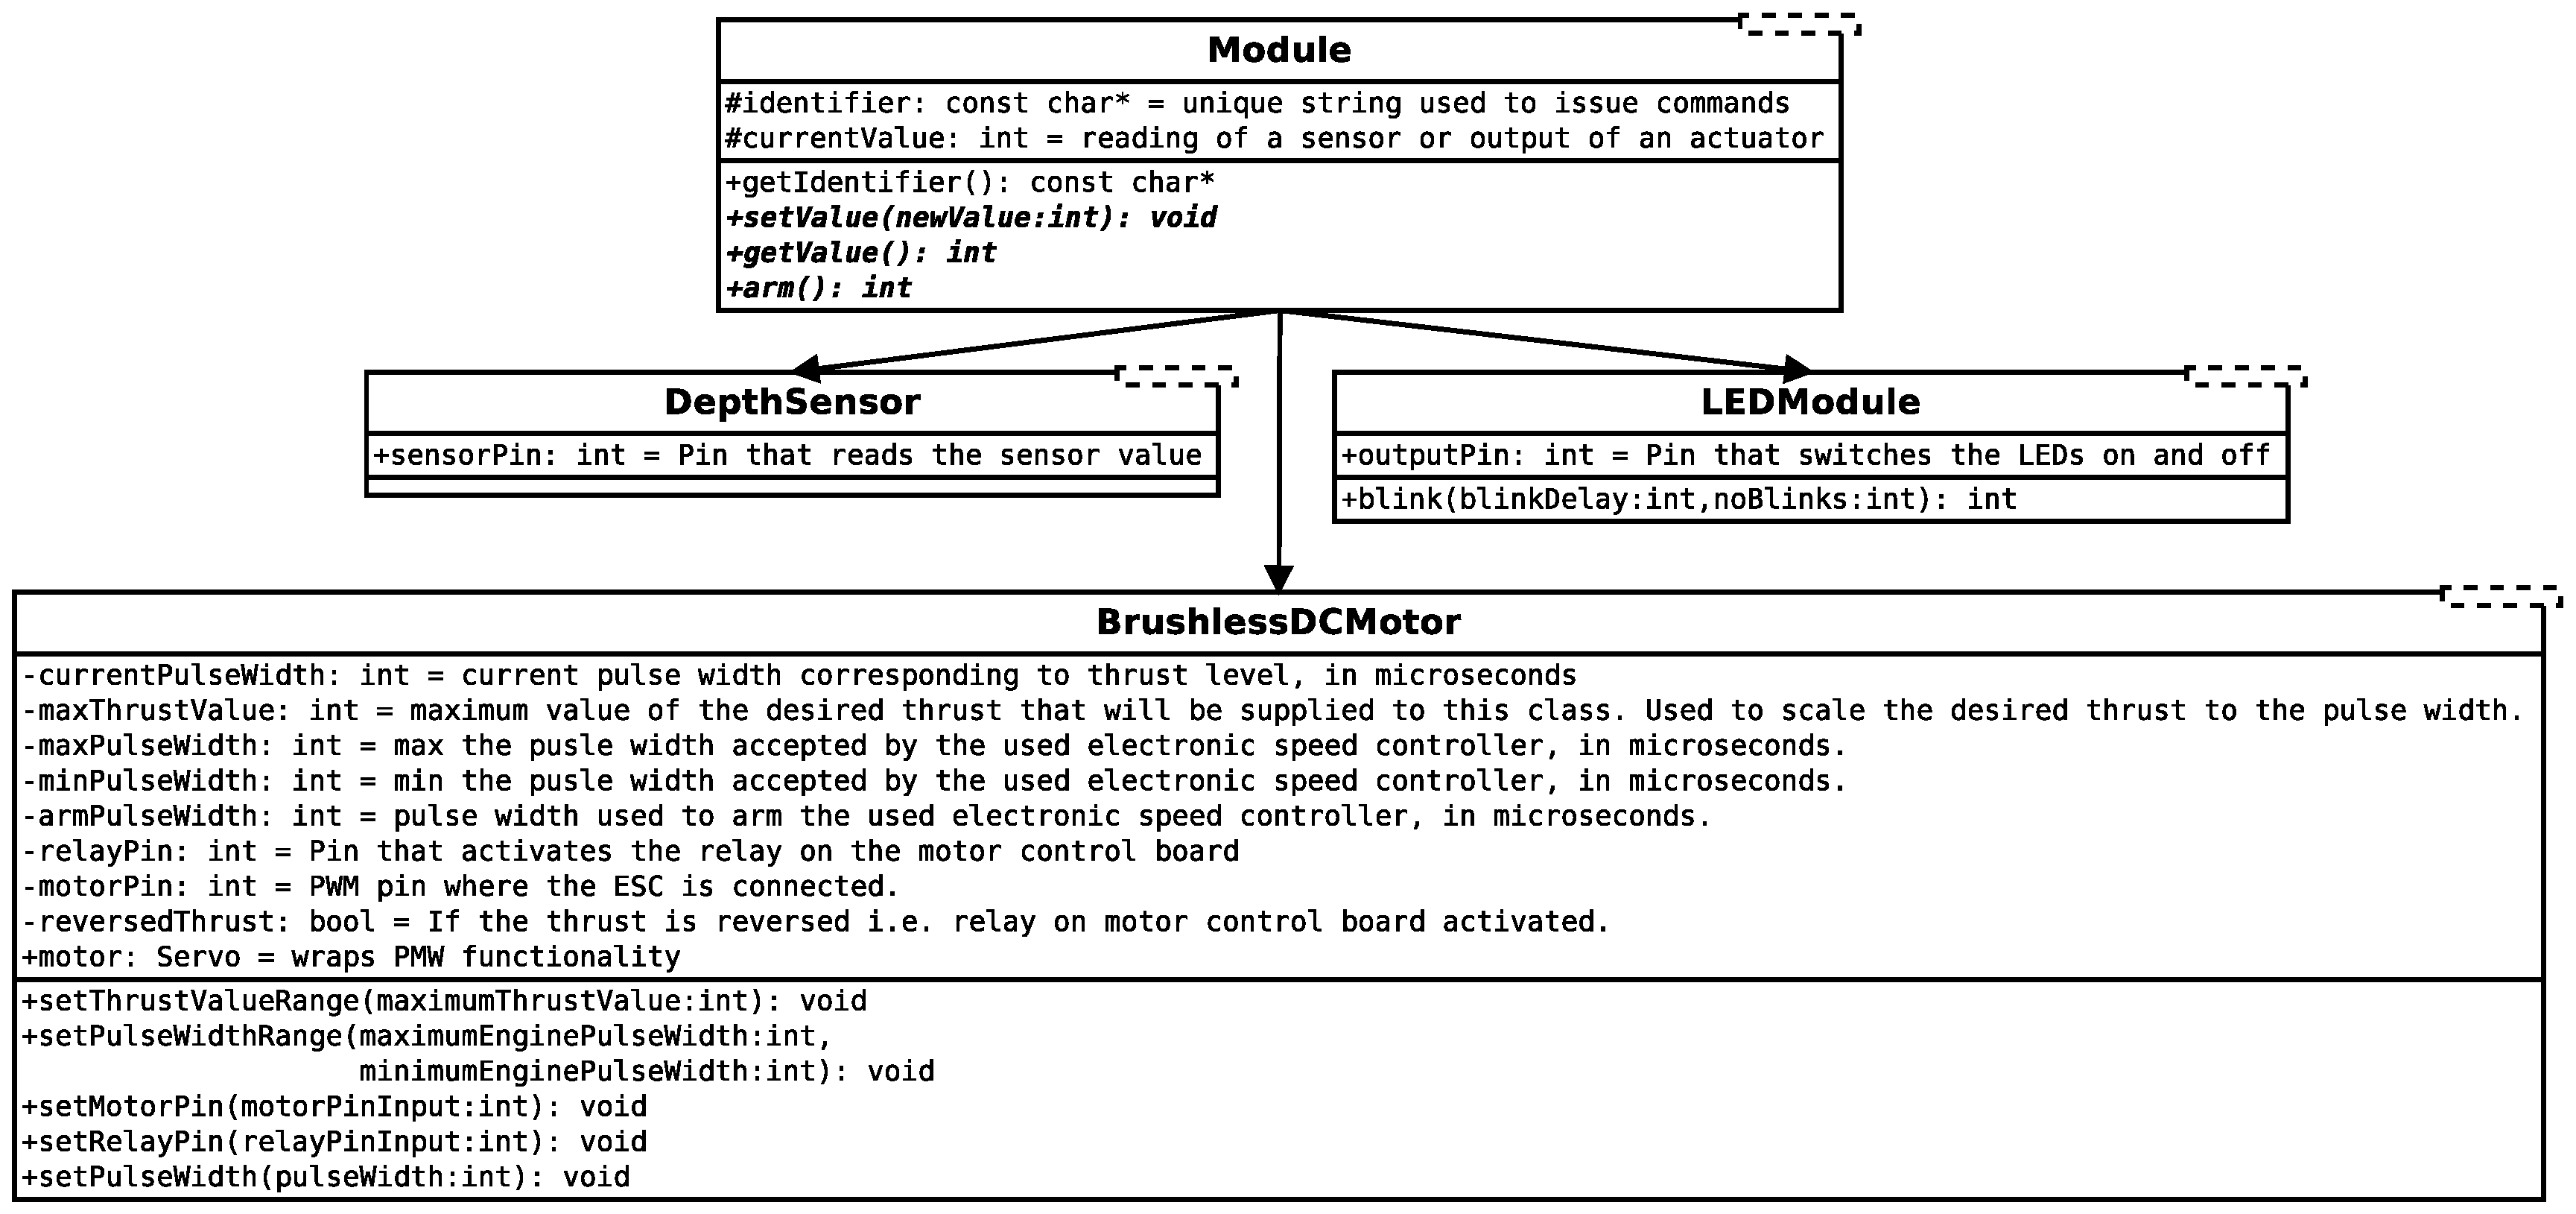
\includegraphics[width=0.8\textheight,angle=90]{ardunioSWClassDiagram.eps}
\caption{Block diagram showing the class hierarchy of the \texttt{Module} classes used to control Arduino functionality.}
\label{fig:moduleClasses}
\end{figure}

%---------------------
\subsection{Communications}

The ROV communicates with the computer via a serial port using the USB connection. The process involves encoding messages into one-line strings and dumping them into the buffer for the other side to see. This imposes a need for strict formatting of the message packets, which is described in Table \ref{tab:commsEncoding}. Each message consists of a string flag denoting an action or a subsystem, for instance "forwardLED" or "sendSensorReadings", followed by an integer value. An arbitrary number of commands may be sent in any one packet although the length of the entire message is limited by the character buffer size on the Arduino.

During each loop, the micro-controller attempts to read data from the serial port. If any data is found, the \texttt{parseInput()} method gets called. This is responsible for checking whether the passed information conforms to the message encoding system. If yes, the string gets unwrapped into a series of flags and corresponding values. Certain flags do not require the value and so an arbitrary integer may be passed, typically a 1 indicating a boolean true.

Each flag is then compared to the names of the registered \texttt{Module} objects until a match has been found. The value corresponding to the flag gets then passed using the virtual \texttt{setValue(int value)}. This is implemented by each class derived from the baseline \texttt{Module} class if a special action is required when a new value gets passed. For instance, the \texttt{BrushlessDCMotor} class converts the integer throttle demand into values understood by the ESC and adjusts the PWM signal, flipping the thrust direction relay if necessary. Other modules holding simple integer or boolean values do not re-implement the \texttt{setValue} method.

\begin{table}[h]
\centering
\caption{Description of the special characters used to format string messages sent over the serial port.}
\label{tab:commsEncoding}
\begin{tabular}{@{}ll@{}}
\toprule
\textbf{Character} & \textbf{Meaning} \\ \midrule
$<$ & beginning of message to PC \\
$>$ & beginning of message to Arduino \\
, & delimiter \\
; & end of message \\
\bottomrule
\end{tabular}
\end{table}

%=====================
\section{Computer}

%---------------------
\subsection{Program structure}
The key piece of code that runs as an executable is the \texttt{ROVgui.py}. It
defines a class \texttt{rovGuiMainFrame}, which then gets executed inside~a 
wxWidgets application. The class itself is derived from a~base class, which
defines the basic functionality of the graphical user interface alone (discussed
in more detail later) but all of the code responsible for the operation of the
ROV itself is contained in \texttt{ROVgui.py}.
The class contains several timers which execute specific methods at fixed intervals,
for instance they ask the mirco-controller to send the sensor readings or pass
demands for the electric motors.
Each of the key aspects of the code will be discussed in more detail in the following
parts of this chapter.

%---------------------
\subsection{Communications}
The protocol used to communicate with the micro-controller via the serial connection
utilises the \texttt{serial} Python library. This simply opens a port and treats
it as a buffer to read and write from. All of the parsed messages adhere to the
structure used by the Arduino side, namely begin and end with specific characters
and each element is separated by a known delimiter. The following code listing
provides a minimum example showing how a known port is opened, written into and
read from.

\begin{lstlisting}[style=myPythonStyle,language=Python]
import serial
import time

BAUD_RATE = 19200
REFRESH_RATE = 100
PORT = "/dev/ttyACM0"

# open the connection
serialConnection = serial.Serial(PORT, BAUD_RATE, timeout = 2)

testMsgGood = True
try:
    serialConnection.inWaiting()
except:
    testMsgGood = False

if not serialConnection or not serialConnection.readable() or not testMsgGood:
    raise IOError("Connection is FUBAR!")

# keep looping and printing whatever we get from the serial
message = ">sendSensorReadings,1;"
while True:
	serialConnection.write(message)
    line = serialConnection.readline().replace("\n","")
    if line:
        print line
    time.sleep(1./REFRESH_RATE)
\end{lstlisting}

%---------------------
\subsection{User input}
Interface to the Xbox controller (Figure \ref{fig:xboxController}) has been
created using pyGame 1.9.1, an open-source library for game development.
The interface relies on pyGame joystick module capturing all the inputs provided
by the user via the controller as events. These are stored in a buffer and then
the main GUI function periodically calls the \texttt{parseEvents()} method implemented
in the \texttt{controller} class. This retrieves the most recent set of events,
clears the buffer, and updates the values of axes and button positions held
inside the \texttt{controller} object. From here they are accessed from the main GUI each time a new
set of input parameters gets sent to the micro-controller.
A minimum working example which captures the events and prings the current axes
positions in the terminal is provided

\begin{lstlisting}[style=myPythonStyle,language=Python]
import pygame
from pygame.locals import *

pygame.init()
clock = pygame.time.Clock()

joysticks = []
for i in range(0, pygame.joystick.get_count()):
        joysticks.append(pygame.joystick.Joystick(i))
        joysticks[-1].init()
        print "Detected joystick '",joysticks[-1].get_name(),"'"
while 1:
        clock.tick(60)
        for event in pygame.event.get():
                if event.type == QUIT:
                        print "Received event 'Quit', exiting."
                        return
                elif event.type == KEYDOWN and event.key == K_ESCAPE:
                        print "Escape key pressed, exiting."
                        return
                elif event.type == KEYDOWN:
                        print "Keydown,",event.key
                elif event.type == KEYUP:
                        print "Keyup,",event.key
                elif event.type == MOUSEMOTION:
                        print "Mouse movement detected."
                elif event.type == MOUSEBUTTONDOWN:
                        print "Mouse button",event.button,"down at",pygame.mouse.get_pos()
                elif event.type == MOUSEBUTTONUP:
                        print "Mouse button",event.button,"up at",pygame.mouse.get_pos()
                        
                elif event.type == JOYAXISMOTION:
                        print "Joystick '",joysticks[event.joy].get_name(),"' axis",event.axis,"motion."
                        if event.axis == 2:
                                print ' axis 2', event.value
                        elif event.axis == 5:
                                print ' axis 5', event.value
                elif event.type == JOYBUTTONDOWN:
                        print ("Joystick '",joysticks[event.joy].get_name(),
                            "' button",event.button,"down.")
                elif event.type == JOYBUTTONUP:
                        print "Joystick '",joysticks[event.joy].get_name(),"' button",event.button,"up."
                elif event.type == JOYHATMOTION:
                        print "Joystick '",joysticks[event.joy].get_name(),"' hat",event.hat," moved to",event.value
\end{lstlisting}

\begin{figure}[]
\begin{center}
\includegraphics*[width=0.6\textwidth,angle=0]{xboxController.jpg}
\end{center}
\caption{USB Xbox controller used to provide control inputs to the ROV.}
\label{fig:xboxController}
\end{figure}

%---------------------
\subsection{Video acquisition}

In order to acquire imagery from the on-board USB camera, the code uses OpenCV 3.0.0-rc1,
a cross-platform, open-source digital imaging library. It is written in C++ but
provides a straightforward interface for use in Python.
In short, capturing a single frame is achieved as

\begin{lstlisting}[style=myPythonStyle,language=Python]
import cv2, wx
# create a camera
cameraID = 1
cameraCapture = cv2.VideoCapture(cameraID)
# get a picture and set up colours
ret, picture = cameraCapture.read()
height, width = picture.shape[:2]
picture = cv2.cvtColor(picture, cv2.COLOR_BGR2RGB)
# convert to wxWidgets bitmap for use inside the GUI
bmp = wx.BitmapFromBuffer(width, height, picture)
\end{lstlisting}

%---------------------
\subsection{Graphical interface}

Figure \ref{fig:GUI} shows the layout used to provide a graphical interface for
controlling the ROV. Live feed from the on-board camera is provided on the right-hand
side while the left is devoted to controlling the top-level functionality of the
vehicle. The top left-hand corner shows the thruster demand of each motor. Below,
controls are provided for the serial port connection to the Arduino, the video
feed of the camera, Xbox controller and arming of the electronic speed controllers
on board of the ROV.
There is also a pop-up Settings window which allows the user to adjust the
Arduino loop frequency, as well as frequencies for sending the control inputs,
receiving sensor readings, and camera frame rate.
The entire GUI runs on wxWidgets 2.8.12.1 and has been designed using wxFormBuilder,
both of which may be readily integrated with Python and are open-source.

\begin{figure}[]
\begin{center}
\includegraphics*[width=0.8\textwidth,angle=0]{GUI.png}
\end{center}
\caption{Graphical user interface (GUI) used to control the ROV from the laptop.}
\label{fig:GUI}
\end{figure}

\pagestyle{chapter-fancy-style}
\chapter{Testing}

%=====================
\section{Procedure}

The first stage of in-water tests was carried out in the Lamont
towing tank of the University of Southampton. Figure \ref{fig:testingSetup}
shows the experimental set-up used in the described tests.
The towing tank provided a~calm, controlled
environment without currents or wind. The water depth was under \unit[2]{metres},
which was deemed sufficient for the initial test of the pressure vessel.
Furthermore, the window in the side of the towing tank allowed easier observation
of the robot from the side.

There were three main tests to be carried out during the first series of testing:
\begin{enumerate}
\item  Testing of the power output of all the motors and making sure they can drive
	the vehicle in a steady and controlled manner. If not, adjusting the control
	inputs to compensate for any asymmetries
\item Verifying that the provided visual cues, proposed control interface, and
	available motor arrangements are suitable to allow a new user to operate the
	vehicle efficiently and perform simple tasks, such as inspection of underwater
	objects
\item Submerging the vehicle to progressively larger depths to test the water-
	tightness of the outer hull
\end{enumerate}

\begin{figure}[htb]
\begin{center}
\begin{tabular}{c c}
	\subfloat[Dry and manoeuvring tests]
		{\includegraphics*[width=0.45\textwidth,angle=270]{20160826_125304.jpg}
		\label{figure:testingSetup:label:a} } &
	\subfloat[For observation through side window]
		{\includegraphics*[width=0.45\textwidth,angle=270]{20160826_141659.jpg}
		\label{figure:testingSetup:label:b} } \\
\end{tabular}
\end{center}
\caption{View of the testing set-up in the Lamont towing tank.}
\label{fig:testingSetup}
\end{figure}

In order to comply with the health \& safety regulations, a strictly defined
procedure of using the ROV was put in placed and adhered to throughout the testing:
%
\begin{enumerate}
\item Plugging the ROV into a laptop via an Ethernet cable using a USB converter
\item Powering-up the motors using a 12 V DC power supply placed on-shore
\item Testing the camera system and ensuring each of the motors is operational
\item Placing the vehicle in the water using an insulated rod and an attachment point
	provided by the main tether
\item Performing the required tests and tasks
\item Surfacing the vehicle close to the operator and unplugging the power supply
\item Recovering the vehicle by hand and finishing the test
\end{enumerate}

%=====================
\section{Manoeuvring tests}\label{section:manoeuvringTests}

Before the towing tank tests it had been recognised that despite all electric
motors and electronic speed controllers being identical, the same demand signals
from the Arduino board made each of the motors rotate at a slightly different
speed. This had been identified by setting them to the highest RPM in pairs
and listening to the sound they produce while adjusting the tuning constants in order to eliminate the beat frequency (much like tuning a guitar). One of the
vertical thrusters proved to behave particularly differently than the others.
Its tuning parameters were thus adjusted in the Arduino script before the tests,
in order to achieve approximately identical RPM as the other vertical motor
with the same thrust demand.

Once the vehicle was placed in water its balance, initially tested in a small
water container, was verified. The predicted centre of gravity location agreed
well with the expectations, yielding neutral trim. At the outset of the tests
the vehicle was also neutrally buoyant and kept a steady altitude just below the
water surface. Placing the tether attachment at the centre of gravity negated
any moments and prevented the ROV from adopting excess trim angles.
At first, however, the tether was not as buoyant as initially hoped and was dragging
the robot down to the bottom. An impromptu solution was employed whereby sheets
of bubble wrap were attached at even intervals to the tether, making it neutrally
buoyant.

Then, several basic manoeuvres were attempted:
moving in a straight line horizontally and in the vertical plane, orienting the
ROV in a particular direction, and turning while under way.
It has been found that the used motors and propellers provide more than enough
thrust to make the vehicle agile and faster than expected. The control interface
also fulfilled its purpose well and allowed the operator to convey commands to
the ROV with ease. An example of a successful descent manoeuvre is seen in
Figure \ref{fig:rovThroughTheWindow}.
Due to the linear mapping of the joystick displacement to
thrust demand it was rather difficult for the operator to execute very precise
control over the vehicle, however. Such precise control requires very low levels
of thrust, which can only be obtained with minimal joystick displacements in the
current implementation.

It was also found that the tether, in particular the power cable, was so
stiff and twisted (it had spent most of its lifetime on a~reel prior to deployment)
that it made it difficult for the ROV to move freely. This is because the
twist in the tether exerted a~constant moment on the robot, which in turn
rotated the ROV around the tether. This meant that adopting
certain headings was impossible without constant actuation of the thrusters, for example.

It had also been expected that the load on the motors would increase significantly
when they operated in water instead of air, which was indeed observed. At first,
the battery system had been fitted with \unit[1]{A} fuse, which was sufficient
to operate four motors at their maximum thrusts in air. In water, however, 
the \unit[1]{A} fuse allowed the user to only operate the motors at very low RPMs
and made it difficult not to exceed the current limit, thus requiring a~fuse
replacement. In practice, only a~small deviation in the joystick position would
lead to burning the fuse. The internal electronics were capable of
sustaining higher currents and the \unit[1]{A} limit had been chosen somewhat
arbitrarily for increased safety. The safety concern was relaxed during the test
and a~\unit[4]{A} fitted instead. This allowed the user to operate the ROV 
without any restraint while still having a~safeguard built into the system.

\begin{figure}[htb]
\begin{center}
\includegraphics*[width=0.6\textwidth,angle=270]{20160826_135245.jpg}
\end{center}
\caption{ROV floating near the bottom of the towing tank.}
\label{fig:rovThroughTheWindow}
\end{figure}

%=====================
\section{Blind control tests}

Outside of control environment, the operator would not be able to see the ROV from their
workstation and instead they would have to rely solely on the visual and other
cues fed back to them from the on-board sensors. The next stage of tests focused
on simulating this scenario by placing the operator so that the ROV was outside
their field of view. They were then tasked with performing the same tasks as before
(simple manoeuvres - straight line, turning circle, ascent/descent, keeping
a constant heading) when relying only on the video feed from the USB camera
fitted to the ROV.

It has been found that latency present in the visual system was detrimental to
the user's ability to manoeuvre the vehicle easily. They were able to establish
the general direction the ROV was facing in relation to the main features of the
nearby environment. Doing so required them to put in considerable effort and
was further made difficult by the unpredictable forces and moments exerted by
the tether. The exact reason for the existence of latency in the video feed is
unclear - it could be due to the camera itself, due to the same CAT5 cable being
used to transfer video and serial commands to the Arduino, due to some issues
with the OpenCV library and its implementation in the current code, or due to
limitations of the current graphical user interface design.

Furthermore, it has been found that the 640x480 resolution of the camera is not
sufficient to provide detailed view of the ROV surroundings when the vehicle is
put in water with particulates in it. This made it difficult to judge the distance
of the vehicle from the obstacles ahead by using visual cues only.
Nonetheless, enough detail could be captured to allow key environmental
features to be distinguished, as seen in Fig.~\ref{fig:onBoardPictures}.

Lastly, the camera has a~considerable zoom. This makes approaching a~target at 
a~close distance dfficult because it seems to be much larger and thus closer than it in fact is.
At present, none of the ROV components are visible in the camera field of view.
Changing this, for example by using a~camera with a~wider field of view and moving
it further away from the pressure vessel surface, could help the operator judge
proximity to obstacles. This is because both the visible ROV components and the
obstacles would be distorted by the camera in the same way, and the relative
distance could be assessed.

\begin{figure}[htb]
\begin{center}
\begin{tabular}{c c}
	\subfloat[ROV on the free surface]
		{\includegraphics*[width=0.45\textwidth,angle=0]{20160826_135540162340_026.jpg}} &
	\subfloat[Wavemakers at the end of the tank]
		{\includegraphics*[width=0.45\textwidth,angle=0]{20160826_135540162340_539.jpg}} \\
	\subfloat[Operators seen through the side window of the tank]
		{\includegraphics*[width=0.45\textwidth,angle=0]{20160826_140221589085_280.jpg}} &
	\subfloat[The far end of the tank]
		{\includegraphics*[width=0.45\textwidth,angle=0]{20160826_150305045904_012.jpg}} \\
\end{tabular}
\end{center}
\caption{Video frames captured by the on-board camera during towing tank tests.}
\label{fig:onBoardPictures}
\end{figure}

%=====================
\section{Water-tightness tests}

Before the tests in the towing tank, the ROV had been submerged in a small water
container (i.e. a bath tub) for the period of several hours to verify the efficacy
of seals and connections. No water ingress had been observed even for overnight
immersion tests at the depth of approximately 30 cm.

The towing tank tests lasted approximately 3.5-4 hours, during which the ROV
was removed from the water several times. After the initial several seconds
after the first immersion no visible water bubbles were seen escaping from the
hull, indicating the hull remained watertight.
Throughout the tests, however, the vehicle was observed to gradually lose its
neutral buoyancy. Towards the end of the trials, the ROV would linger close to the
tank bottom, and making it ascend using the thrusters alone became difficult.
After the final test run, the aft plug was removed and a~small amount of water was
seen to leak from inside the pressure vessel. The exact volume was not verified due to lack of
experience of the operators. It was sufficient to adversely affect the neutral buoyancy
of the vehicle but did not reach the electronics, which suggests the leak was
small. It is believed the water ingress took place through the aft seal between
the hull and removable aft plug as it was at this location that small air bubbles
were seen escaping at the beginning of each series of tests.
The aft cable port could also be the culprit, although this is seen as less likely.





%%% Conclusions
\pagestyle{chapter-fancy-style}
\chapter{Conclusions}

%=====================
\section{Summary of the design}

It has been demonstrated that even within a~limited budged of less than £300 and
access only to basic tools, a~fully-functional remotely operated underwater vehicle 
can be designed, manufactured and tested.
The overall design concept using only four degrees of freedom control and employing
a compact vehicle shape has proven to provide sufficient performance that would be
expected of a low-cost sensor platform for use in shallow waters.
Several specific aspects of the design should be refined but a precious
few have also proven to be quite successful. Each of these groups will be discussed
in more detail in the subsequent parts of this chapter.

%=====================
\section{Successful design features}

Several of the chosen engineering solutions have been found to work particularly
well during the tests. These were:
%
\begin{itemize}
\item Using the on-board Arduino micro-controller to allow control of the ROV
	from a standard laptop has proven to be a very flexible and low-cost solution
\item The X-Box controller used to collect input data has been found to provide
	a robust, easy-to-use interface
\item Overall general arrangement of the vehicle has been successful and integrating
	all of the electronics into a removable internal frame allowed ease of access
	during assembly and disassembly
\item Placing the motors so that their thrust passes through the centre of gravity
	has allowed problem-free operation in the 4 DoF framework
\item Use of an external power source allowed the vehicle to be compact and
	lightweight, with the complete system fitting into an above-average sized
	rucksack and being easily transportable by hand.
\end{itemize}

%=====================
\section{Recommendations for future designs}

Despite the general success of the project, several aspects of the design could,
and a few certainly should, be improved if a next iteration or a brand new vehicle
were to be designed. These summarise the lessons learned through the development
and testing of the ROV:
%
\begin{itemize}
\item Making the aft plug removable without the use of bolts or other permanent
	connectors made it very easy to assemble the vehicle on-shore but led to
	the vehicle not being completely watertight. This is a major issue which
	could be addressed by i) using a threaded aft plug with a better seal
	ii) use of a slot-in plug secured with nuts and fitted with additional o-rings
	iii) manufacturing the pressure hull from a less compressible material (steel
	or aluminium) and desigining bespoke watertight connections
\item Removing pre-twist from the tether and making it float would make manoeuvring
	the vehicle far easier
\item Fixing the video latency issue would be necessary for operation in a real
	environment. This may require using a dedicated VGA cable, a different camera,
	or better implementation of the current software
\item At present the motors are placed in water without waterproofing which would not
	be acceptable in the long term in real environments such as seas or rivers.
	A watertight enclosure would be necessary, most likely utilising a magnetic
	coupling, to prevent corrosion of the motors.
\item Being able to redirect a time trace of control inputs and sensor readings to a file
	would make analysing the performance of the vehicle easier
\item In the present design only the internal structure was grounded, extending this
	to include all steel elements would add an important safety feature
\item Using non-linear mapping or having two sensitivity settings for the controller
	should make it easier to perform precise manoeuvres
\item Adding a sensor measuring power output of the battery would be an important
	indicator of the efficiency of the vehicle and would allow planning missions more accurately
\item At present, each of the power wires in the connector in the aft plug (section~\ref{ssection:connectorOnTheROV})
	ends with a~banana connector. Grouping the cables by the corresponding motors
	and using a~single connector for each motor
	would streamline the ROV assembly process significantly.
\item At present, the external steel frame is difficult to disassemble or even
	detach from the central hull due to the way the bolts are situated. At the
	time it was not considered crucial to allow this but having such a possibility
	would allow modifications to the design to be introduced more easily.
\item The electrical system has been significantly over-designed in most places
	in terms of current ratings. However, there are several segments with much lower
	safety factors, which effectively dictate the maximum safe power output from the battery.
	A~careful choice of suitable current ratings for each segment of the design would allow a~much
	more efficient overall system design.
\item Currently used off-the-shelf electronic speed controllers are straightforward
	to utilise but require a~large amount of wiring to operate, which takes up a~considerable
	amount of internal volume of the ROV. Using PCB-mounted variants or even controlling
	the motors directly from the Arduino by pulsing current using transistors could
	allow for a much more compact design. Ultimately, a~small PCB for a~single motor
	or a~pair of motors could be devised. The PCBs could be connected using stack-through
	connectors, thus eliminating most of the wiring used in the current design. This
	would make the system more modular, and lower-mass and thus also smaller and more agile.
\item Having the tether attach to the inspection hatch (aft plug) poses certain difficulties
	during disassembly as often multiple connectors have to be disconnected and reconnected
	just to allow a simple task to be accomplished. Moving the cable port to a stationary part
	of the hull could simplify these operations.
\item Adding controller calibration constants to the GUI settings window would make it more
	easily adjustable by the user.
\end{itemize}


%\bibliography{../library}{}
%\bibliographystyle{ieeetr}

%%% Appendix
\begin{appendix}

\end{appendix}

\end{document}

